%  A simple AAU report template.
%  2015-05-08 v. 1.2.0
%  Copyright 2010-2015 by Jesper Kjær Nielsen <jkn@es.aau.dk>
%
%  This is free software: you can redistribute it and/or modify
%  it under the terms of the GNU General Public License as published by
%  the Free Software Foundation, either version 3 of the License, or
%  (at your option) any later version.
%
%  This is distributed in the hope that it will be useful,
%  but WITHOUT ANY WARRANTY; without even the implied warranty of
%  MERCHANTABILITY or FITNESS FOR A PARTICULAR PURPOSE.  See the
%  GNU General Public License for more details.
%
%  You can find the GNU General Public License at <http://www.gnu.org/licenses/>.
%
%  A simple AAU report template.
%  2015-05-08 v. 1.2.0
%  Copyright 2010-2015 by Jesper Kjær Nielsen <jkn@es.aau.dk>
%
%  This is free software: you can redistribute it and/or modify
%  it under the terms of the GNU General Public License as published by
%  the Free Software Foundation, either version 3 of the License, or
%  (at your option) any later version.
%
%  This is distributed in the hope that it will be useful,
%  but WITHOUT ANY WARRANTY; without even the implied warranty of
%  MERCHANTABILITY or FITNESS FOR A PARTICULAR PURPOSE.  See the
%  GNU General Public License for more details.
%
%  You can find the GNU General Public License at <http://www.gnu.org/licenses/>.
%
\documentclass[11pt,twoside,a4paper,openright]{report}
%%%%%%%%%%%%%%%%%%%%%%%%%%%%%%%%%%%%%%%%%%%%%%%%
% Language, Encoding and Fonts
% http://en.wikibooks.org/wiki/LaTeX/Internationalization
%%%%%%%%%%%%%%%%%%%%%%%%%%%%%%%%%%%%%%%%%%%%%%%%
% Select encoding of your inputs. Depends on
% your operating system and its default input
% encoding. Typically, you should use
%   Linux  : utf8 (most modern Linux distributions)
%            latin1
%   Windows: ansinew
%            latin1 (works in most cases)
%   Mac    : applemac
% Notice that you can manually change the input
% encoding of your files by selecting "save as"
% an select the desired input encoding.
\usepackage[utf8]{inputenc}
% Make latex understand and use the typographic
% rules of the language used in the document.
\usepackage{subfig}
\usepackage{capt-of}
\usepackage[danish,english]{babel}
% Use the palatino font
\usepackage[sc]{mathpazo}
\linespread{1.05}         % Palatino needs more leading (space between lines)
% Choose the font encoding
\usepackage[T1]{fontenc}
%%%%%%%%%%%%%%%%%%%%%%%%%%%%%%%%%%%%%%%%%%%%%%%%
% Graphics and Tables
% http://en.wikibooks.org/wiki/LaTeX/Importing_Graphics
% http://en.wikibooks.org/wiki/LaTeX/Tables
% http://en.wikibooks.org/wiki/LaTeX/Colors
%%%%%%%%%%%%%%%%%%%%%%%%%%%%%%%%%%%%%%%%%%%%%%%%
% load a colour package
\usepackage{xcolor}
\definecolor{aaublue}{RGB}{33,26,82}% dark blue
% The standard graphics inclusion package
\usepackage{graphicx}
% Set up how figure and table captions are displayed
\usepackage{caption}
\captionsetup{%
  font=footnotesize,% set font size to footnotesize
  labelfont=bf % bold label (e.g., Figure 3.2) font
}
% Make the standard latex tables look so much better
\usepackage{array,booktabs}
\usepackage{tabularx}
% Enable the use of frames around, e.g., theorems
% The framed package is used in the example environment
\usepackage{framed}

%%%%%%%%%%%%%%%%%%%%%%%%%%%%%%%%%%%%%%%%%%%%%%%%
% Mathematics
% http://en.wikibooks.org/wiki/LaTeX/Mathematics
%%%%%%%%%%%%%%%%%%%%%%%%%%%%%%%%%%%%%%%%%%%%%%%%
% Defines new environments such as equation,
% align and split
\usepackage{amsmath}
% Adds new math symbols
\usepackage{amssymb}
% Use theorems in your document
% The ntheorem package is also used for the example environment
% When using thmmarks, amsmath must be an option as well. Otherwise \eqref doesn't work anymore.
\usepackage[framed,amsmath,thmmarks]{ntheorem}

%%%%%%%%%%%%%%%%%%%%%%%%%%%%%%%%%%%%%%%%%%%%%%%%
% Page Layout
% http://en.wikibooks.org/wiki/LaTeX/Page_Layout
%%%%%%%%%%%%%%%%%%%%%%%%%%%%%%%%%%%%%%%%%%%%%%%%
% Change margins, papersize, etc of the document
\usepackage[
  inner=28mm,% left margin on an odd page
  outer=41mm,% right margin on an odd page
  ]{geometry}
% Modify how \chapter, \section, etc. look
% The titlesec package is very configureable
\usepackage{titlesec}
\titleformat{\chapter}[display]{\normalfont\huge\bfseries}{\chaptertitlename\ \thechapter}{20pt}{\Huge}
\titleformat*{\section}{\normalfont\Large\bfseries}
\titleformat*{\subsection}{\normalfont\large\bfseries}
\titleformat*{\subsubsection}{\normalfont\normalsize\bfseries}
%\titleformat*{\paragraph}{\normalfont\normalsize\bfseries}
%\titleformat*{\subparagraph}{\normalfont\normalsize\bfseries}

% Clear empty pages between chapters
\let\origdoublepage\cleardoublepage
\newcommand{\clearemptydoublepage}{%
  \clearpage
  {\pagestyle{empty}\origdoublepage}%
}
\let\cleardoublepage\clearemptydoublepage

% Change the headers and footers
\usepackage{fancyhdr}
\pagestyle{fancy}
\fancyhf{} %delete everything
\renewcommand{\headrulewidth}{0pt} %remove the horizontal line in the header
\fancyhead[RE]{\small\nouppercase\leftmark} %even page - chapter title
\fancyhead[LO]{\small\nouppercase\rightmark} %uneven page - section title
\fancyhead[LE,RO]{\thepage} %page number on all pages
% Do not stretch the content of a page. Instead,
% insert white space at the bottom of the page
\raggedbottom
% Enable arithmetics with length. Useful when
% typesetting the layout.
\usepackage{calc}

%%%%%%%%%%%%%%%%%%%%%%%%%%%%%%%%%%%%%%%%%%%%%%%%
% Bibliography
% http://en.wikibooks.org/wiki/LaTeX/Bibliography_Management
%%%%%%%%%%%%%%%%%%%%%%%%%%%%%%%%%%%%%%%%%%%%%%%%
\usepackage[backend=bibtex,
  bibencoding=utf8,sorting=none
  ]{biblatex}
\addbibresource{bib/mybib}

\usepackage{csquotes}

%%%%%%%%%%%%%%%%%%%%%%%%%%%%%%%%%%%%%%%%%%%%%%%%
% Our own stuff
%%%%%%%%%%%%%%%%%%%%%%%%%%%%%%%%%%%%%%%%%%%%%%%%
%needed for one table
\usepackage{multirow}
%needed for a different table
\newcolumntype{Y}{>{\centering\arraybackslash}X}

%needed for code listings
\usepackage{listings}
%sets the language globally to C
\lstset{language=C}
%code formating
\usepackage{adjustbox}
\usepackage{float}
%\usepackage[usenames,dvipsnames]{xcolor}

\definecolor{codegreen}{rgb}{0,0.6,0}
\definecolor{codegray}{rgb}{0.5,0.5,0.5}
\definecolor{codepurple}{rgb}{0.58,0,0.82}
\definecolor{backcolour}{rgb}{0.95,0.95,0.92}
\definecolor{keywordblue}{rgb}{0.1,0,1}

\lstdefinestyle{CStyle}{
    backgroundcolor=\color{backcolour},
    commentstyle=\color{codegreen},
    keywordstyle=\color{keywordblue},
    numberstyle=\tiny\color{codegray},
    stringstyle=\color{codepurple},
    basicstyle={\footnotesize\ttfamily},
    breakatwhitespace=true,
    breaklines=true,
    captionpos=t,
    keepspaces=true,
    numbers=left,
    numbersep=5pt,
    showspaces=false,
    showstringspaces=false,
    showtabs=false,
    tabsize=2,
    language=C
}
\lstset{style=CStyle}

%%%%%%%%%%%%%%%%%%%%%%%%%%%%%%%%%%%%%%%%%%%%%%%%
% Misc
%%%%%%%%%%%%%%%%%%%%%%%%%%%%%%%%%%%%%%%%%%%%%%%%
% Add bibliography and index to the table of
% contents
\usepackage[nottoc]{tocbibind}
% Add the command \pageref{LastPage} which refers to the
% page number of the last page
\usepackage{lastpage}
% Add todo notes in the margin of the document
\usepackage[
%  disable, %turn off todonotes
  colorinlistoftodos, %enable a coloured square in the list of todos
  textwidth=\marginparwidth, %set the width of the todonotes
  textsize=scriptsize, %size of the text in the todonotes
  ]{todonotes}

%%%%%%%%%%%%%%%%%%%%%%%%%%%%%%%%%%%%%%%%%%%%%%%%
% Hyperlinks
% http://en.wikibooks.org/wiki/LaTeX/Hyperlinks
%%%%%%%%%%%%%%%%%%%%%%%%%%%%%%%%%%%%%%%%%%%%%%%%
% Enable hyperlinks and insert info into the pdf
% file. Hypperref should be loaded as one of the
% last packages
\usepackage{hyperref}
\hypersetup{%
	%pdfpagelabels=true,%
	plainpages=false,%
	pdfauthor={Bucur, Busemann, Klein},%
	pdftitle={P3 project},%
	pdfsubject={Pathfinding, as used in Rescuing Robots},%
	bookmarksnumbered=true,%
	hidelinks,		%no boxes aroundlinks and black fontcolor
	colorlinks=false,%
	citecolor=black,%
	filecolor=black,%
	linkcolor=black,% you should probably change this to black before printing
	urlcolor=black,%
	pdfstartview=FitH%
}
%%%%%%%%%%%%%%%%%%%%%%%%%%%%%%%%%%%%%%%%%%%%%%%%%%%%%%%%%%%%%%%%%%%%%%%%%%%%%%%%%%%%%%%%%%%%%%%%
%%%%%%%%%%%%%%%%%	OUR STUFF
\usepackage{nicefrac}
\newcommand*\mean[1]{\overline{#1}}

%%COLORS FOR COLORCODING FILES IN TODOS%%
\definecolor{c00}	{RGB}{200,200,082}%Acronyms \& Nomenclature
\definecolor{c01}	{RGB}{000,200,082}%Introduction
\definecolor{c02}	{RGB}{200,082,000}%Problem Description
\definecolor{c03}	{RGB}{082,100,200}%Problem Definition
\definecolor{c04}	{RGB}{100,050,200}%Development
  \definecolor{c04a}{RGB}{255,020,200} %Conventional Boost Converter
  \definecolor{c04b}{RGB}{010,200,200} %Switched Inductor
  \definecolor{c04c}{RGB}{200,200,200} %Single Switch Quadratic BC
  \definecolor{c04d}{RGB}{200,200,000} %Three Level BC
  \definecolor{c04x}{RGB}{004,229,069} %Cockroft Walton
  \definecolor{c04y}{RGB}{169,220,090} %Multilevel BC
\definecolor{c05}	{RGB}{050,100,150}%Implementation
  \definecolor{c05a}{RGB}{255,220,000} %Component Specifications
  \definecolor{c05b}{RGB}{210,000,200} %Driver
  \definecolor{c05c}{RGB}{200,200,200} %PCB Design
  \definecolor{c05d}{RGB}{000,200,200} %
  \definecolor{c05x}{RGB}{004,029,249} %
  \definecolor{c04y}{RGB}{069,120,250} %
\definecolor{c06}	{RGB}{150,100,150}%Testing
\definecolor{c07}	{RGB}{050,100,050}%Discussion
\definecolor{c08}	{RGB}{150,100,000}%Conclusion
\definecolor{c09}	{RGB}{050,200,050}%Perspective
\usepackage{pdfpages}
% package inclusion and set up of the document
% see, e.g., http://en.wikibooks.org/wiki/LaTeX/Formatting#Hyphenation
% for more information on word hyphenation
\hyphenation{ex-am-ple hy-phen-a-tion short}
\hyphenation{long la-tex}%
%  A simple AAU report template.
%  2015-05-08 v. 1.2.0
%  Copyright 2010-2015 by Jesper Kjær Nielsen <jkn@es.aau.dk>
%
%  This is free software: you can redistribute it and/or modify
%  it under the terms of the GNU General Public License as published by
%  the Free Software Foundation, either version 3 of the License, or
%  (at your option) any later version.
%
%  This is distributed in the hope that it will be useful,
%  but WITHOUT ANY WARRANTY; without even the implied warranty of
%  MERCHANTABILITY or FITNESS FOR A PARTICULAR PURPOSE.  See the
%  GNU General Public License for more details.
%
%  You can find the GNU General Public License at <http://www.gnu.org/licenses/>.
%
%
%
% see, e.g., http://en.wikibooks.org/wiki/LaTeX/Customizing_LaTeX#New_commands
% for more information on how to create macros

%%%%%%%%%%%%%%%%%%%%%%%%%%%%%%%%%%%%%%%%%%%%%%%%
% Macros for the titlepage
%%%%%%%%%%%%%%%%%%%%%%%%%%%%%%%%%%%%%%%%%%%%%%%%
%Creates the aau titlepage
\newcommand{\aautitlepage}[3]{%
  {
    %set up various length
    \ifx\titlepageleftcolumnwidth\undefined
      \newlength{\titlepageleftcolumnwidth}
      \newlength{\titlepagerightcolumnwidth}
    \fi
    \setlength{\titlepageleftcolumnwidth}{0.5\textwidth-\tabcolsep}
    \setlength{\titlepagerightcolumnwidth}{\textwidth-2\tabcolsep-\titlepageleftcolumnwidth}
    %create title page
    \thispagestyle{empty}
    \noindent%
    \begin{tabular}{@{}ll@{}}
      \parbox{\titlepageleftcolumnwidth}{
        \iflanguage{danish}{%
          
\includegraphics[width=\titlepageleftcolumnwidth]{figures/aau_logo_da}
        }{%
          
\includegraphics[width=\titlepageleftcolumnwidth]{figures/aau_logo_en}
        }
      } &
      \parbox{\titlepagerightcolumnwidth}{\raggedleft\sf\small
        #2
      }\bigskip\\
       #1 &
      \parbox[t]{\titlepagerightcolumnwidth}{%
      \textbf{Abstract:}\bigskip\par
        \fbox{\parbox{\titlepagerightcolumnwidth-2\fboxsep-2\fboxrule}{%
          #3
        }}
      }\\
    \end{tabular}
    \vfill
    \iflanguage{danish}{%
      \noindent{\footnotesize\emph{Rapportens indhold er frit tilgængeligt, men offentliggørelse (med kildeangivelse) må kun ske efter aftale med forfatterne.}}
    }{%
      \noindent{\footnotesize\emph{The content of this report is freely available, but publication (with reference) may only be pursued due to agreement with the authors.}}
    }
    \clearpage
  }
}

%Create english project info
\newcommand{\englishprojectinfo}[8]{%
  \parbox[t]{\titlepageleftcolumnwidth}{
    \textbf{Title:}\\ #1\bigskip\par
    \textbf{Theme:}\\ #2\bigskip\par
    \textbf{Project Period:}\\ #3\bigskip\par
    \textbf{Project Group:}\\ #4\bigskip\par
    \textbf{Participant(s):}\\ #5\bigskip\par
    \textbf{Supervisor(s):}\\ #6\bigskip\par
    \textbf{Copies:} #7\bigskip\par
    \textbf{Page Numbers:} \pageref{LastPage}\bigskip\par
    \textbf{Date of Completion:}\\ #8
  }
}

%Create danish project info
\newcommand{\danishprojectinfo}[8]{%
  \parbox[t]{\titlepageleftcolumnwidth}{
    \textbf{Titel:}\\ #1\bigskip\par
    \textbf{Tema:}\\ #2\bigskip\par
    \textbf{Projektperiode:}\\ #3\bigskip\par
    \textbf{Projektgruppe:}\\ #4\bigskip\par
    \textbf{Deltager(e):}\\ #5\bigskip\par
    \textbf{Vejleder(e):}\\ #6\bigskip\par
    \textbf{Oplagstal:} #7\bigskip\par
    \textbf{Sidetal:} \pageref{LastPage}\bigskip\par
    \textbf{Afleveringsdato:}\\ #8
  }
}

%%%%%%%%%%%%%%%%%%%%%%%%%%%%%%%%%%%%%%%%%%%%%%%%
% An example environment
%%%%%%%%%%%%%%%%%%%%%%%%%%%%%%%%%%%%%%%%%%%%%%%%
\theoremheaderfont{\normalfont\bfseries}
\theorembodyfont{\normalfont}
\theoremstyle{break}
\def\theoremframecommand{{\color{gray!50}\vrule width 5pt \hspace{5pt}}}
\newshadedtheorem{exa}{Example}[chapter]
\newenvironment{example}[1]{%
		\begin{exa}[#1]
}{%
		\end{exa}
}% my new macros

\begin{document}
%frontmatter
\pagestyle{empty} %disable headers and footers
\pagenumbering{roman} %use roman page numbering in the frontmatter
\newcommand{\HRule}{\rule{\linewidth}{0.5 mm}}
\begin{titlepage}

\begin{center}
% Upper part of the page
\iflanguage{danish}{%
	
\includegraphics[width=0.6\textwidth]{figures/aau_logo_da}
}{%
	
\includegraphics[width=0.6\textwidth]{figures/aau_logo_en}
}\\[0.5cm]

\textsc{\Large P5}\\[0.6cm]

% Title
\HRule \\[0.8cm]
{ \Huge \bfseries  Cool Title}\\[0.4cm]

  \Large{ - and subtitulatsia -
  % insert your subtitle here
  }
\HRule \\[1.2cm]

% Author and supervisor
\begin{minipage}{0.49\textwidth}
\begin{flushleft} \large
\emph{Students:}\\
Daniel Frederik Busemann\\
Ilian Oleg Haralampiev\\
Ivan Petrov Kulin\\
Simon Thies\\
\end{flushleft}
\end{minipage}
\begin{minipage}{0.49\textwidth}
\begin{flushright} \large
\emph{Supervisors:} \\
Sanjeevikumar Padmanaban
\end{flushright}
\end{minipage}

\vfill

% Bottom of the page
{\large \today}



\end{center}

\end{titlepage}

\thispagestyle{empty}
{\small
\strut\vfill % push the content to the bottom of the page
\noindent Copyright \copyright{} Aalborg University 2018\par
\vspace{0.2cm}
\noindent \LaTeX \: was used for typesetting this report,
MatLab, Simulink, EAGLE and LTSpice were used for designing and verifying the converter and
GitHub \cite{GitHub} for collaborating as a group.
}
\clearpage
\pdfbookmark[0]{Abstract and Information}{label:titlepage_en}
\aautitlepage{%
  \englishprojectinfo{
    %title 
    Non-inverting Multilevel\\
    DC-DC Boost Converter For\\
    Photovoltaic Applications
  }{%
    Signal Processing%theme
  }{%
    Fall Semester 2018 %project period
  }{%
    ED5-3-F18 % project group %TODO
  }{%
    %list of group members
    Daniel Frederik Busemann\\
    Ilian Oleg Haralampiev\\
    Ivan Petrov Kulin\\
    Simon Thies
  }{%
    %ls
    Sanjeevikumar Padmanaban
  }{%
    1 % number of printed copies
  }{%
    \today % date of completion
  }%
}{%department and address
  \textbf{Electronics and Computer Engineering}\\
  Aalborg University\\
  \href{http://www.aau.dk}{http://www.aau.dk}
}{% the abstract
	This report focuses on developing and testing a suitable DC-DC converter for PV applications.
	
	The main goal is to analyse, simulate and compare different topologies and choose the most efficient one. The chosen topology has been tested in hardware as well, to determine its real world viability and how accurate simulations are compared to real measurements.
	The topology chosen is far superior to the the conventional boost converter, as it has gain 6 times higher on all duty cycles. 
	
	For simulation the tools used are SIMULINK and LTSpice. For the hardware test a custom PCB has been designed and printed with a SKYPER driver board being used to operate the circuit.
	
}
\cleardoublepage
\cleardoublepage
\chapter*{Preface\markboth{Preface}{Preface}}\label{ch:preface}
\addcontentsline{toc}{chapter}{Preface}
This report was made by three students from Aalborg University Esbjerg attending
the 4th semester of the Electronics and Computer Engineering course.
From this point on,
every mention of \textbf{we}, \textbf{the group} or \textbf{the authors} refers to the three co-authors listed below.

All resources produced for this project can be found on the GitHub repository \cite{GitHub}.
Selected resources are also in the appendix.

\vspace{\baselineskip}\hfill Aalborg University, \today
\vfill\noindent

\begin{center}
\begin{minipage}[b]{0.45\textwidth}
 \centering
 \rule{\textwidth}{0.5pt}\\
  Daniel Frederik Busemann\\
 {\footnotesize <dbusem16@student.aau.dk>}
\end{minipage}
\hfill
\begin{minipage}[b]{0.45\textwidth}
 \vspace{20mm}
 \centering
 \rule{\textwidth}{0.5pt}
    Ilian Oleg Haralampiev\\
 {\footnotesize <iharal16@student.aau.dk>}
\end{minipage}
\hfill
%
\begin{minipage}[b]{0.45\textwidth}
 \vspace{20mm}
 \centering
 \rule{\textwidth}{0.5pt}\\
    Ivan Petrov Kulin\\
 {\footnotesize <ikulin16@student.aau.dk>}
\end{minipage}
\hfill
\begin{minipage}[b]{0.45\textwidth}
 \vspace{20mm}
 \centering
 \rule{\textwidth}{0.5pt}
    Simon Thies\\
 {\footnotesize <sthies16@student.aau.dk>}
\end{minipage}
\hfill
\end{center}

%
\includepdf[pages=-]{sections/preface.pdf} %TODO this is where the signed page goes
\pdfbookmark[0]{Contents}{label:contents}
\pagestyle{fancy} %enable headers and footers again
\tableofcontents
\listoffigures
\listoftodos
\cleardoublepage
%mainmatter
\pagenumbering{arabic} %use arabic page numbering in the mainmatter
\vspace{-24mm}
\section*{Acronyms \& Nomenclature}

\begin{tabular*}{\textwidth}{@{\extracolsep{\fill}} l l r}
	\textbf{Symbol}	& \textbf{Definition}			& \textbf{Unit}\\
	\hline
	AC			& Alternating Current				& \\
	BC			& Boost Converter					& \\
	C			& Capacitance						& $F$\\
	CBC			& Conventional boost converter					& \\
	CTLBC		&Conventional Three Level Boost Converter		& \\
	CWM		    & Cockcroft-Walton Multiplier 		& \\
	DC			& Direct Current					& \\
	D			& Duty cycle					& \\
	f			& Frequency					& $Hz$\\
	I			& Current							& $A$\\
	IVSB		& Inductor Voltage Second Balance				& \\
	KVL			& Kirchhoff's Voltage low				& \\
	L			& Inductance					& $H$\\
	N			& Number of levels						& \\
	P			& Power								& $W$\\
	PV			& Photovoltaic						& \\
	PWM			& Pulse Width Modulation						& \\
	PCB			& Printed Circuit Board					& \\
	R			& Resistance						& $\Omega$\\
	SIBC			&Switched Inductor Boost Converter			& \\
	SISO		& Single Input Single Output		& \\
	SSQBC			&Single Switch Quadratic Boost Converter	& \\
	$T_s$		& Time period					&$s$ \\
	V			& Voltage							& $V$\\
	$\eta$		& Efficiency							&	\\
	\hline \hline
				& \textbf{Subscripts}				&	\\
	\hline
	$ref$		& Reference							&	\\
	$rip$		& Ripple							&	\\
	$tot$		& Total								&	\\
	
	$C$			& Capacitor							&	\\
	$D_i$		& Diode							&	\\
	$L$			& Inductor							&	\\
	$R$			& Resistor							&	\\
	$S$			& Switch							&	\\
	\hline \hline

				& \textbf{Prescripts}				&	\\
	\hline
	$\Delta$	& Change							&	\\
	\hline \hline
\end{tabular*}
\chapter{Introduction}\label{ch:introduction}

As the global interest in renewable energy increases,
the interest in photo voltaic (PV) arrays grows as well. 
Solar power is a growing source of renewable energy on a global scale \cite{solglob}. \todo[color=c01]{ref}
% http://www.ren21.net/wp-content/uploads/2017/06/170607_GSR_2017_Highlights.pdf
This can be indicated by the growing interest power companies show in building PV parks. 
%\cite{solpowcomp}. \todo[color=c01]{find source}

When generating power with PV arrays,
the initial output is a DC power of varying voltage levels. \todo[color=c01]{find source}
To be able to input the generated power into the stable AC-grid,
without creating disturbances,
the same voltage and frequency as the grid needs to be output. \todo[color=c01]{find source}

\begin{figure}[H]
   \centering
   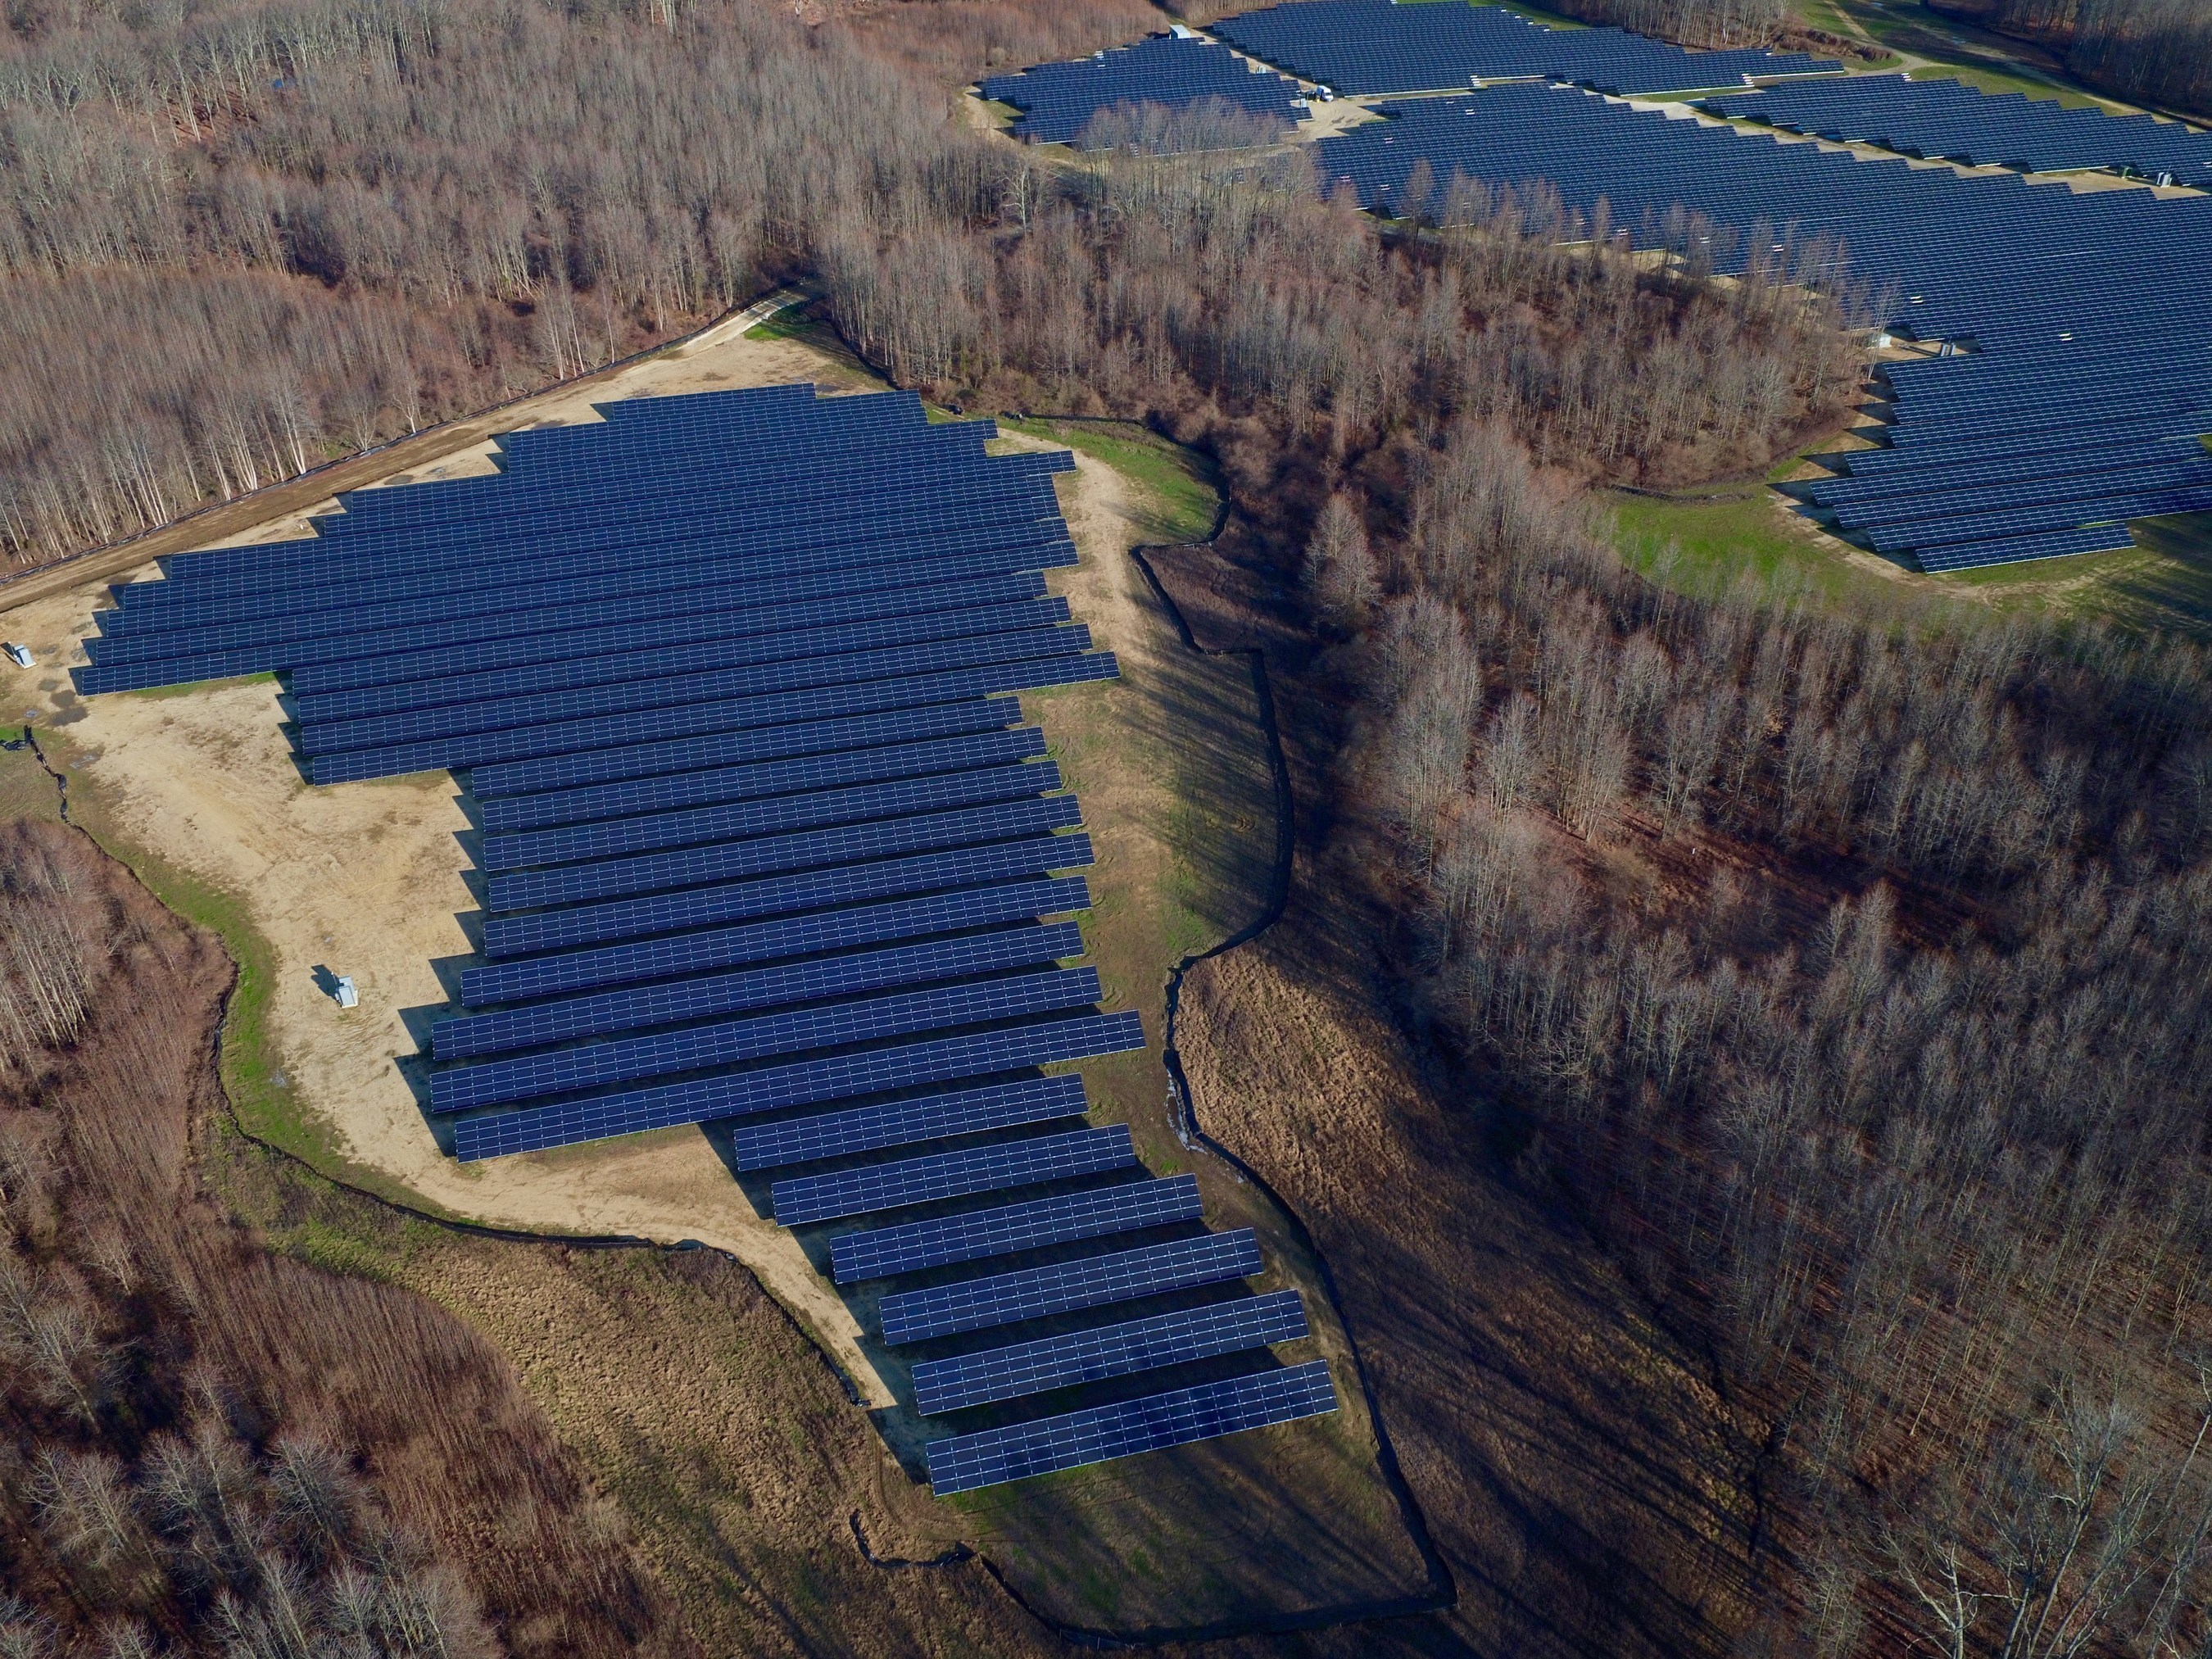
\includegraphics[width=0.8\textwidth]{figures/Problem/solarpark.jpg}
    \caption{12.8 MW Utility Project - the World's Largest Bifacial PV Installation in Eastern US}
	\label{fig:SolarPark}
\end{figure}
\todo[color=c01]{https://www.prnewswire.com/news-releases/sunpreme-deploys-the-worlds-largest-bifacial-pv-installation-for-a-128-mw-utility-project-in-eastern-us-300325989.html}
Commonly this is achieved by two devices,
a DC-DC boost converter (BC) to normalize the voltage
and an DC-AC inverter to generate AC power with the necessary frequency.

In this project we have a look at DC-DC boost converters.
The first part of the project is understanding and simulating common topologies.
The second part is understanding, simulating and building a new topology,
the 2NX Interleaved Boost Converter. \todo[color=c01]{Sanjee's paper is the source}


\section*{Reading Guide}
For readers without an understanding of DC-DC converters,
it is recommended to read the Chapters \ref{ch:basicI}-\ref{ch:basicII}, \todo[color=c01]{ref basic knowledge chapters}
before reading the Chapters \ref{ch:more_advancedI}-\ref{ch:more_advancedII}. \todo[color=c01]{ref advanced chapters}
as these require a deeper understanding.
\chapter{Problem Analysis}\label{ch:probdesc}



\section{Photovoltaic power}
While plants using fossil fuels or nuclear power are outputting high voltage AC directly into the grid, the renewable sources need to be boosted to high voltage, before they can feed their energy into the grid. 
Especially Solar panels produce very low DC-voltage. \cite{PanasonicSolarPanel}
%\todo[color=c01]{ref}
% https://panasonic.net/ecosolutions/solar/product/product_detail/index.html

The setup to supply the energy to the grid can be seen in Figure \ref{fig:SolarConverters}.
There are three stages between converting solar to electric power and inputting that power into the grid. 
First, the low voltage DC coming in from the panel needs to be boosted, before an inverter makes it alternating. Finally  an AC-AC converter 

This three steps involve complicated circuitry, large costs and significant power losses. 
This remains one of the big reasons why solar power is not as cost efficient as other sources that do not require such conversion.

\begin{figure}[H]
   \centering
   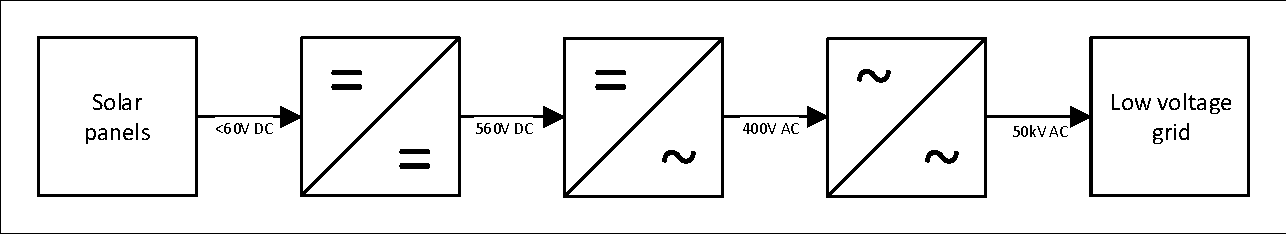
\includegraphics[width=\textwidth]{figures/Problem/SolarConverters.pdf}
    \caption{Connection of solar panels to the grid}
	\label{fig:SolarConverters}
\end{figure}

\section{Problem Description}
This project will focus on trying to improve the first stage or the DC-DC converter. 
The challenge for the boost converter is that the difference is very big.
A typical output of a solar panel is up to 60V DC while the low voltage grid is already 400V AC.
By connecting more panels in series a higher output voltage can be achieved but the power of individual panels can't be used as efficiently.
Using boost converters is the better solution but the standard boost converter topology is not suitable for this case. 
The maximum conversion ratio of the standard converter is limited to a ratio 7.7.
At least cascaded converters are needed to reach the higher internal voltage level.
But they still have to always run on high duty cycles to reach the demanded conversion ratios.
Advanced topologies have higher conversion ratios that may be useful for connecting solar panels.
In general new topologies for boost converters can have advantages over the conventional boost converters when it comes to compactness, efficiency and durability.

 

\section{Problem Definition}\label{sec:probdesc}
The goal of this report is to compare different DC-DC boost converter topologies and choose the one most suitable for PV appliances. The chosen circuit should be tested in both simulations and hardware. The comparison of the results to the requirements that will be set in Sections \ref{sec:req} will determine weather the project is a success. 

%Boosting DC power
%cheap
%size


\section{Requirements}\label{sec:req}
% maximum conversion ration higher than standard (7.7)
% No higher capacity/induction
% 22


\chapter{Development}\label{ch:dev}
\todo[color=c04,inline]{Development}
\section{Conventional Boost Converter}\label{ch:CBC}
\subsection{Principle of operation}\label{sec:CBC_POC}

The conventional boost converter uses one inductor,
one switch and one capacitor. When the switch is closed, the inductor current rises and energy is stored in the inductor L. When the switch is open, the inductor discharges through diode D and the inductor current falls. It steps up the voltage when
the switch is in OFF state. The two modes of operation will be discussed in this chapter. The circuit can be observed on figure~\ref{fig:CBC}. All the calculations in this chapter are based on \cite{Hart2010}.

\begin{figure}[H]
   \centering
   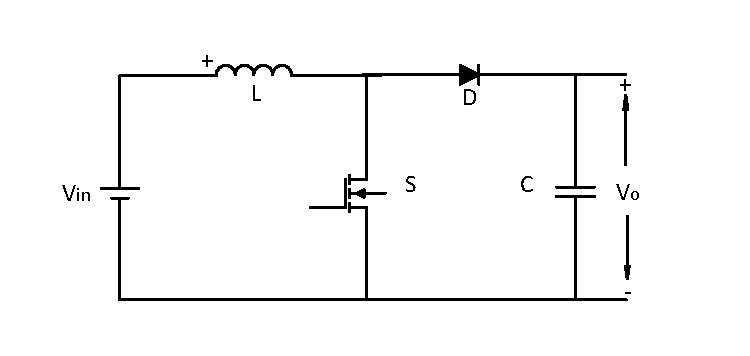
\includegraphics[width=0.8\textwidth]{figures/aConventionalBoost/ConventionalBoostConverter.pdf}
    \caption{Conventional Boost Converter}
	\label{fig:CBC}
\end{figure}

\subsection{Operation Modes}\label{sec:CBC_OP}

\subsubsection{Switch ON (Figure~\ref{fig:CBC_ON}):}

When the switch is ON,
the inductor is being charged and the capacitor discharges over the load resistor.

\begin{figure}[H]
   \centering
   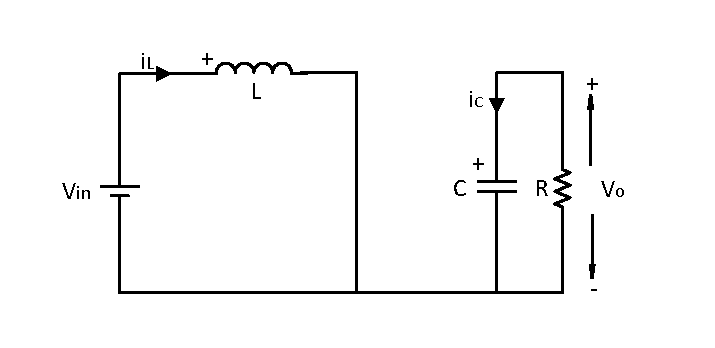
\includegraphics[width=0.8\textwidth]{figures/aConventionalBoost/ConventionalBoostConverterON.pdf}
    \caption{Conventional Boost Converter Switch ON}
	\label{fig:CBC_ON}
\end{figure}

In this case we have:
\begin{equation}
	V_L = V_{in}
	\label{eq:CBC_SWON1}
\end{equation}
where
\begin{equation}
	V_L = L \frac{di}{dt}
	\label{eq:CBC_SWON2}
\end{equation}
and
\begin{equation}
	V_C = V_R
	\label{eq:CBC_SWON3}
\end{equation}
The capacitor current discharges over the resistor:
\begin{equation}
	i_C = -\frac{V_o}{R}
	\label{eq:CBC_SWON4}
\end{equation}
\subsubsection{Switch OFF (Figure ~\ref{fig:CBC_OFF}):}

\begin{figure}[H]
   \centering
   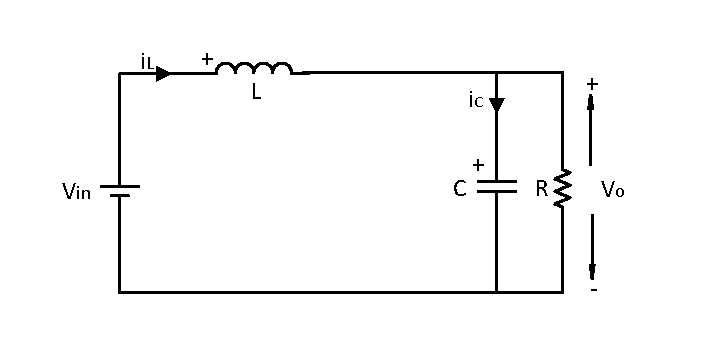
\includegraphics[width=0.8\textwidth]{figures/aConventionalBoost/ConventionalBoostConverterOFF.pdf}
    \caption{Conventional Boost Converter Switch OFF}
	\label{fig:CBC_OFF}
\end{figure}

When the switch is OFF,
the capacitor is being charged and this is the mode when the boosting happens.

In this case we have:
\begin{equation}
	V_L = V_{in} - V_o
	\label{eq:CBC_SWOFF1}
\end{equation}

\begin{equation}
	i_C = i_L -\frac{V_o}{R}
	\label{eq:CBC_SWOFF2}
\end{equation}

\begin{figure}[H]
   \centering
   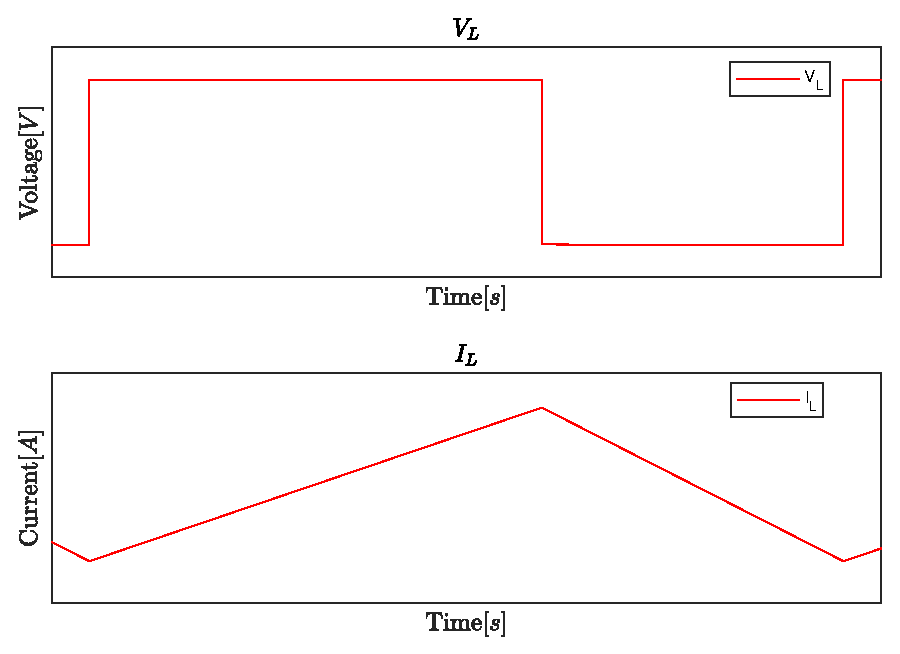
\includegraphics[width=0.8\textwidth]{figures/aConventionalBoost/LvAndLi.eps}
    \caption{CBC Inductor Wave Forms}
	\label{fig:CBC_InductorWaveForms}
\end{figure}

\subsection{Conversion ratio}\label{sec:conversionRatio}

Based on inductor volt-second balance, the conversion ratio can be calculated:

\begin{equation}
	\int_{0}^{T_s} v_L(t)dt = V_{in}D + (V_{in}-V_{out})(1-D) = 0
	\label{eq:CBC_VISB}
\end{equation}

\begin{equation}
	\frac{V_o}{V_{in}} = \frac{1}{1-D}
	\label{eq:CBC_CR}
\end{equation}

\subsection{Inductor current ripple}\label{sec:CBC_ICR}

The inductor current slope for the interval from 0 to $DT_s$ can be found as:

\begin{figure}[H]
   \centering
   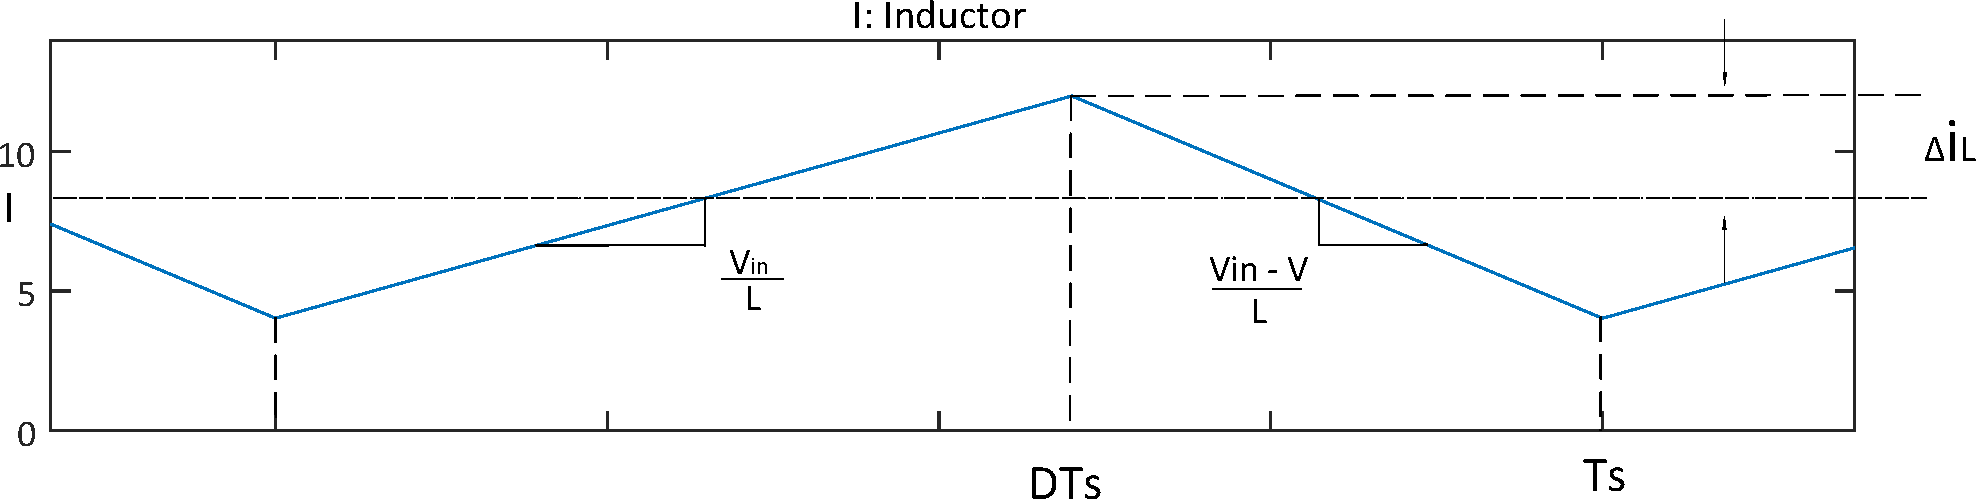
\includegraphics[width=\textwidth]{figures/aConventionalBoost/InductorCurrent.pdf}
    \caption{CBC Inductor Current Ripple}
	\label{fig:CBC_InductorCurrent}
\end{figure}


\begin{equation}
	\frac{di_L(t)}{dt} = \frac{v_L(t)}{L} = \frac{V_{in}}{L}
	\label{eq:CBC_ICR1}
\end{equation}

and the current slope for the interval (1 - DTs):

\begin{equation}
	\frac{di_L(t)}{dt} = \frac{v_L(t)}{L} = \frac{V_{in} - V}{L}
	\label{eq:CBC_ICR2}
\end{equation}

The change of inductor current during the first subinterval is:

\begin{equation}
	2\Delta i_L = \frac{V_{in}}{L}DT_s \Rightarrow
  \Delta i_L = \frac{V_{in}}{2L}DT_s
	\label{eq:CBC_ICR3}
\end{equation}

The inductor should be chosen such that a desired current ripple magnitude is optained.

\subsection{Capacitor voltage ripple}\label{sec:CBC_CVR}

\begin{figure}[H]
   \centering
   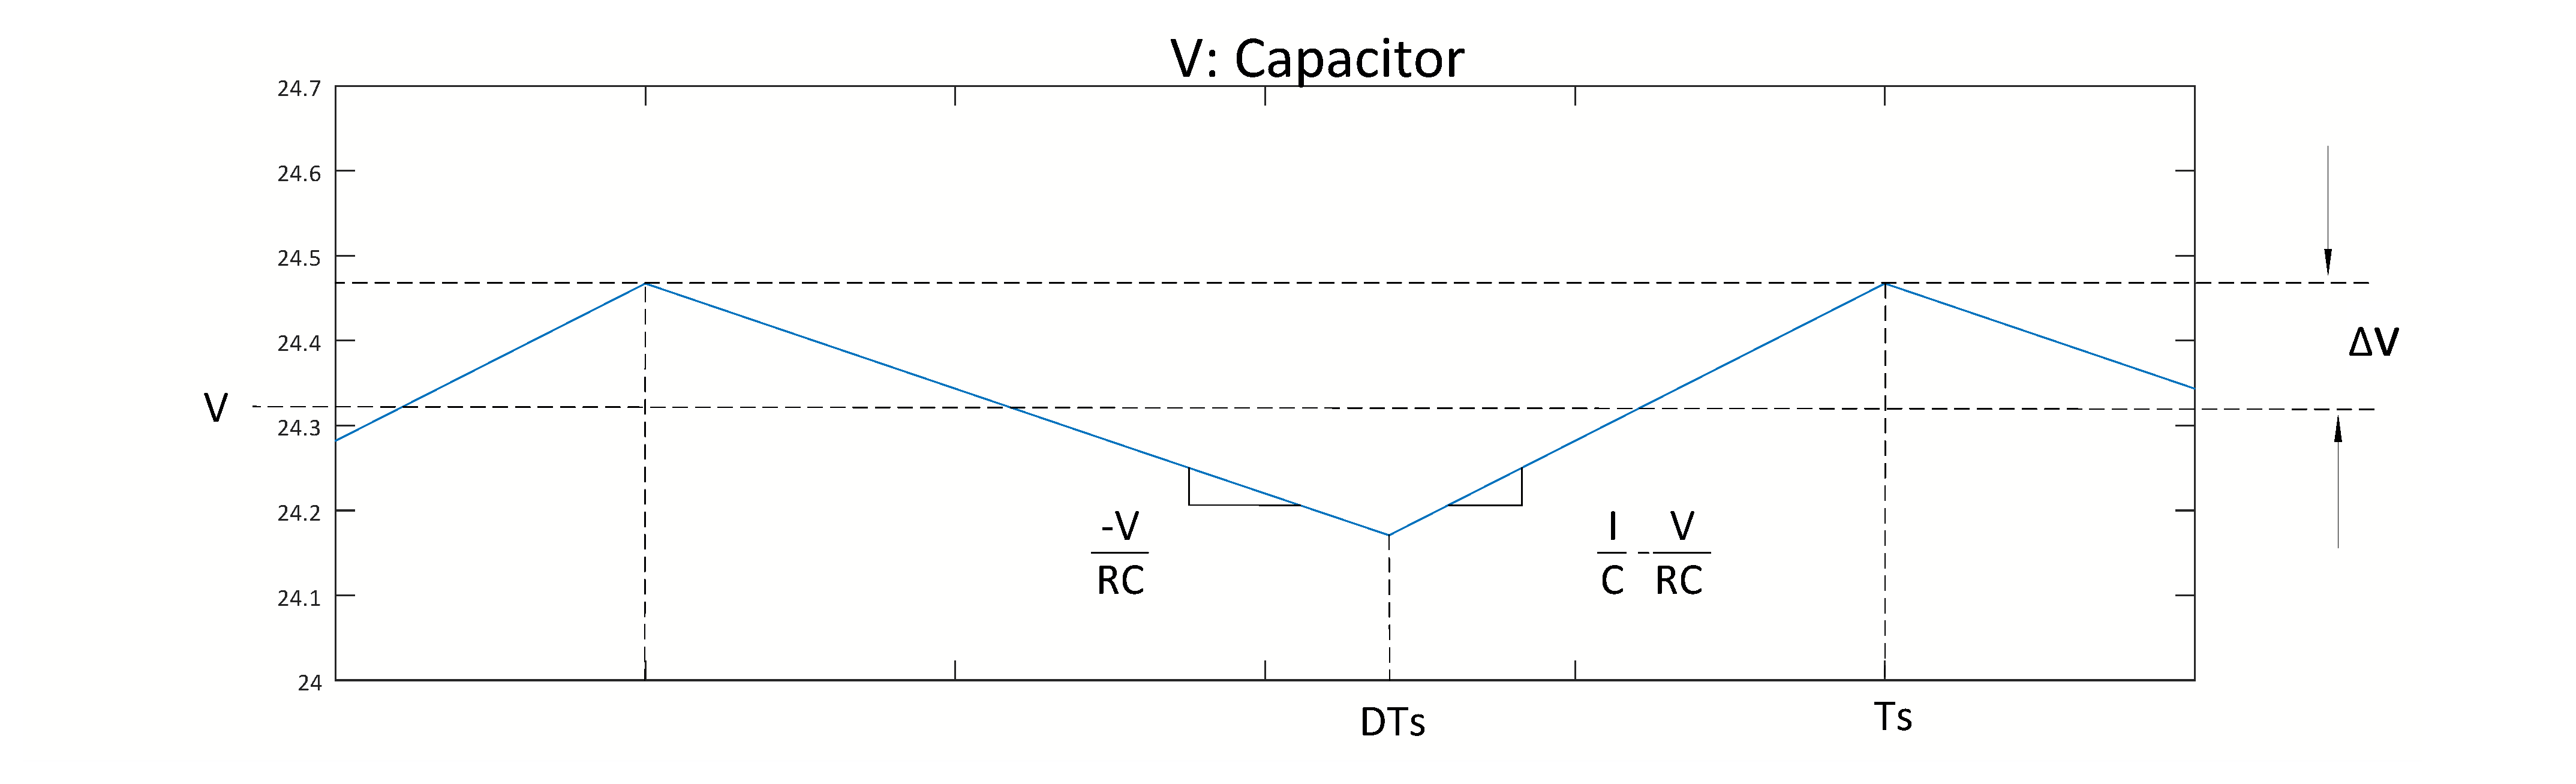
\includegraphics[width=\textwidth]{figures/aConventionalBoost/CapacitorVoltage.pdf}
    \caption{Capacitor Voltage Ripple}
	\label{fig:CBC_CVR1}
\end{figure}

The capacitor voltage slope for the interval from 0 to DTs can be found as:

\begin{equation}
	\frac{dv_c(t)}{dt} = \frac{i_c(t)}{C} = \frac{-V}{RC}
	\label{eq:CBC_CVR2}
\end{equation}

and the voltage slope for the interval (1 - DTs):

\begin{equation}
	\frac{dv_c(t)}{dt} = \frac{i_c(t)}{C} = \frac{I}{C} - \frac{V}{RC}
	\label{eq:CBC_CVR3}
\end{equation}

The change of capacitor voltage during the first subinterval is:

\begin{equation}
	-2\Delta v = \frac{-V}{RC}DT_s \Rightarrow
  \Delta v = \frac{V}{2RC}DT_s
	\label{eq:CBC_CVR4}
\end{equation}

The capacitor should be chosen according to the desired voltage ripple.

\subsection{Design Example}\label{sec:CBC_DE}

If we consider a design for a boost converter that will have an output of 25V from a 10V source, with a continuous inductor current and an output voltage of less than one percent, we will have the following parameters:\\
V\textsubscript{in} = 10 V, V\textsubscript{out} = 25 V and D = 0.6. Also,
a load resistor of 40 $\Omega$ and a  switching frequency of 25kHz are considered for the design.


By the fact that the average power supplied by the source must be the same as the average power absorbed by the load resistor, the output power can be obtained by:

\begin{equation}
	P_o = \frac{V^2_o}{R} = V_oI_o
	\label{eq:CBC_CVR4}
\end{equation}

and the input power is $V_{in}I_s = V_{in}I_L$

\begin{equation}
	\Rightarrow V_{in}I_L = \frac{V^2_o}{R} = \frac{[V_{in}/(1-D)]^2}{R}
	\label{eq:CBC_CVR4}
\end{equation}

solving for I\textsubscript{L}, we get:

\begin{equation}
	I_L = \frac{V_{in}}{(1-D)^2R}
	\label{eq:CBC_CVR4}
\end{equation}

The maximum and minimum inductor current can be determined by:

\begin{equation}
	I_{max} = I_L + \Delta i_L = \frac{V_{in}}{(1-D)^2R} + \frac{V_{in}DT_s}{2L}
	\label{eq:CBC_CVR4}
\end{equation}

\begin{equation}
	I_{min} = I_L - \Delta i_L = \frac{V_{in}}{(1-D)^2R} - \frac{V_{in}DT_s}{2L}
	\label{eq:CBC_CVR4}
\end{equation}


The induction current has to be continuous, so it has to be always positive. This means that I\textsubscript{L} has to be positive and the boundary between continuous and discontinuous inductor current is determined from:\\
\begin{equation}
	I_{min} = 0 = \frac{V_{in}}{(1-D)^2R} - \frac{V_{in}DT_s}{2L}
\end{equation}

\begin{equation}
	\frac{V_{in}}{(1-D)^2R} = \frac{V_{in}DT_s}{2L} = \frac{V_{in}D}{2Lf}
\end{equation}


So, the minimum combination of inductance and switching frequency for continuous current is:

\begin{equation}
L_{min} = \frac{D(1-D)^2R}{2f} = \frac{0.6(1-0.6)^2 40}{2\cdot25000} = 76.8\mu F
\end{equation}


L = 120 $\mu$F is selected to provide a margin to ensure continuous current.
Then, using Equation~\ref{eq:CBC_CVR4}, we can find the average inductor current.

\begin{equation}
I_L = \frac{V_{in}}{(1-D)^2R} = \frac{10}{(1-0.6)^2(40)} = 1.56 A
\end{equation}\\
Afterwards, the current ripple according to Figure~\ref{fig:CBC_InductorCurrent} is calculated using Equation~\ref{eq:CBC_CVR3}

\begin{equation}
\Delta i_L = \frac{V_{in}DT}{2L} = \frac{10\cdot 0.6}{2\cdot 100\cdot 10^{-6}\cdot 25000} = 1 A
\end{equation}\\
$I_{max} = 1.56 + 1 = 2.56 A$ , 
$I_{min} = 1.56 - 1 = 0.56 A$


Based on equation ~\ref{eq:CBC_CVR4}, the minimum capacitance required to limit the output voltage ripple to 1 percent is:

\begin{equation}
C_{min} = \frac{D}{R(\Delta V_o/V)f} = \frac{0.6}{40\cdot 0.01\cdot 25000 } = 60\mu F
\end{equation}\\
A capacitor of 80 $\mu$ F was chosen to provide a satisfactory margin.\\

To confirm the calculations, the circuit was built in SIMULINK, using the calculated parameters presented on Table~\ref{tab:CBC}.

\begin{table}[H]
\begin{center}
\caption {Simulation parameters for CBC} \label{tab:CBC} 
\begin{tabular}{|l|l|}
\cline{1-2}
\textbf{Parameter} & \textbf{Value}  \\ \cline{1-2}
Input Voltage $V_{in}$          &      10V   \\ \cline{1-2}
Load(R)   & 40$\Omega$           \\ \cline{1-2}
Capacitance(C)          &       80$\mu$F     \\ \cline{1-2}
Inductance(L)          &      120$\mu$F      \\ \cline{1-2}
Duty cycle(D)          &     0.6       \\ \cline{1-2}
Switching Frequency($f$)          &      25kHz      \\ \cline{1-2}
\end{tabular}
\end{center}
\end{table}

The simulation presented on Figure~\ref{fig:CBC_Sim} is using an ideal switch for the active device.

\begin{figure}[H]
   \centering
   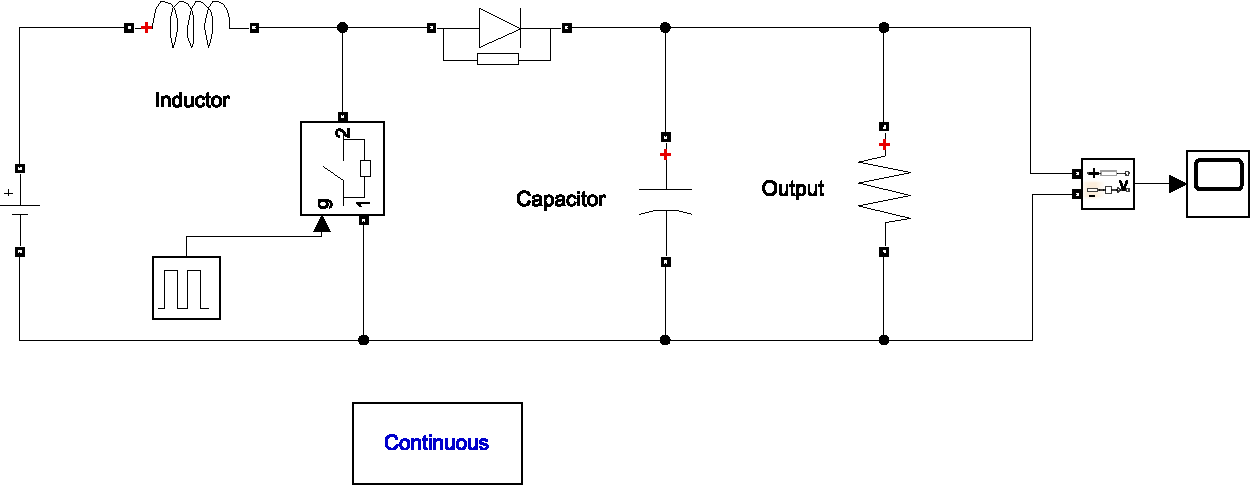
\includegraphics[width=0.8\textwidth]{figures/aConventionalBoost/CBCpic.pdf}
    \caption{Conventional Boost Converter}
	\label{fig:CBC_Sim}
\end{figure}

The results from the simulation are presented on Figure~\ref{fig:CBC_SimResults} and it can be observed that they match with the calculations. 

\begin{figure}[H]%
    \centering
    %\subfloat[Switch ON\label{SI_ON}]
    {{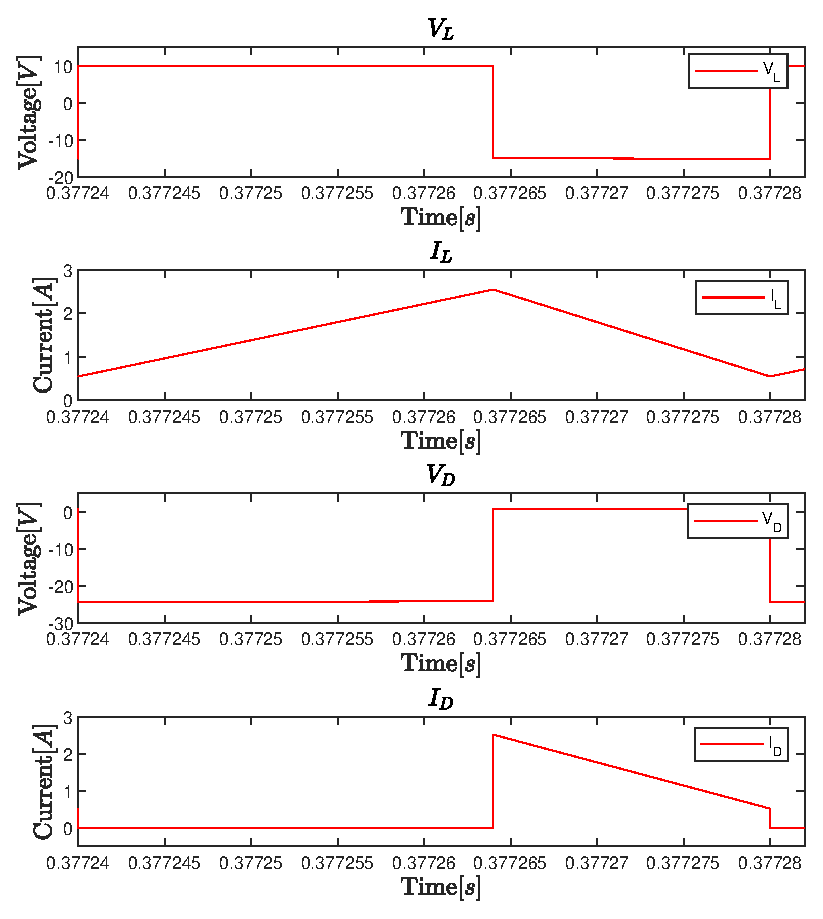
\includegraphics[width=0.8\textwidth]{figures/aConventionalBoost/CBC_V_LtoI_D.eps} }}%
    \qquad
    \subfloat{{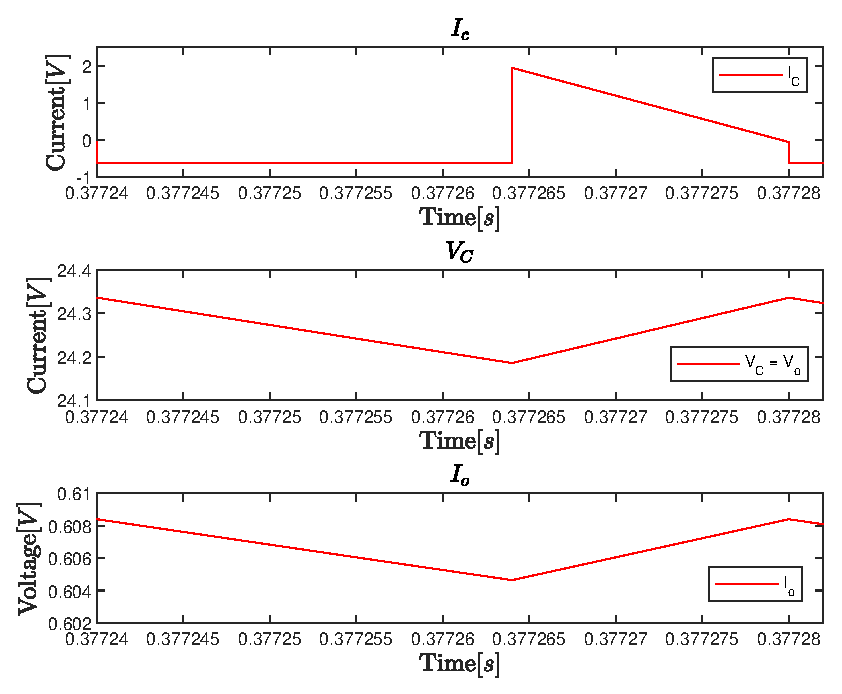
\includegraphics[width=0.8\textwidth]{figures/aConventionalBoost/CBC_I_CtoI_out.eps} }}%  
    \caption{Simulation results}%
     \label{fig:CBC_SimResults}% 
\end{figure}
section{Topology Comparison}

\section{Switched Inductor}\label{ch:SIBC}
The Switched Inductor Boost Converter (SIBC) is a small alternation to the Conventional Boost Converter mentioned in Chapter \ref{ch:CBC}.
It only adds passive components to an already known topology,
which means the same switching scheme can be used.
\subsection{Additions from Conventional BC}
In the SIBC,
the single inductor from the Conventional BC gets replaced by two inductors and three diodes,
connected as shown in Figure \ref{fig:SwitchedInductor}.

\begin{figure}
   \centering
   \includegraphics[width=\textwidth]{figures/bSwitchedInductor/switched_inductor.pdf}
    \caption{Switched inductor boost converter circuit}
	\label{fig:SwitchedInductor}
\end{figure}


With this configuration,
the inductors form two different topologies during the ON and OFF states. By reversing the biasing of the diodes the inductors are connected in parallel during ON state and series during OFF state.  \todo[color=c04b]{refer to figure maybe} 


\subsection{Switching States}
The same switching scheme as for the Conventional BC can be used,
as mentioned earlier.
The equivalent circuits during the on and off stage are shown in Figure \ref{fig:SI_States}.

\begin{figure}[H]%
    \centering
    \subfloat[Switch ON\label{SI_ON}]
    {{\includegraphics[width=6.5cm]{figures/bSwitchedInductor/switched_inductorON.pdf} }}%
    \qquad
    \subfloat[Switch OFF\label{SI_OFF}]{{\includegraphics[width=6.5cm]{figures/bSwitchedInductor/switched_inductorOFF.pdf} }}%  
    \caption{Switching states of the SIBC}%
     \label{fig:SI_States}% 
\end{figure}

\subsubsection{ON State}
While the switch is ON, diodes D\textsubscript{1} and D\textsubscript{2} are forward biased and diode ? is reverse biased.
This constructs a parallel conection between the inductors, as seen in Figure \ref{SI_ON}.
\\*
In this case, we can use KVL to build the eqation: 

\begin{equation}
	V_L=V_{in}
	\label{eq:SI_KVL_ON}
\end{equation}

\subsubsection{OFF State}
While the switch is OFF, the complete opposite happens, where only D\textsubscript{2} remains forward biased and forms a series connections between the inductors (shown on Figure \ref{SI_OFF}).
In a configuration like this we can assume equal split of the pottential across the inductors and using KVL construct the equation:
\begin{equation}
	V_{in}-2V_L-V_o=0
	\label{eq:SI_KVL_OFF}
\end{equation}
Subsequetially reformed as:
\begin{equation}
	V_L=\frac{V_{in} - V_o}{2}
	\label{eq:SI_KVL_OFF2}
\end{equation}
 \\*
Reforming the Inductor voltage-second balance(Explained in Sections \ref{sec:convertionRatio} for the current topology, we get the following relationship:

\begin{equation}
	V_{L(ON)}D+V_{L(OFF)}(1-D)=0
	\label{eq:SI_IVSB}
\end{equation}
Substituting the already derived expressions for V\textsubscript{L}:
\begin{equation}
	V_{in}D+\frac{V_{in} - V_o}{2}(1-D)=0
	\label{eq:SI_IVSB2}
\end{equation}
Subsequenlty the input/output relationship can be stated as:

\begin{equation}
	\frac{V_o}{V_{in}} = \frac{1+D}{1-D}
	\label{eq:pumpHeadMode5}
\end{equation}


%\subsection{Single Switch Quadratic BC}\label{ch:SSQBC}
\todo[color=c04c,inline]{testing the colors}
%\section{Conventional Three Level Boost Converter}\label{ch:TLBC}

The conventional three level boost converter is the first variation of the conventional BC that includes not only passive components, but also an additional active component. This, as in all other topologies discussed, increases the ratio between output and input, this time in a completely linear manner, as it will be proven in the this section. 

\subsection{Additions from Conventional BC}
In the CTLBC, a second switch is included, together with another capacitor to go in parallel with it, An additional diode is included to allow both switches to conduct at the same time without causing damage to the circuit.The full schematic can be seen on Fig. \ref{fig:CTLBC}  

\begin{figure} [H]
   \centering
   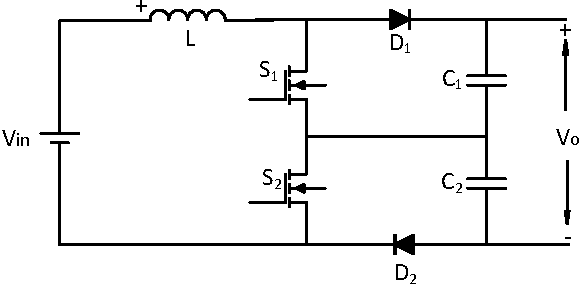
\includegraphics[width=0.6\textwidth]{figures/dConventionalThreeLevelBC/Three_level.pdf}
    \caption{Conventional Three Level Boost Converter circuit}
	\label{fig:CTLBC}
\end{figure}
\subsection{Switching States}
As there are two switches in this topology, a different switching pattern is required in comparison to the Conventional BC. The pattern of choice is shifting the signal to the second switch by The angle is 90$^\circ$ degrees.
In this case, there are four possible states, corresponding to all possible combinations between the switches. Not all of them occur for one given duty cycle value. 
The equivalent circuits during the on and off stages are shown in Figure \ref{fig:CTLBC_States}. Here again we assume the capacitors are the same size and that the duty ratio applied to the two switches is the same. 
\vspace{-5mm}
\begin{figure}[H]%
    \centering
    \subfloat[Switch S\textsubscript{1} ON, Switch S\textsubscript{2} ON\label{CTLBC_ONON}]
    {{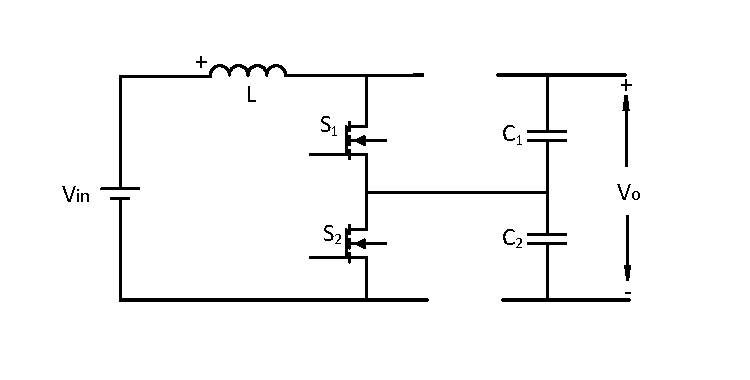
\includegraphics[width=0.45\textwidth]{figures/dConventionalThreeLevelBC/Three_levelONON.pdf} }}%
    \qquad
    \subfloat[Switch S\textsubscript{1} ON, Switch S\textsubscript{2} OFF\label{CTLBC_ONOFF}]{{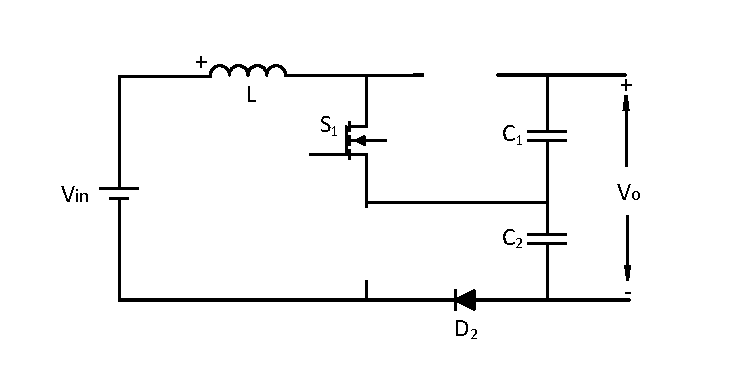
\includegraphics[width=0.45\textwidth]{figures/dConventionalThreeLevelBC/Three_levelONOFF.pdf} }}%  
   \qquad
        \subfloat[Switch S\textsubscript{1} OFF, Switch S\textsubscript{2} ON\label{CTLBC_OFFON}]
    {{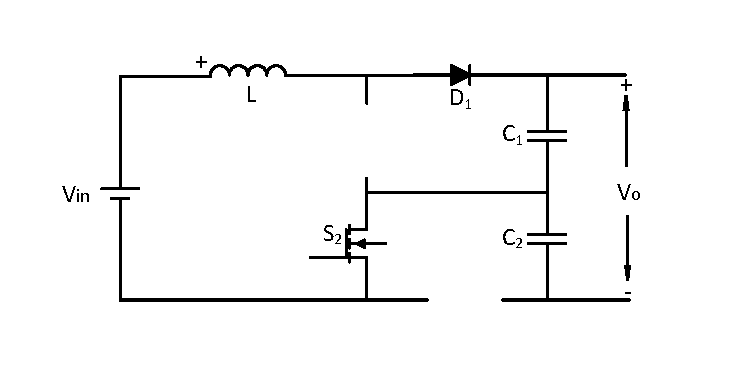
\includegraphics[width=0.45\textwidth]{figures/dConventionalThreeLevelBC/Three_levelOFFON.pdf} }}%
    \qquad
    \subfloat[Switch S\textsubscript{1} OFF, Switch S\textsubscript{2} OFF\label{CTLBC_OFFOFF}]{{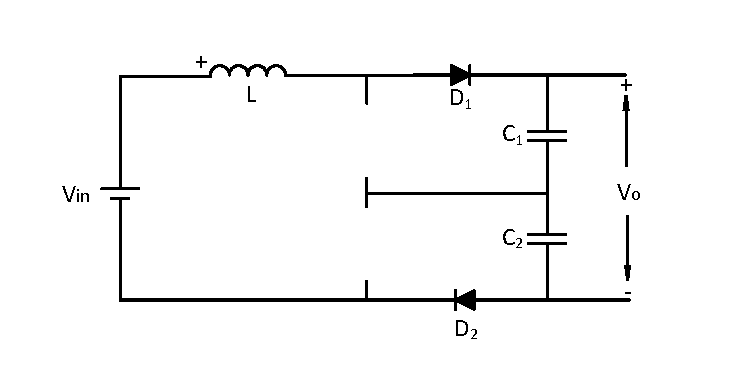
\includegraphics[width=0.45\textwidth]{figures/dConventionalThreeLevelBC/Three_levelOFFOFF.pdf} }}%  
    \caption{Switching states of the SIBC}%
     \label{fig:CTLBC_States}% 
     
\end{figure}
\subsubsection{Switch S\textsubscript{1} ON, Switch S\textsubscript{2} ON State}
Here we have got a replica of the ON state of a conventional boost converter, as both switches conduct and both diodes are reverse biased.(Can be seen on Figure \ref{CTLBC_ONON}) A loop is formed with the inductor and the power supply. We use KVL to express the voltage over the inductor as: 

\begin{equation}
	V_{L}=V_{in}
	\label{eq:CTLBC_KVL_ONON}
\end{equation}
Another loop is formed with the two capacitor and the output.This loop can be observed over all the rest of the states as well. Again assuming the capacitors are the same size, the voltage would split equally across them and the loop can be expressed via KVL as: 

\begin{equation}
	V_O=2V_C
	\label{eq:CTLBC_KVL_ONON2}
\end{equation}


\subsubsection{Switch S\textsubscript{1} ON, Switch S\textsubscript{2} OFF State}
While only switch S\textsubscript{1}conducts, diode D\textsubscript{2} is forwards biased and extends the loop over C\textsubscript{2}.(Can be seen on Figure \ref{CTLBC_ONOFF}) We use KVL to express the voltage over the inductor as: 
\begin{equation}
	V_{L}=V_{in}-V_C
	\label{eq:CTLBC_KVL_ONOFF}
\end{equation}
 
\subsubsection{Switch S\textsubscript{1} OFF, Switch S\textsubscript{2} ON State}
Similar to the previous state, S\textsubscript{2}conducts, diode D\textsubscript{1} is forwards biased and extends the loop over C\textsubscript{1} (Can be seen on Figure \ref{CTLBC_OFFON}). As already stated, capacitor sizes and duty cycles are assumed equal, therefore no change in KVL between the two loops: 
\begin{equation}
	V_{L}=V_{in}-V_C
	\label{eq:CTLBC_KVL_OFFON}
\end{equation}

\subsubsection{Switch S\textsubscript{1} OFF, Switch S\textsubscript{2} OFF State}
With both switches open the circuit formed is equivalent to the OFF state in a conventional BC.(Can be seen on Figure \ref{CTLBC_OFFOFF}) We use KVL to express the voltage over the inductor as: 
\begin{equation}
	V_{L}=V_{in}-V_{O}
	\label{eq:CTLBC_KVL_OFFOFF}
\end{equation}

To find an expression for the output-input gain of the topology, we refer back to the IVSB (Sec. \ref{sec:convertionRatio})and formulate the expression that is valid for both switches since Eq. \ref{eq:CTLBC_KVL_ONOFF} and Eq.\ref{eq:CTLBC_KVL_OFFON} are identical:
\begin{equation}
	V_{L(ON)}D+V_{L(OFF)}(1-D)=0
	\label{eq:CTLBC_IVSB}
\end{equation}
Substituting the already derived expressions for V\textsubscript{L}:

\begin{equation}
	V_{in}D+(V_{in} - V_C)(1-D)=0
	\label{eq:CTLBC_IVSB2}
\end{equation}
Reforming this equation we get: 
\begin{equation}
	V_{in}=V_C(1-D)
	\label{eq:CTLBC_IVSB3}
\end{equation}
Using the already derived expression for V\textsubscript{O} in Eq.\ref{eq:CTLBC_KVL_ONON2} we can directly form the output-input function: 
\begin{equation}
	\frac{V_O}{V_{in}}=\frac{2}{(1-D)}
	\label{eq:CTLBC_IVSB4}
\end{equation}
Otherwise expressed, the gain of the CTLBC is twice the one of a conventional BC. 
\todo[color=c04,inline]{Add simulation results}
%\section{Cockroft Walton}\label{ch:cock}
\todo[color=c04x,inline]{testing the colors}
%\section{Non-inverting Nx Multilevel BC}\label{ch:MBC}

\todo[color=c04y,inline]{testing the colors}

Adding Cockcroft Walton Multiplier explained in Chapter~\ref{ch:cock} with a Conventional Boost Converter (Chapter~\ref{ch:CBC}), we get the Non-inverting Nx Multilevel Boost Converter as shown on Figure~\ref{fig:MBC_CW_CBCtoNx}. \cite{Bhaskar2016}

\begin{figure}[H]
   \centering
   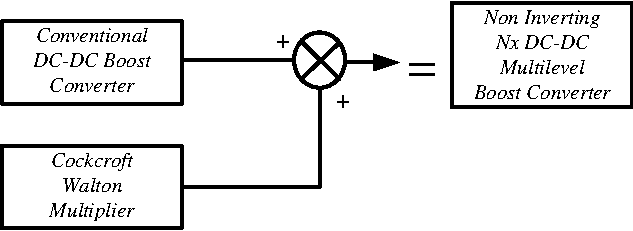
\includegraphics[width=\textwidth]{figures/yMultilevel/CW_CBCtoNx.pdf}
   \caption{Inverting Nx MBC Diagram}
	\label{fig:MBC_CW_CBCtoNx}
\end{figure}


The Non-inverting Nx Multilevel Boost Converter (Figure~\ref{fig:MBC_3XFULL}) is based on one switching device, 2N - 1 diodes and 2N - 1 capacitors, where N indicates the level number of the converter and can be extended by adding capacitors and diodes while the main circuit is not required to be changed. \cite{Rosas-Caro2008}

\begin{figure}[H]
   \centering
   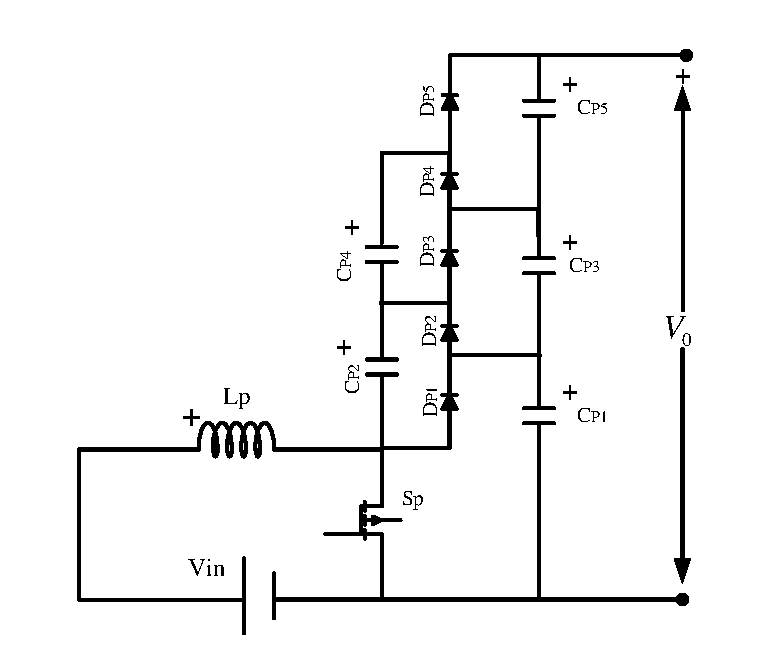
\includegraphics[width=\textwidth]{figures/yMultilevel/3x_FULL.pdf}
    \caption{Nx Multilevel Boost Converter}
	\label{fig:MBC_3XFULL}
\end{figure}

\subsection{Additions from Conventional BC}
The first part of the converter is the conventional DC-DC boost converter described in Chapter~\ref{ch:CBC}. The difference between the two converters is that the output of the multilevel converter is $V_C$ multiplied by the number of levels N, so that a higher output - input voltage ratio can be achieved. The example on Figure~\ref{fig:MBC_3XFULL} is a three-level converter, which means that the output voltage will equal to $3V_{Cp1}$. 

\subsection{Switching States}
The switching modes are the same as a Conventional BC. Like the other topologies mentioned on the previous pages, we assume that the size of all inductors and capacitors is the same. The corresponding circuits for ON and OFF states are displayed on Figure~\ref{fig:MBC_States} and they are based on \cite{Rosas-Caro2008}.

\begin{figure}[H]%
    \centering
    \subfloat[Switch ON\label{MBC_ON}]
    {{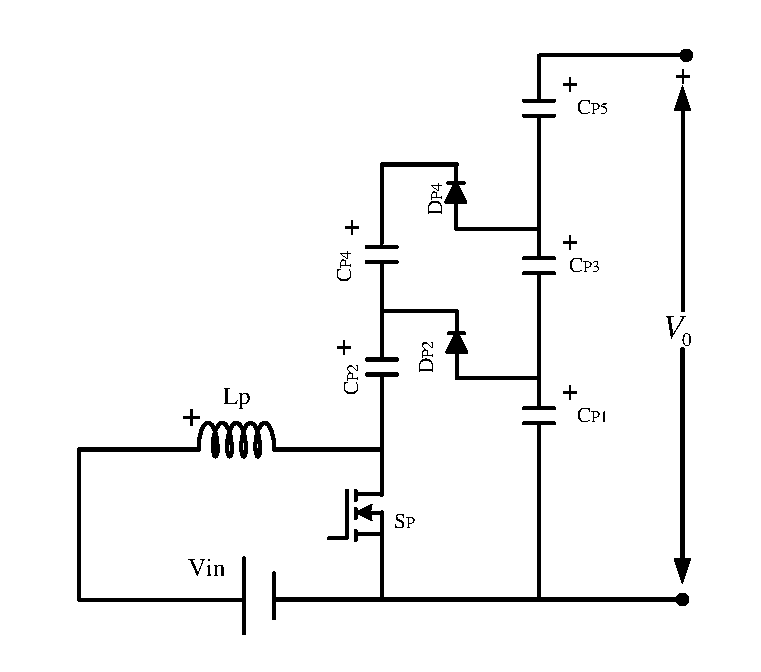
\includegraphics[width=0.45\textwidth]{figures/yMultiLevel/3x_ON.pdf} }}%
    \qquad
    \subfloat[Switch OFF\label{MBC_OFF}]{{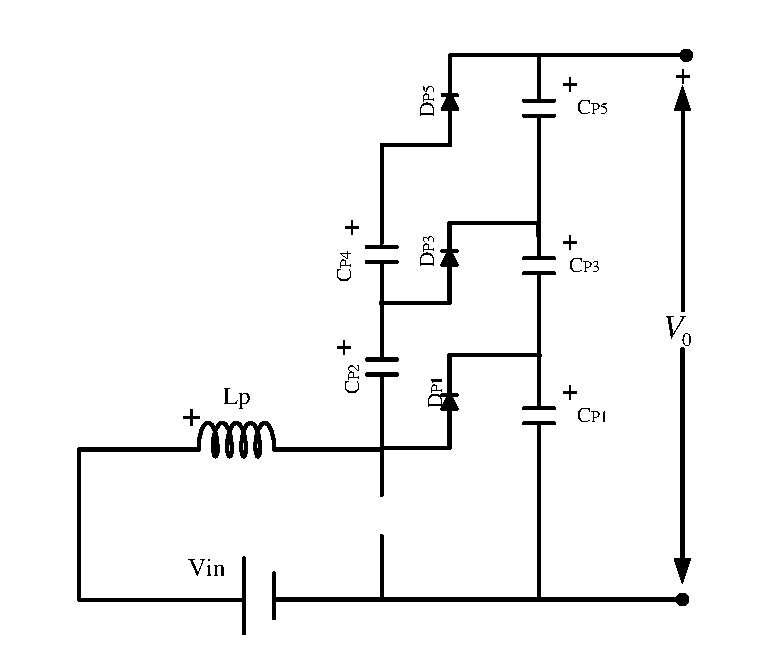
\includegraphics[width=0.45\textwidth]{figures/yMultiLevel/3x_OFF.pdf} }}%  
    \caption{Switching states of the MBC}%
     \label{fig:MBC_States}% 
\end{figure}


\subsubsection{ON State}

During the ON state, $L_p$ is charged by the voltage source. If the voltage across $C_{P1}$ is higher then $C_{P2}$, the capacitor $C_{P1}$ clamps $C_{P2}$ through $D_{P2}$. At the same time, if the voltage across $C_{P2}$ + $C_{P4}$ is smaller than $C_{P1}$ + $C_{P3}$, then the capacitor $C_{P1}$ and $C_{P3}$ clamp the voltage across $C_{P2}$ and $C_{P4}$ through $D_{P4}$ and $C_{P4}$ is clamped by $C_{P3}$. The equations for when the switch is in ON position are as follows:

\begin{equation}
	V_L = V_{in} 
	\label{eq:MBC_ON1}
\end{equation} 

\begin{equation}
	V_{Cp1} = V_{Cp2} = V_{Cp3} = V_{Cp4}
	\label{eq:MBC_ON2}
\end{equation} 

\begin{equation}
	V_{Cp1} + V_{Cp4} = V_{Cp1} + V_{Cp3}
	\label{eq:MBC_ON3}
\end{equation} 

\begin{equation}
	V_o = V_{Cp1} + V_{Cp3} + V_{Cp5} = 3V_{Cp1}
	\label{eq:MBC_ON4}
\end{equation}

\subsubsection{OFF State}
When the switch is open, the inductor is in discharge mode and is charging capacitor $C_{P1}$ through diode $D_{P1}$. At this time $V_{in}$, $V_{Lp}$ and $C_{P2}$ clamp the voltage across $C_{P1}$ and $C_{P3}$ through diode $D_{P3}$. In the same manner, the input voltage $V_{in}$, the inductor voltage $V_{Lp}$, the voltage across $C_{P2}$ and $C_{P4}$ clamp the voltage across $C_{P1}$, $C_{P3}$ and $C_{P5}$.

The equations for the off state of the switch are as follows:

\begin{equation}
	V_L = V_{in} - V_{Cp1}
	\label{eq:MBC_OFF1}
\end{equation}

\begin{equation}
	V_{Cp1} + V_{Cp3} = V_{in} - V{L} + V_{Cp2}
	\label{eq:MBC_OFF2}
\end{equation}
 
\begin{equation}
	V_{Cp1} + V_{Cp3} + V_{Cp5} = V_{in} - V{L} + V_{Cp2} + V_{Cp4}
	\label{eq:MBC_OFF3}
\end{equation}

\begin{equation}
	V_{Cp1} + V_{Cp3} + V_{Cp5} = V_o
	\label{eq:MBC_OFF4}
\end{equation}

\subsection{Conversion Ratio}

To find the conversion ratio of this converter we can use the Inductor voltage-second balance as follows:

\begin{equation}
	V_{in}D + V_{in}(1-D) - V_{Cp1}(1-D)= 0 
	\Rightarrow
	V_{in} = V_{Cp1}(1-D)
	\label{eq:MBC_INVSB1}
\end{equation}

From Equations~\ref{eq:MBC_ON4} and~\ref{eq:MBC_INVSB1}, output-input voltage relationship is:
\begin{equation}
	\frac{V_o}{V_{in}} = \frac{3V_{Cp1}}{V_{Cp1}(1-D)} = \frac{3}{(1-D)}
	\label{eq:MBC_INVSB2}
\end{equation}

From here, we can generalize the conversion ratio for a Nx Multilevel Boost Converter as:
\begin{equation}
	\frac{V_o}{V_{in}} = \frac{N}{(1-D)}
	\label{eq:MBC_INVSB3}
\end{equation}

\subsection{Simulation results}

To confirm the calculations, the circuit was simulated in SIMULINK, using the following parameters: 

\begin{table}[H]
\begin{center}
\caption {Simulation parameters for MBC} \label{tab:MBC} 
\begin{tabular}{|l|l|}
\cline{1-2}
\textbf{Parameter} & \textbf{Value}  \\ \cline{1-2}
Input Voltage $V_{in}$          &      10V   \\ \cline{1-2}
Load(R)   & 225$\Omega$           \\ \cline{1-2}
Capacitance(C)          &       220$\mu$F     \\ \cline{1-2}
Inductance(L)          &      150$\mu$F      \\ \cline{1-2}
Duty cycle(D)          &     0.6       \\ \cline{1-2}
Switching Frequency($F_S$)          &      50kHz      \\ \cline{1-2}
\end{tabular}
\end{center}
\end{table}

The  topology was modelled with the listed values Figure.\ref{fig:MBC_Sim}. As the previous topologies presented, the components were assumed ideal.

\begin{figure}[H]
   \centering
   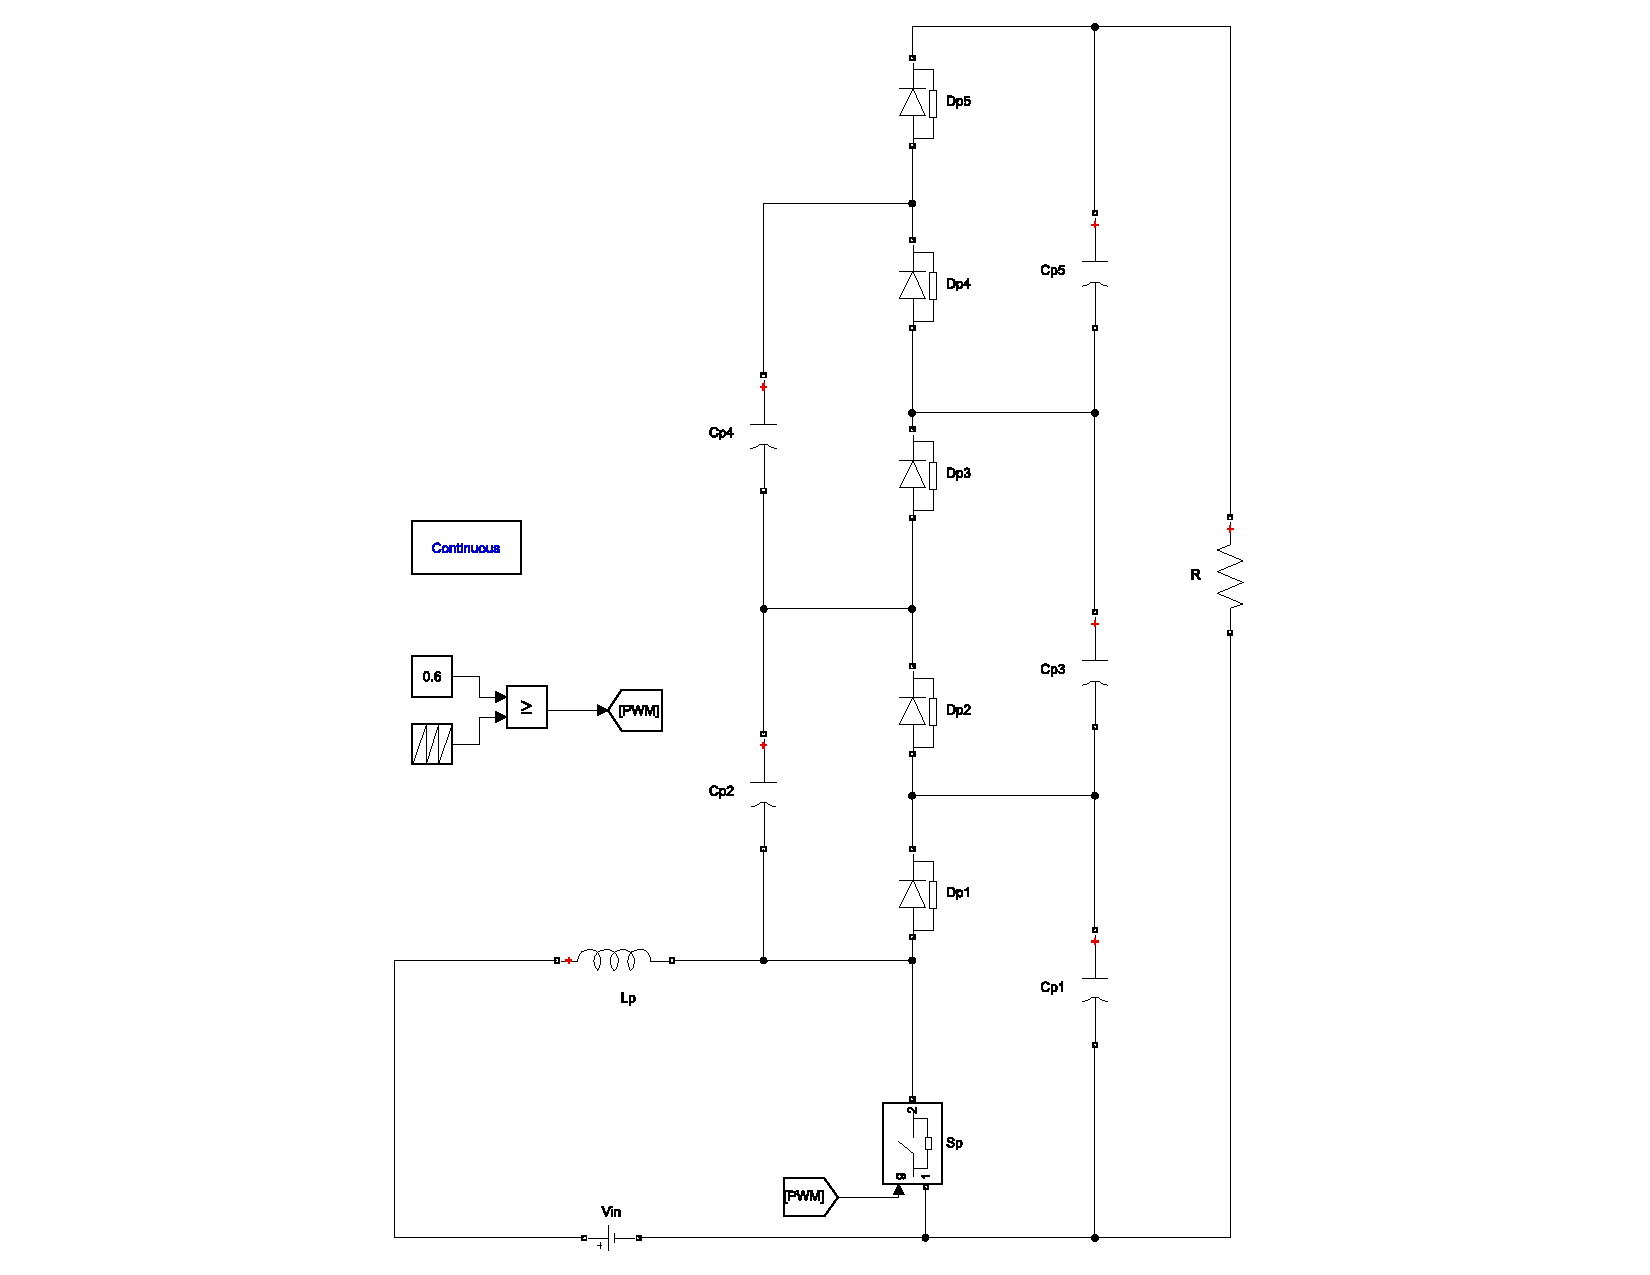
\includegraphics[width=\textwidth]{figures/yMultilevel/MCB_Simulation.pdf}
    \caption{Nx Multilevel Boost Converter Simulation}
	\label{fig:MBC_Sim}
\end{figure}

For the three level boost converter, the voltage gain for 0.6 duty cycle is 7.5. Running the simulation, we get the corresponding result of 75V as observed on Figure~\ref{fig:MBC_SimResults}.

\begin{figure}[H]
   \centering
   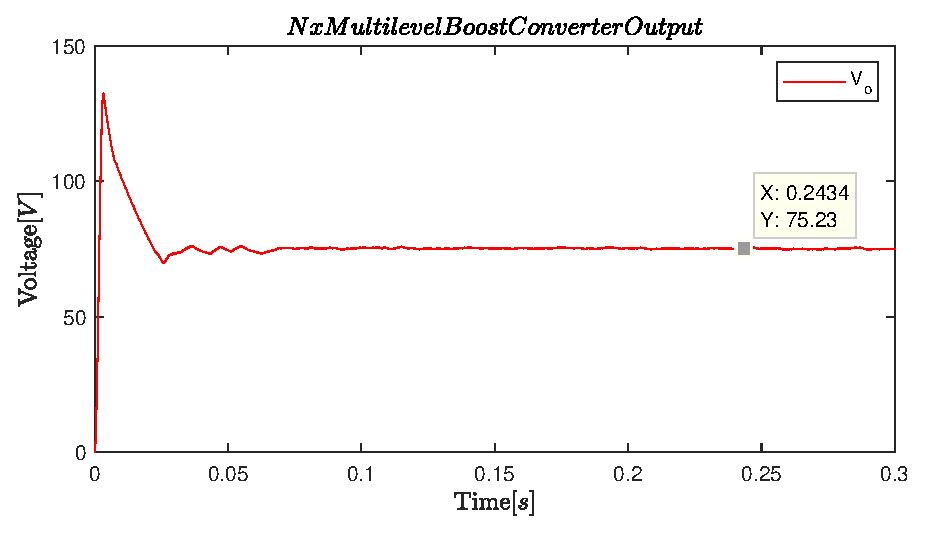
\includegraphics[width=\textwidth]{figures/yMultilevel/Non-invertingNx.eps}
    \caption{Nx Multilevel Boost Converter Simulation Results}
	\label{fig:MBC_SimResults}
\end{figure}

\section{Inverting Nx Multilevel BC}\label{ch:IMBC}

The Inverting Nx Multilevel Boost Converter can be achieved similar to the non-inverting one, but this time the Cockcroft Walton Multiplier is substracted as shown on Figure~\ref{fig:MBC_CW_CBCtoINx}. \cite{Bhaskar2016}

\begin{figure}[H]
   \centering
   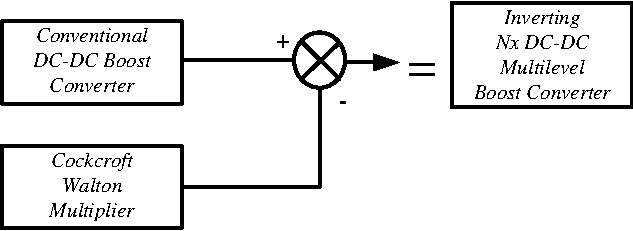
\includegraphics[width=\textwidth]{figures/yMultilevel/InvertingNxDiagram.pdf}
    \caption{Inverting Nx MBC Diagram}
	\label{fig:MBC_CW_CBCtoINx}
\end{figure}

The switching states equations and the conversion ratio are not derived as they are the same as the non-inverting Nx Multilevel Boost Converter. The main difference between the two converters is that additional diode and a capacitor are added as well as the diodes are reversed, so that the output voltage becomes with a negative sign as shown on Figure~\ref{fig:MBC_InvertingNx}.

\begin{figure}[H]
   \centering
   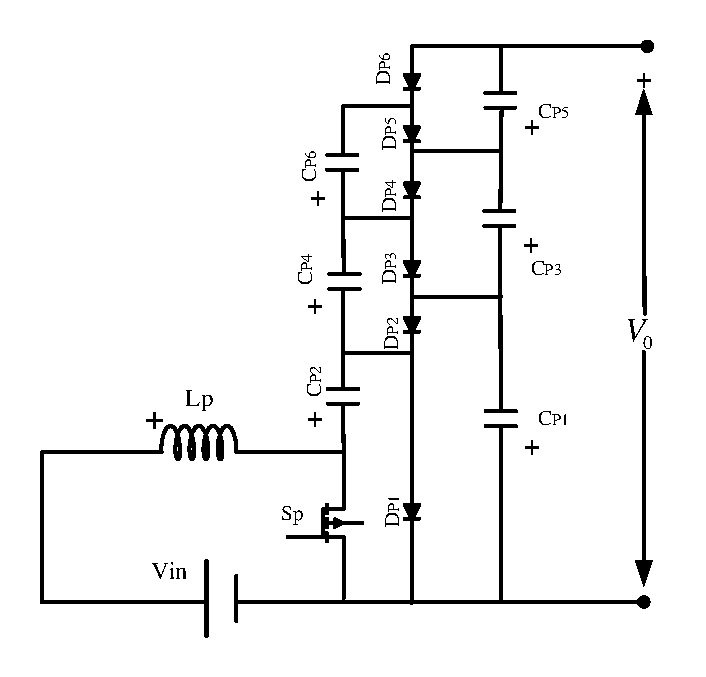
\includegraphics[width=\textwidth]{figures/yMultilevel/InvertingMBCforReport2.pdf}
    \caption{Inverting Nx MBC Schematic}
	\label{fig:MBC_InvertingNx}
\end{figure}


	
\chapter{Implementation}\label{ch:implement}

\section{Component Specifications}\label{ch:compSpec}
\todo[color=c05a,inline]{testing the colors}

\subsection{MOSFETs}
For the circuit the MOSFET C2M0160120D from Wolfspeed/Cree was chosen. 
It features a high blocking voltage, low on-resistance and low capacity.
That means it is able to work efficiently in high frequency power applications with small losses in switching, making it very suitable for converters.

The MOSFET is rated for switching voltages up to 1200V with a maximum current of 19A.
For switching a gate voltage of 14V is required and a negative input of -5V to -10V as a low input is recommended for fast switching.

\subsection{Diodes}
The used diode is the STTH6012 from STMicroelectronics.
The ultra fast soft recovery characteristics make it very efficient in high frequency pulse operation.
With a rating of 1200V repetitive peak reverse voltage and a maximum forward current of 60A the diode seems oversized but for experimental work they were used.

\subsection{Capacitors}
The chosen capacitors are standard sizes of $2.2 \mu F$ capacity with a voltage rating to 450V.

\subsection{Inductors}
%The inductor was winded by hand over a
\todo[color=c05a,inline]{missing}
\vspace{-8mm}
\section{Driver}\label{sec:driver}
\vspace{-3mm}
To control the MOSFETs the Semikron SKYPER 32R driver board has been chosen. \cite{Board1SK17:online} It can run two MOSFETs or IGBTs potential free with up to 1200V over the device.
It supports an output of +15V/-7V PWM with peak currents to 15A at frequencies up to 50kHz.
The board also comes with additional protection logic that was not used as failure detection and shut down input.
The input to the board are two PWM signals coming from the controller with Voltages of 0 to 15V.
To function the SKYPER board needs an external power supply of 15V,
some decoupling capacitors and capacitors to filter high frequency pulses.
These components are on the adaptor board also from Semikron.

On the secondary side of the board the two potential free PWM signals with -7 to 15V are given out.\cite{SKYPER322:online}
To adjust the switching properties of the device the output can be configured by changing the resistors $R_{on}$ and $R_{off}$.
They limit the current when switching in the state, so the device will switch slower.
Additionally external decoupling capacitors are needed. They are also on the adaptor board.
The failure detection logic was not used for testing.
A schematic of the secondary side of the SKYPER board can be seen in Figure \ref{fig:Skyper32out}.

\begin{figure}[H]
   \centering
   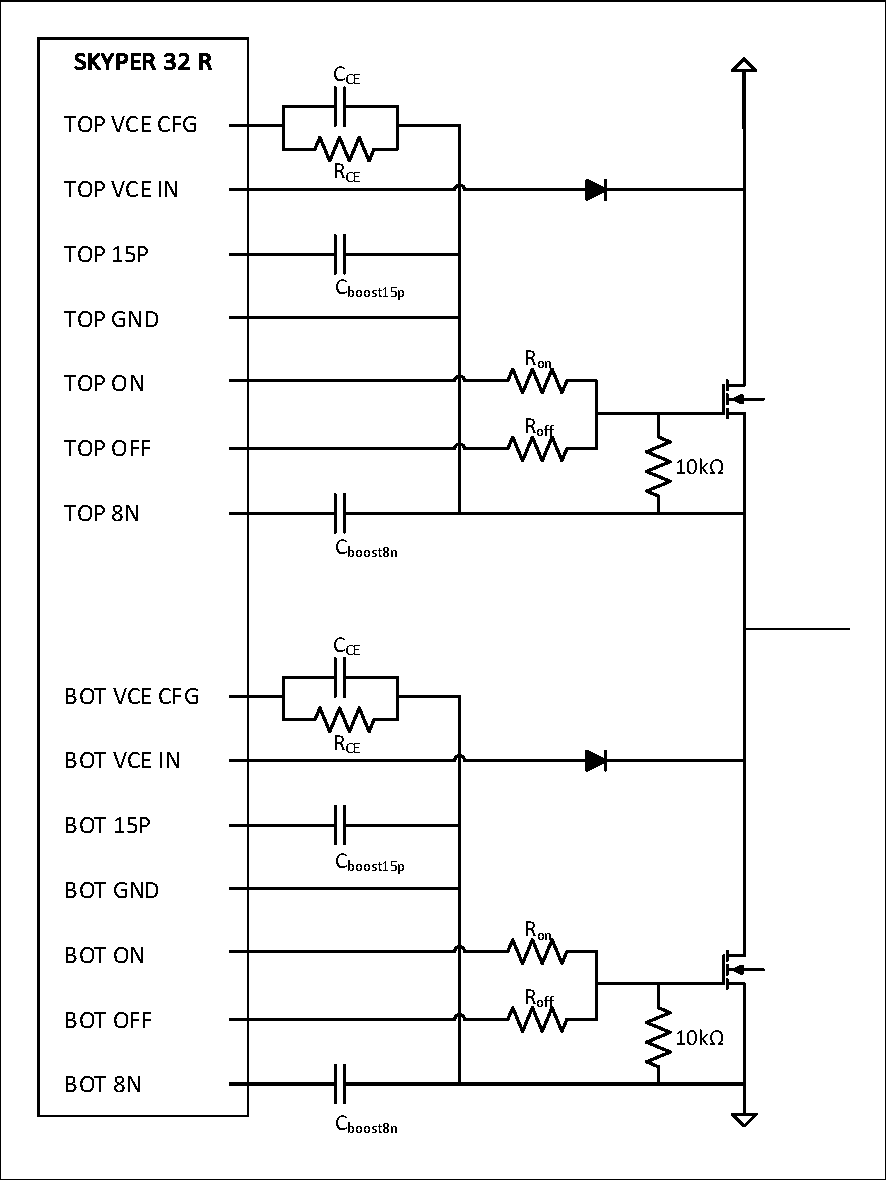
\includegraphics[width=0.5\textwidth]{figures/Skyperboard/Skyper32out.pdf}
    \caption{Circuit on the output of the SKYPER 32R}
	\label{fig:Skyper32out}
\end{figure}
\clearpage
As the SKYPER Board needs an input signal of 15V a circuit is needed to convert the 5V signal from the low power logic.
Therefore a small op-amp based comparator circuit was constructed.
It compares the input signal to 1.5 Volts, so every input above will result in a high output,
all inputs below as low.
This also allows to run it from a logic that only outputs 3V signals.

In Figure \ref{fig:Skyper32in} it can be seen how the input coming from the control logic with a 5V PWM signal and 15V power supply are connected to the amplification board.
On there the signal gets raised to 15V PWM and the board also includes the pull-up resistor to read out the open collector error out pin of the SKYPER 32R.
The board connects to the adaptor board that has the required capacitors and a pull up resistor for the error in.
The adaptor board is connected to all the inputs of the SKYPER 32R.

\begin{figure}[H]
   \centering
   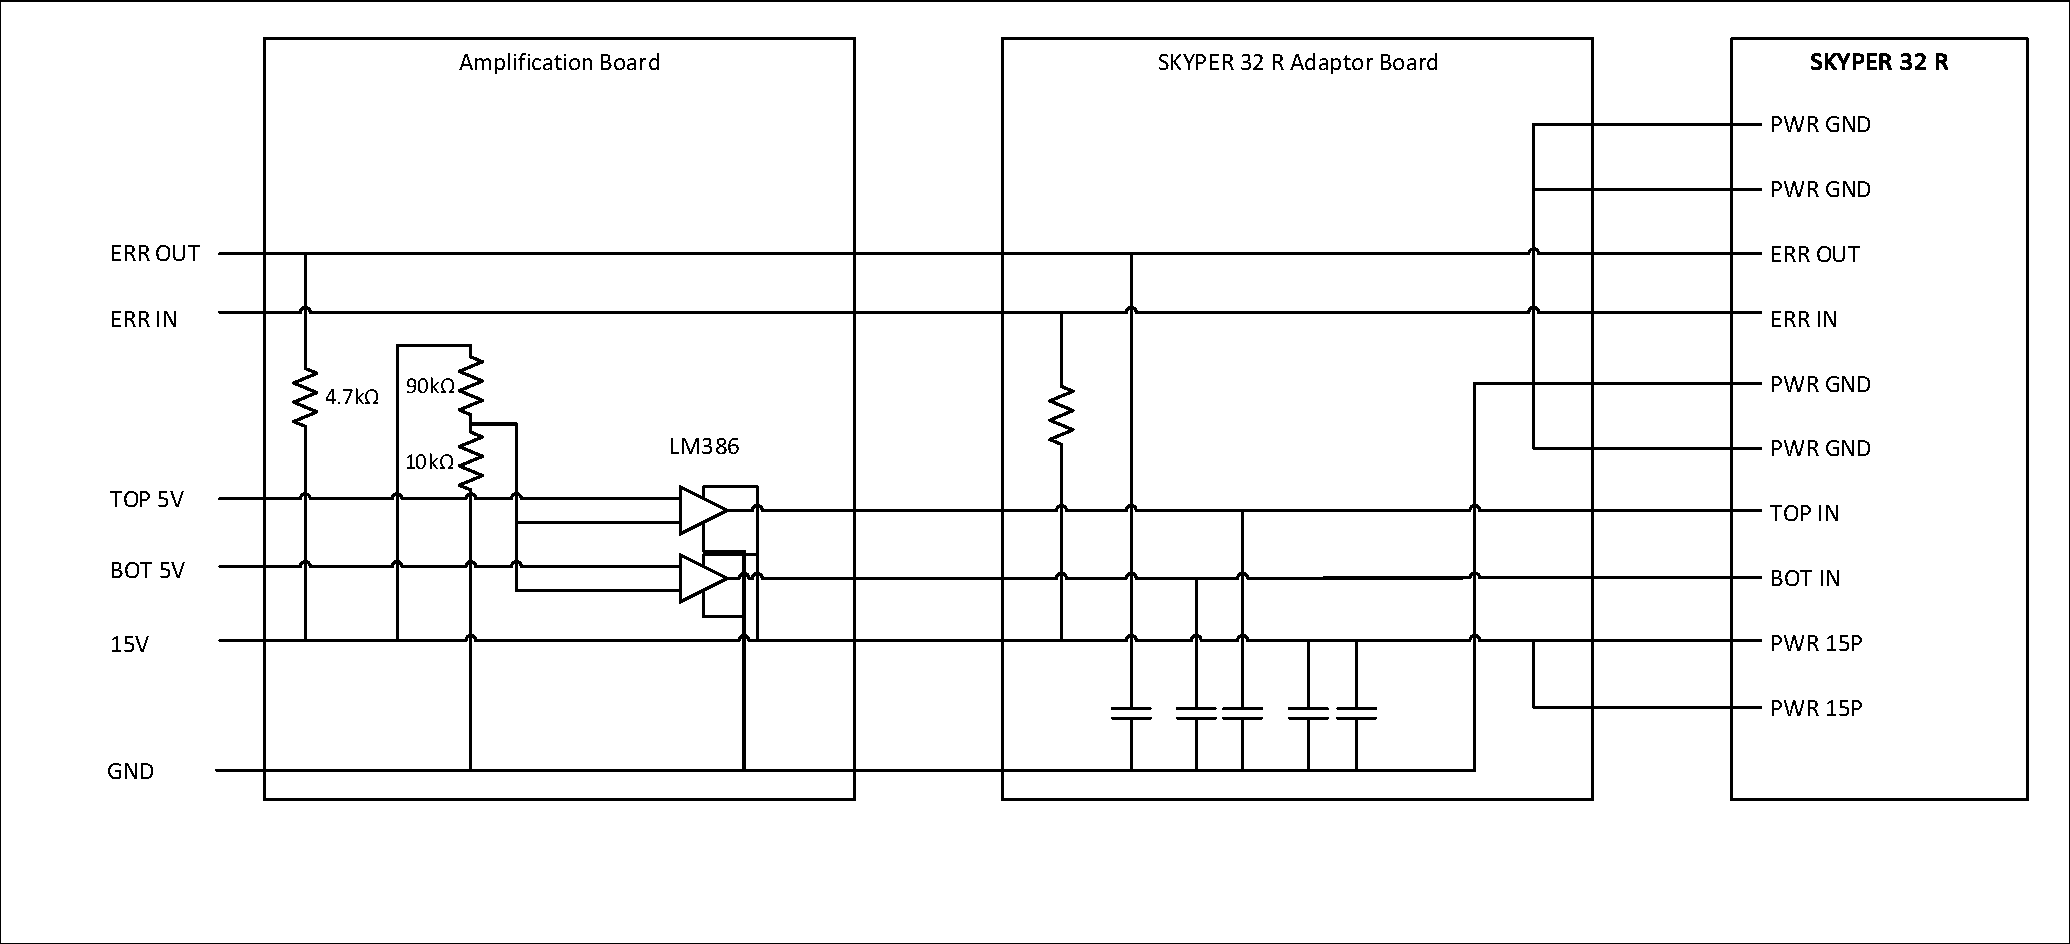
\includegraphics[width=\textwidth]{figures/Skyperboard/Skyper32in.pdf}
    \caption{Input boards for the SKYPER 32R}
	\label{fig:Skyper32in}
\end{figure}
The SKYPER board is intended for IGBT bridge circuits and therefore has a function which switches both devices off, if the input tries to turn them both on.\cite{SKYPER322:online} Therefore a second identical circuit and board will be used to drive each of the MOSFETs.

\clearpage
\section{PCB Design}\label{sec:PCB}

To be able to test the proposed topology,
a Printed Circuit Board (PCB) had to be made.
We started out designing a simple two stage layout,
and ended up manufacturing a three stage version.

\subsection{Two Stage PCB}
To get familiar with designing power electronics PCBs,
we started out designing a two stage version of the proposed topology.
Because we already had some familiarities with EAGLE from previous projects,
we used EAGLE for the first design attempts.
The finished design can be seen in Figure \ref{fig:2nxeagle}.

\begin{figure}[H]
	\begin{center}
	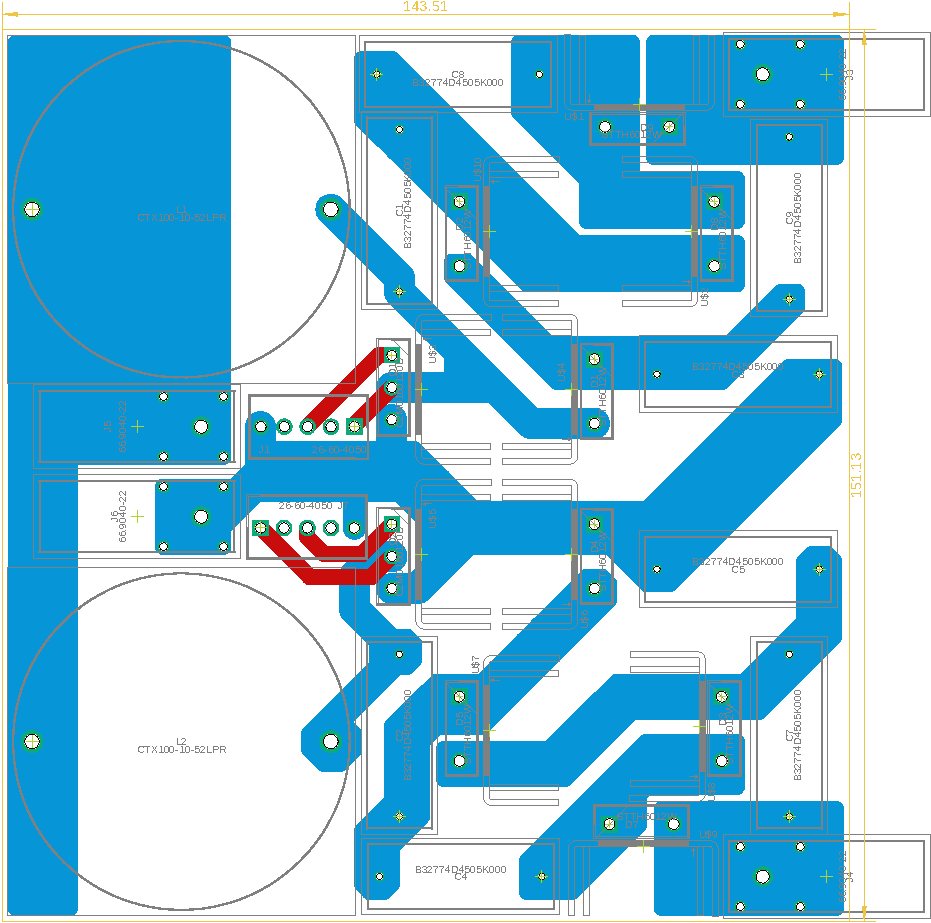
\includegraphics[width=0.6\textwidth]{figures/05cPCBdesign/2NX_interleaved_boost_converter_EAGLE_BY_DANIEL.pdf}
	\end{center}
	\caption{PCB Layout for a two stage 2NX Interleaved Boost Converter}
	\label{fig:2nxeagle}
\end{figure}

The red traces are logical signals,
located on the top layer of the PCB,
blue are power traces located on the bottom layer.
The power traces can be observed to be broader than the logic,
and were drawn as polygons,
to use the biggest available surface area.
The logical signals are designed to be as short as possible
and to be located as far from the power traces as possible,
to minimize interference.
\clearpage
Precautions were made in respect to the method of manufacturing,
because acute angles between two legs of a trace can lead to cracks in the trace when etching.
To prevent this from happening,
more copper was added in the areas in question to create obtuse angles.
A detailed view of this can be seen in Figure \ref{fig:2nxeagledetail}.
\begin{figure}[H]
	\begin{center}
	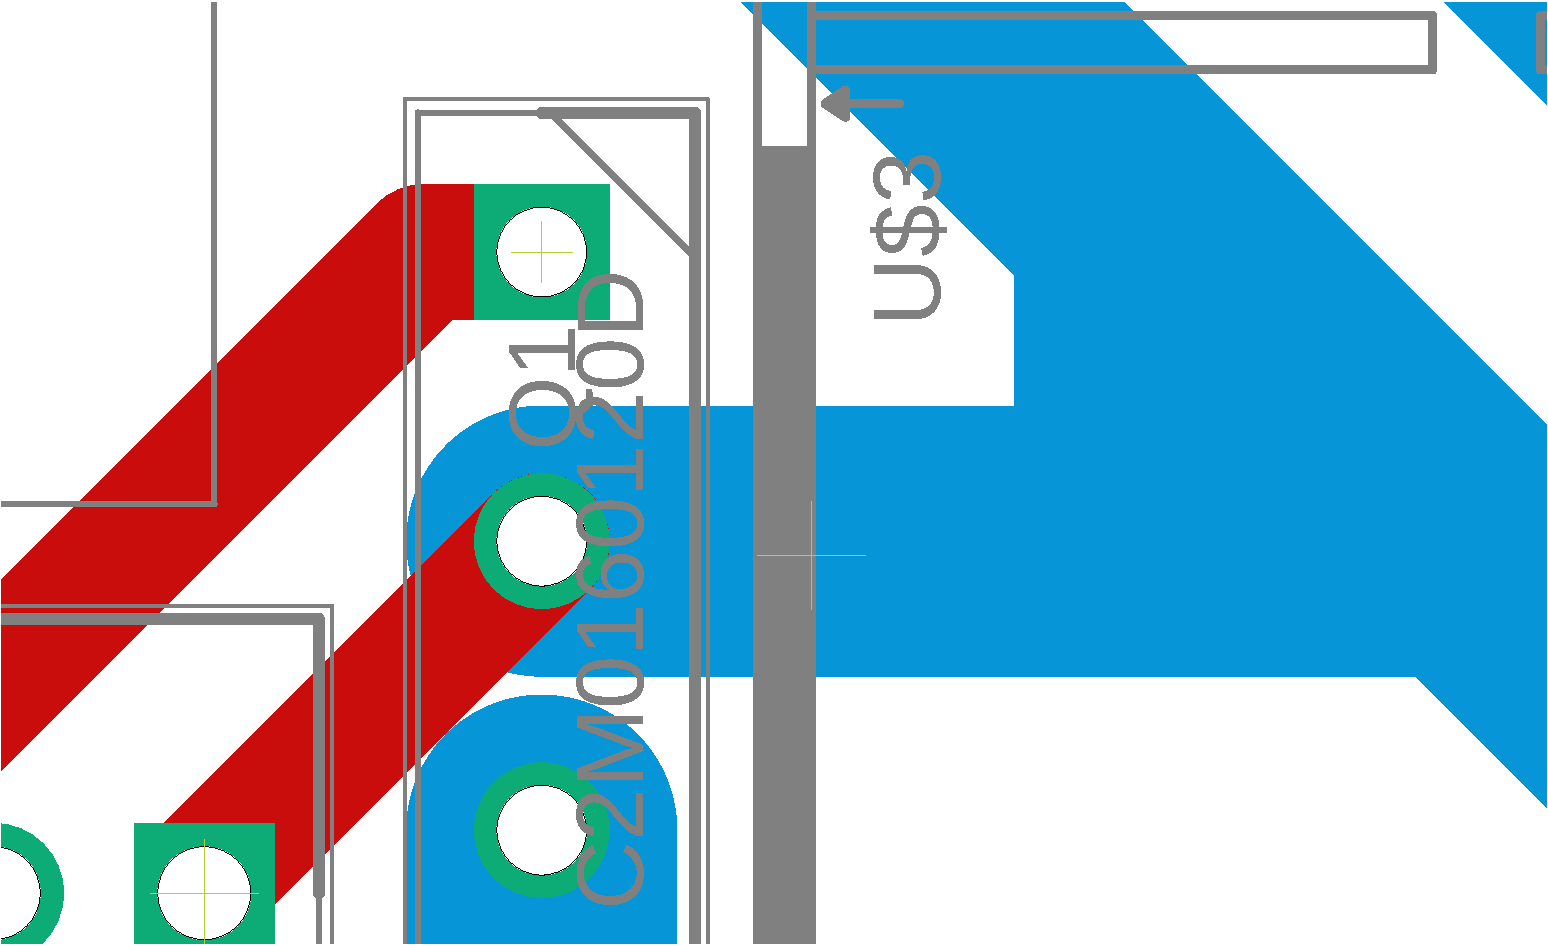
\includegraphics[width=0.6\textwidth]{figures/05cPCBdesign/2NX_interleaved_boost_converter_EAGLE_BY_DANIEL_DETAIL.pdf}
	\end{center}
	\caption{Detailed view of copper traces with obtuse angles}
	\label{fig:2nxeagledetail}
\end{figure}

\subsection{Three Stage PCB}\label{sub:3sPCB}
For the actual testing,
we decided on a three stage variant with our supervisor.
The PCB was again designed by us,
using feedback on the first design.
The power and logic traces are now on the same layer,
as it is not necessary to separate them as much.
The tracks generally are wider
and the spacing between is consistently kept at 2 mm.
The final PCB layout can be seen in Figure \ref{fig:multi2nxEAGLE}.

\begin{figure}[H]
	\begin{center}
	\includegraphics[height=1.0\textwidth,angle=270]{"figures/05cPCBdesign/FULL_3level_2NX_interleaved_boost_converter"}
	\end{center}
	\caption{PCB Layout for a multi stage 2NX Interleaved Boost Converter}
	\label{fig:multi2nxEAGLE}
\end{figure}
\vspace{+8mm}
The inductors and capacitors are different to the previous design,
because the new design reflects the components available to us.
To be able to connect the board to power and measurements,
banana plugs were suggested by our supervisor.

The inductor is not connected directly by soldering,
but through jumper cables.
This allows for easier access to the core and to fine tune the windings after testing.
This also makes measuring of voltage and current easier.

A detailed view showing the connectors for the top inductor can be seen in Figure \ref{fig:multi2nxDetail}.\\
The banana plugs for connecting the inductor are shown in red.

\begin{figure}[H]
	\begin{center}
	\includegraphics[width=0.5\textwidth]{"figures/05cPCBdesign/DETAiL_3level_2NX_interleaved_boost_converter"}
	\end{center}
	\caption{Detailed view of the inductor connection}
	\label{fig:multi2nxDetail}
\end{figure}

%
%\section{Static Modelling}\label{sec:statmod}
%
%\subsubsection{Single Pump Model}
%
%\begin{equation}
%	H = \bar{a_{2}} \cdot Q^2 + \bar{a_{1}} \cdot Q + \bar{a_{0}}
%	\label{eq:pumpHeadModel}
%\end{equation}
%\begin{equation}
%	P = \bar{b_{3}} \cdot Q^3 + \bar{b_{2}} \cdot Q^2 + \bar{b_{1}} \cdot Q + \bar{b_{0}}
%	\label{eq:pumpPowerModel}
%\end{equation}
%
%\begin{align*}
%	\left(\frac{\omega_1}{\omega_2}\right)^1 = \frac{Q_1}{Q_2} && 
%	\left(\frac{\omega_1}{\omega_2}\right)^2 = \frac{H_1}{H_2} &&
%	\left(\frac{\omega_1}{\omega_2}\right)^3 = \frac{P_1}{P_2}		
%\end{align*}\cite{Volk2014}.
%
%\begin{equation}
%	H(\omega) = a_0 \cdot \omega^2 + a_1 \cdot \omega \cdot Q(\omega) + a_2 \cdot Q(\omega)^2
%	\label{eq:pumpHeadModel2}
%\end{equation}
%\begin{equation}
%	P(\omega) = b_0 \cdot \omega^3 + b_1 \cdot \omega^2 \cdot Q(\omega) + b_2 \cdot \omega \cdot Q(\omega)^2 + b_3 \cdot Q(\omega)^3
%	\label{eq:pumpPowerModel2}
%\end{equation}
%
%\begin{align*}
%	a_0 = \frac{\bar{a_0}}{\bar{\omega_0^2}} && a_1 = \frac{\bar{a_1}}{\bar{\omega_0}} && a_2 = \bar{a_2} \\
%	b_0 = \frac{\bar{b_0}}{\bar{\omega_0^3}} && b_1 = \frac{\bar{b_1}}{\bar{\omega_0^2}} && b_2 = \frac{\bar{b_2}}{\omega_0} && b_3 = \bar{b_3}
%\end{align*}
%\cite{Yang2010}
%
%%\begin{figure}[ht]
%%	\centering
%%	\includegraphics[width=1\textwidth]{figures/05mathematicalModelling/flowVsPowerRun34.eps}
%%	\caption{Data Points for Flow vs. Power Consumption}
%%	\label{fig:flowVsPowerConsumption}
%%\end{figure}
%
%\begin{align*}
%	a_0 = -0.03044 && a_1 = 0.07635  && a_2 = 1.688  \\
%	b_0 = -0.2825 && b_1 = -0.7147 && b_2 = 54.39 && b_3 = 163.7 \\
%\end{align*}
%
%\section{Dynamic Modelling}\label{sec:dynMod}
%
%\begin{equation}
%	\frac{Y(s)}{U(s)} = \frac{A \cdot e^{-st_d}}{\tau \cdot s + 1}
%	\label{eq:plantTransferFunction}
%\end{equation}
%
%\begin{itemize}
%	\item A = final value the step response settles at
%	\item $t_{d}$ = time delay
%	\item $\tau$ = time it takes from 0.1 of final value to 0.9 final value
%\end{itemize}

%
%
%
\chapter{Testing}\label{ch:testing}

\section{Setup}
All the components listed in Section \ref{ch:compSpec} were mounted on the PCB (can be seen on Fig. \ref{fig:SETUP}) and all the driver circuit were built to be connected to the full setup.
Standard lab power supplies were used to deliver all the inputs needed to the op-amps, SKYPER boards and the input voltage of the circuit itself. 
The maximum output current of the power supply is 3.2A.
For the load a rheostat was used, so that the load can be adjusted to the capabilities of the power supply and the resistance it was set to for the tests was 2.5k$\Omega$ . 

\begin{figure}[H]
	\begin{center}
   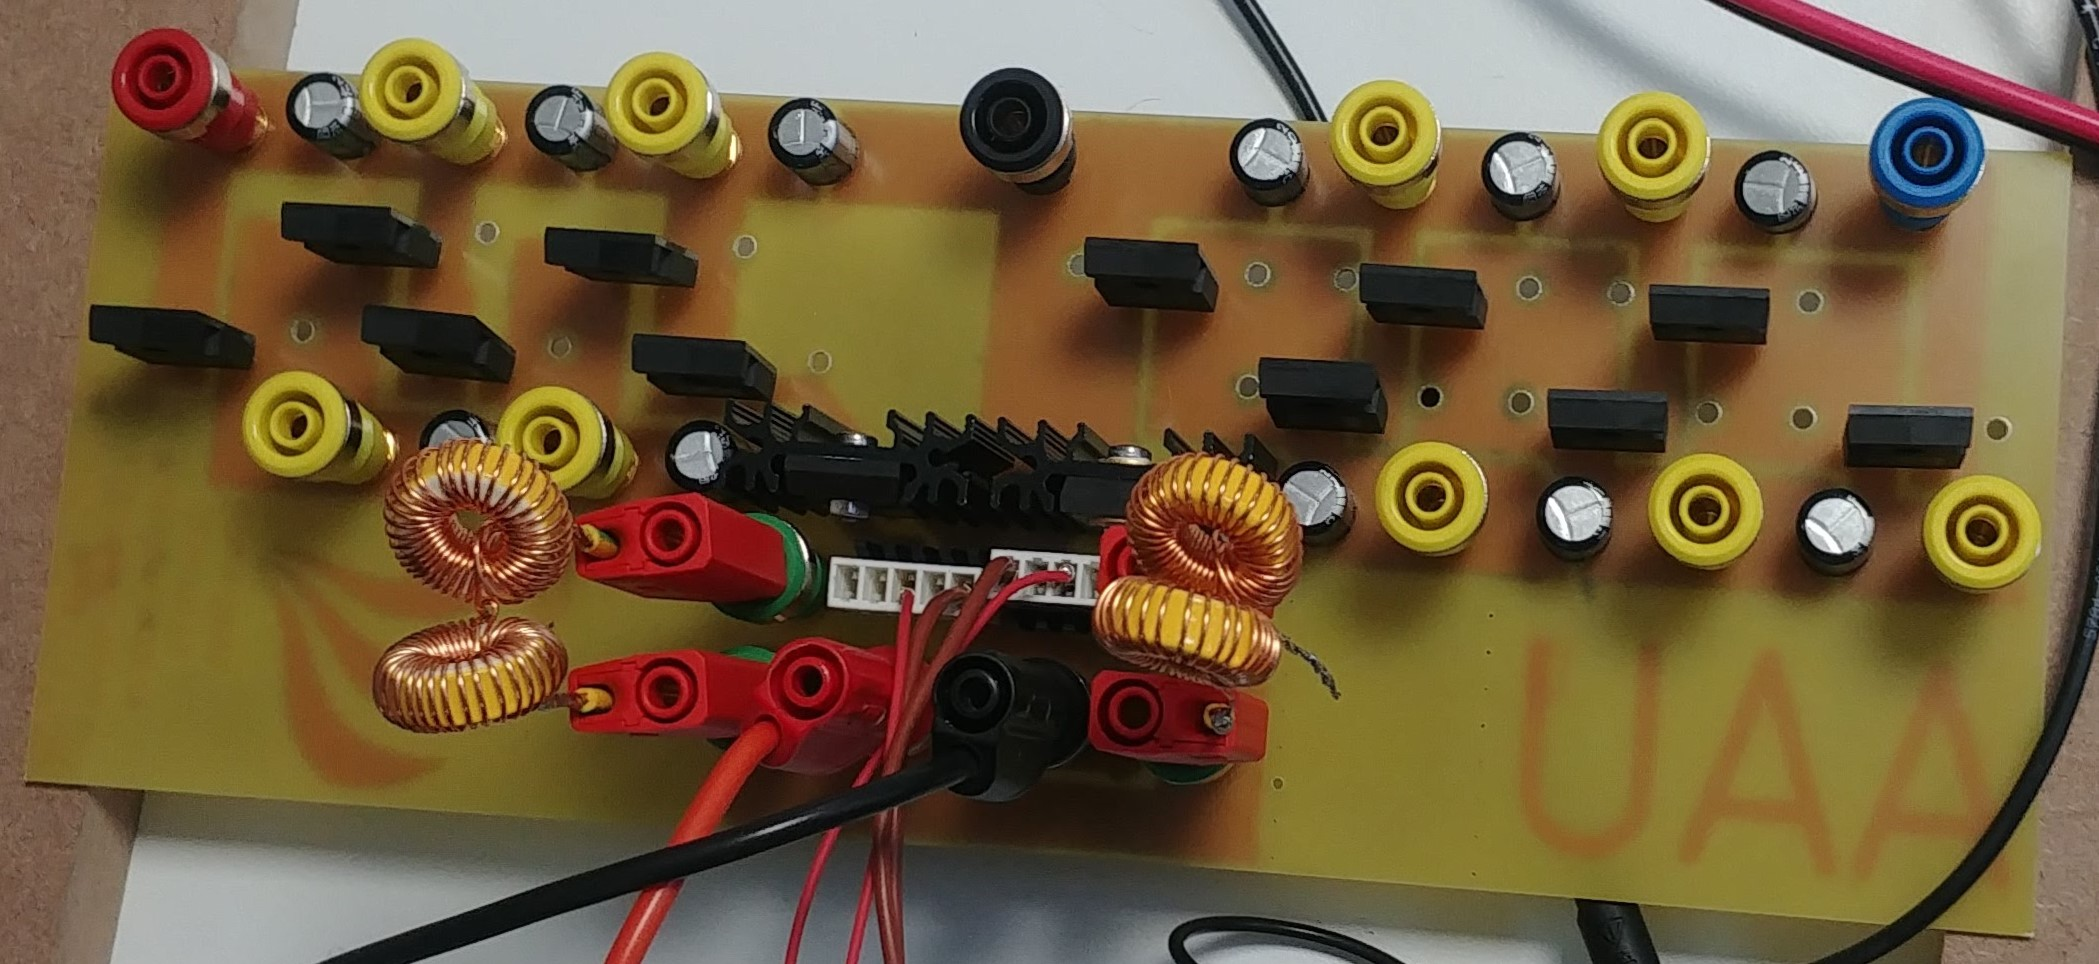
\includegraphics[width=0.8\textwidth]{figures/06Testing/setup.jpg}
	\end{center}
	\vspace{-4mm}
	\caption{PCB with all the components mounted}
	\label{fig:SETUP}
\end{figure}

To generate the PWM input, two wave generators were used, due to the easy synchronisation. The tools used for measurements were ... Oscilloscopes and ... multimeters, all available for us in the AAU Esbjerg laboratories.
All the data presented in the next section has been captured in these devices, results are limited to their accuracy.
\todo {names of scopes} 
\clearpage
\vspace{-6mm}
\section{Results}

After the setup was complete the first test ran, to test the overall output voltage of the topology within the range of possible duty cycles. The purpose of this tests is too see if the expected gain is matched and what part of the differences are expected and what the unexpected ones can be justified by. 
\vspace{-4mm}

\begin{figure}[H]
	\begin{center}
   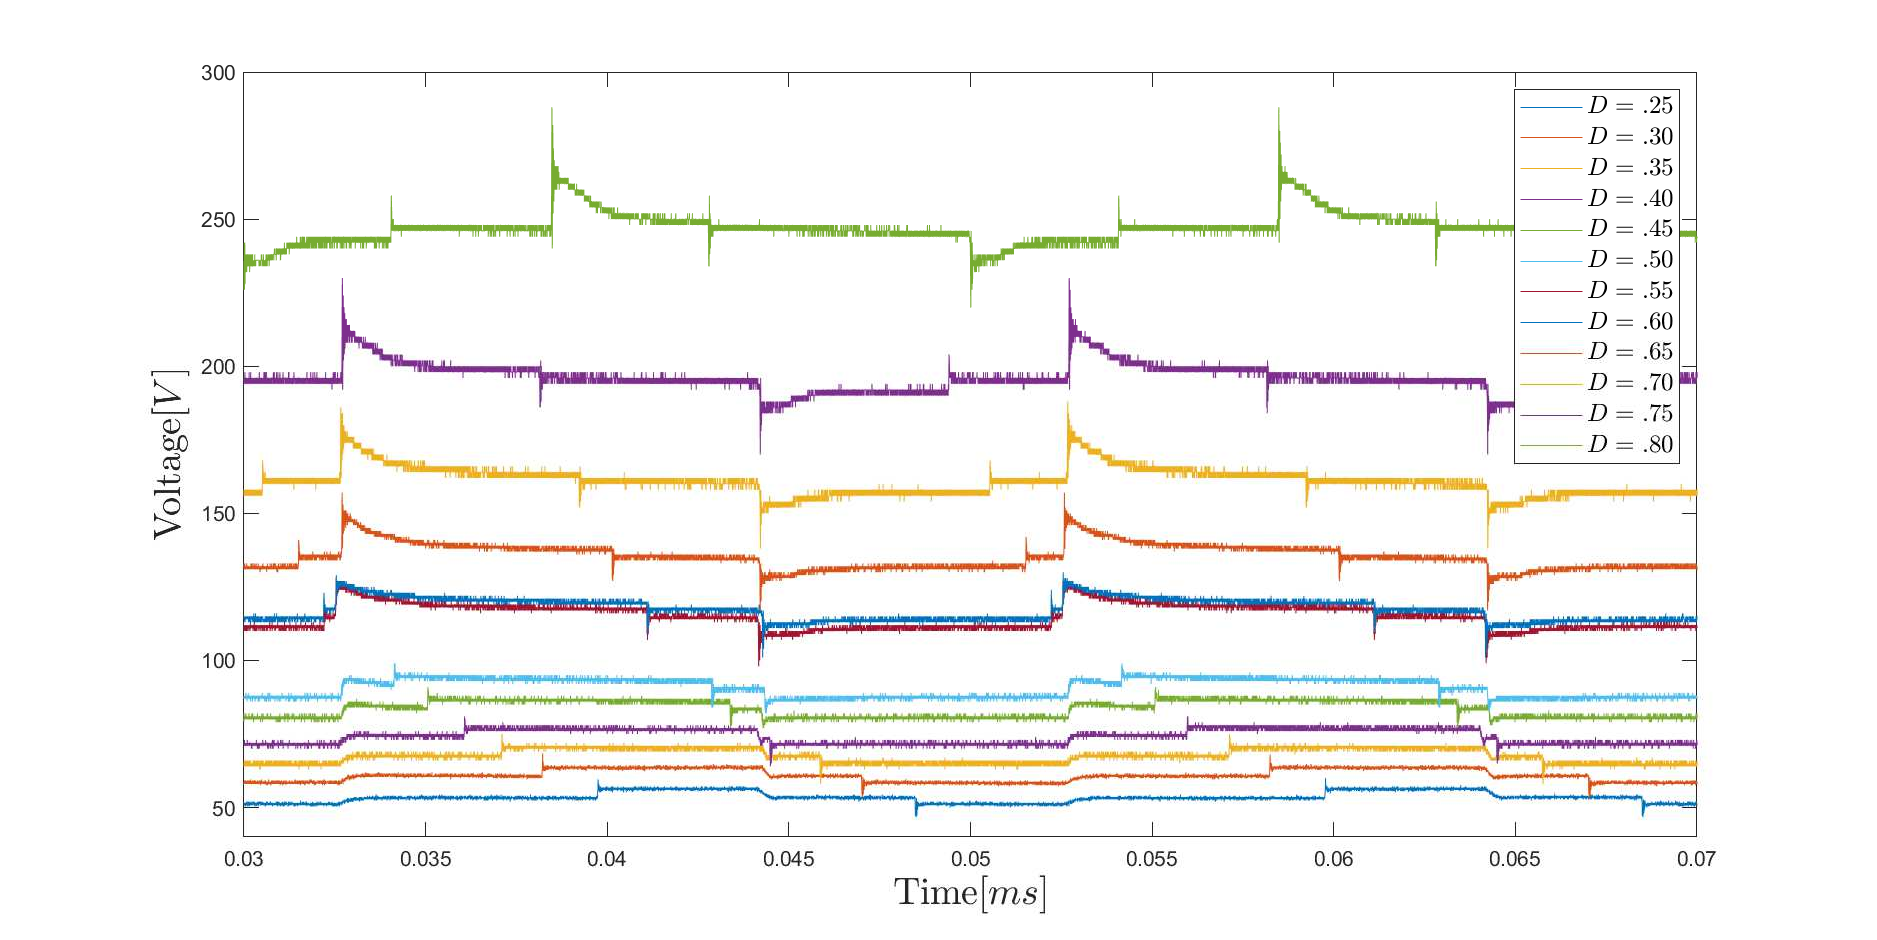
\includegraphics[width=\textwidth]{figures/06Testing/Vripple10Vin.pdf}
	\end{center}
	\vspace{-8mm}
	\caption{$V_o$ at duty cycles between 0.25 and 0.8}
	\label{fig:V_OUT_ALL}
\end{figure}
\vspace{-4mm}
All the output voltage waves can be seen on Fig. \ref{fig:V_OUT_ALL}. To put those values, they need to be compared to the expected values from the expressions we've already derived. All of the calculated and measured values can be seen in the Table \ref{tab:V_OUT_ALL}.
\vspace{-2mm}

\begin{table}[H]
\begin{center}
\caption {Calculated and Measured output voltages} \label{tab:V_OUT_ALL} 
\vspace{-1mm}
\begin{tabular}{|l|l|l|l|}
\cline{1-4}
Duty cycle & Calculated $V_o$ & Measured $V_o$& Difference \\ \cline{1-4}
0.25&	63.9V & 52.6V & 11.3V \\ \cline{1-4}
0.30&	70.0V & 59.7V & 10.3V \\ \cline{1-4}
0.35&	75.9V & 66.1V & 9.8V \\ \cline{1-4}
0.40&	82.9V & 71.8V & 11.1V \\ \cline{1-4}
0.45&	92.2V & 76.4V & 15.7V \\ \cline{1-4}
0.50&	102.4V & 83.3V & 19.1V \\ \cline{1-4}
0.55&	114.9V & 93.1V & 21.8V \\ \cline{1-4}
0.60&	125.0V & 106.8V & 18.2V\\ \cline{1-4}
0.65&	144.3V & 123.9V & 20.4V \\ \cline{1-4}
0.70&	162.4V & 147.0V & 15.4V\\ \cline{1-4}
0.75&	194.2V & 182.5V & 11.7V \\ \cline{1-4}
0.80&	245.8V & 221.0V & 24.8V\\ \cline{1-4}
&	 & Average loss:  & 15.8V \\ \cline{1-4}
\end{tabular}
\end{center}
\end{table}

The results show variable difference in favour of the calculated values. That is completely expected as all of the components apart from the diode and MOSFET were assumed ideal. Internal resistance and power consumption of all components can justify some of the losses. What is less expected is that there is no clear pattern in the decreases, which can be accounted to imperfect measurement or overall inconsistency in the tests and/or equipment. 

To validate our simulation results,
we tested the hardware in depth at a duty ratio $D = 0.6$.
This is the standard we used throughout all simulations described in Chapter \ref{ch:dev}.
We took all measurements possible with our board layout,
which mostly allowed for voltage measurements between components.
The only place where we could measure the current was at the inductors.

Figure \ref{fig:bottopcharge} shows a comparison of the charging components.

\begin{figure}[H]%
    \centering
    \subfloat[Bottom Capacitor Voltages]
    {{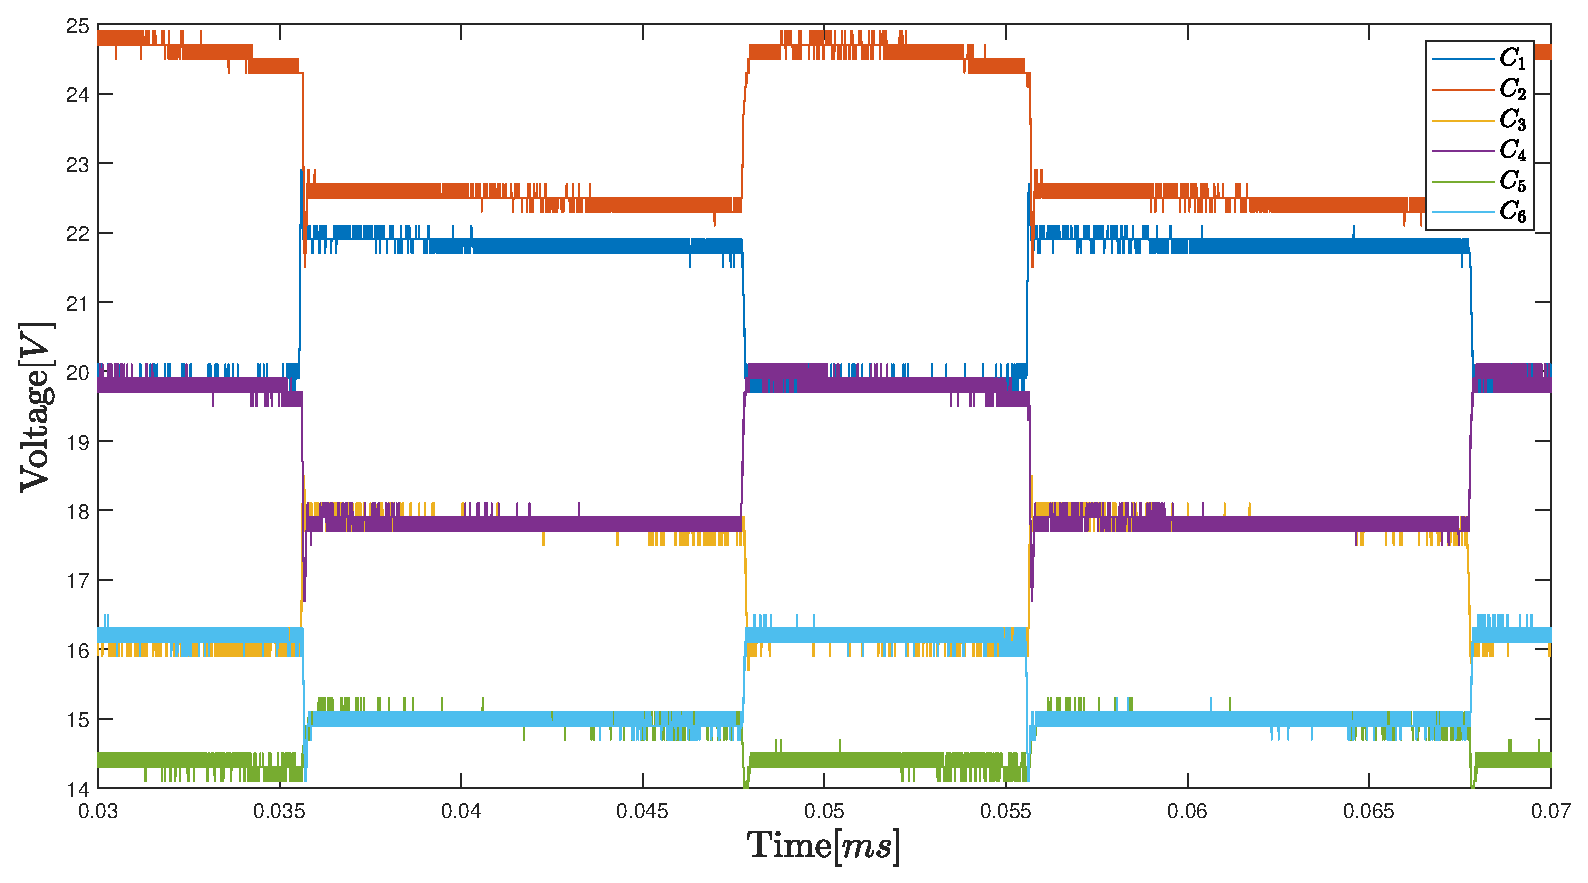
\includegraphics[width=0.5\textwidth]{figures/06Testing/botcap60per.eps} \label{fig:botcap60per}}}%
    \subfloat[Top Capacitor Voltages]
    {{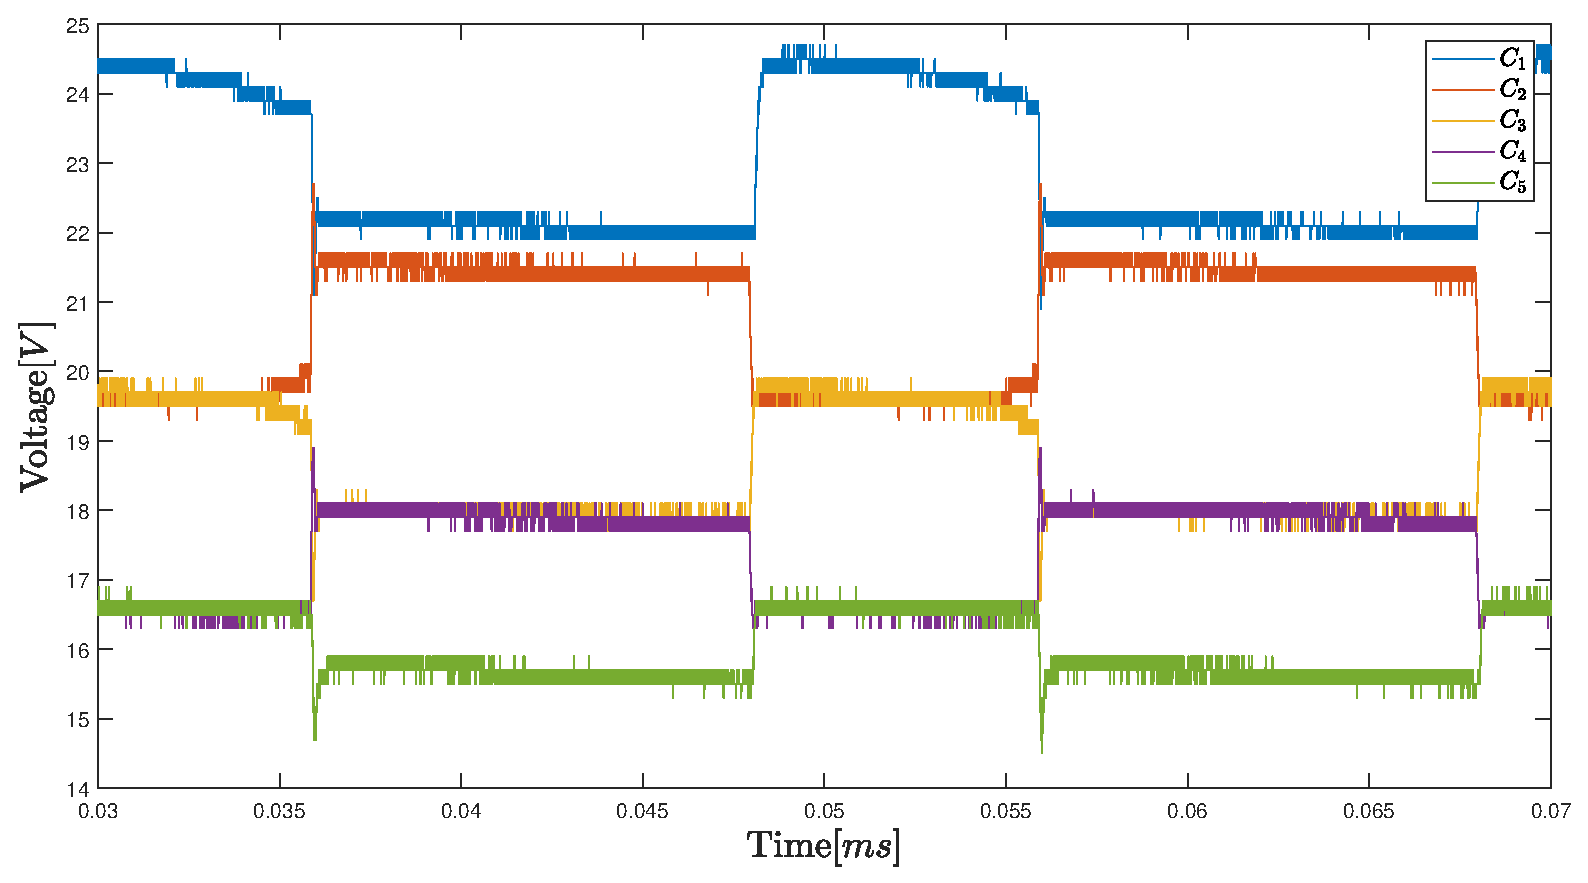
\includegraphics[width=0.5\textwidth]{figures/06Testing/topcap60per.eps} \label{fig:topcap60per}}}%  
   \qquad
    \subfloat[Bottom Inductor Current/Voltage]
    {{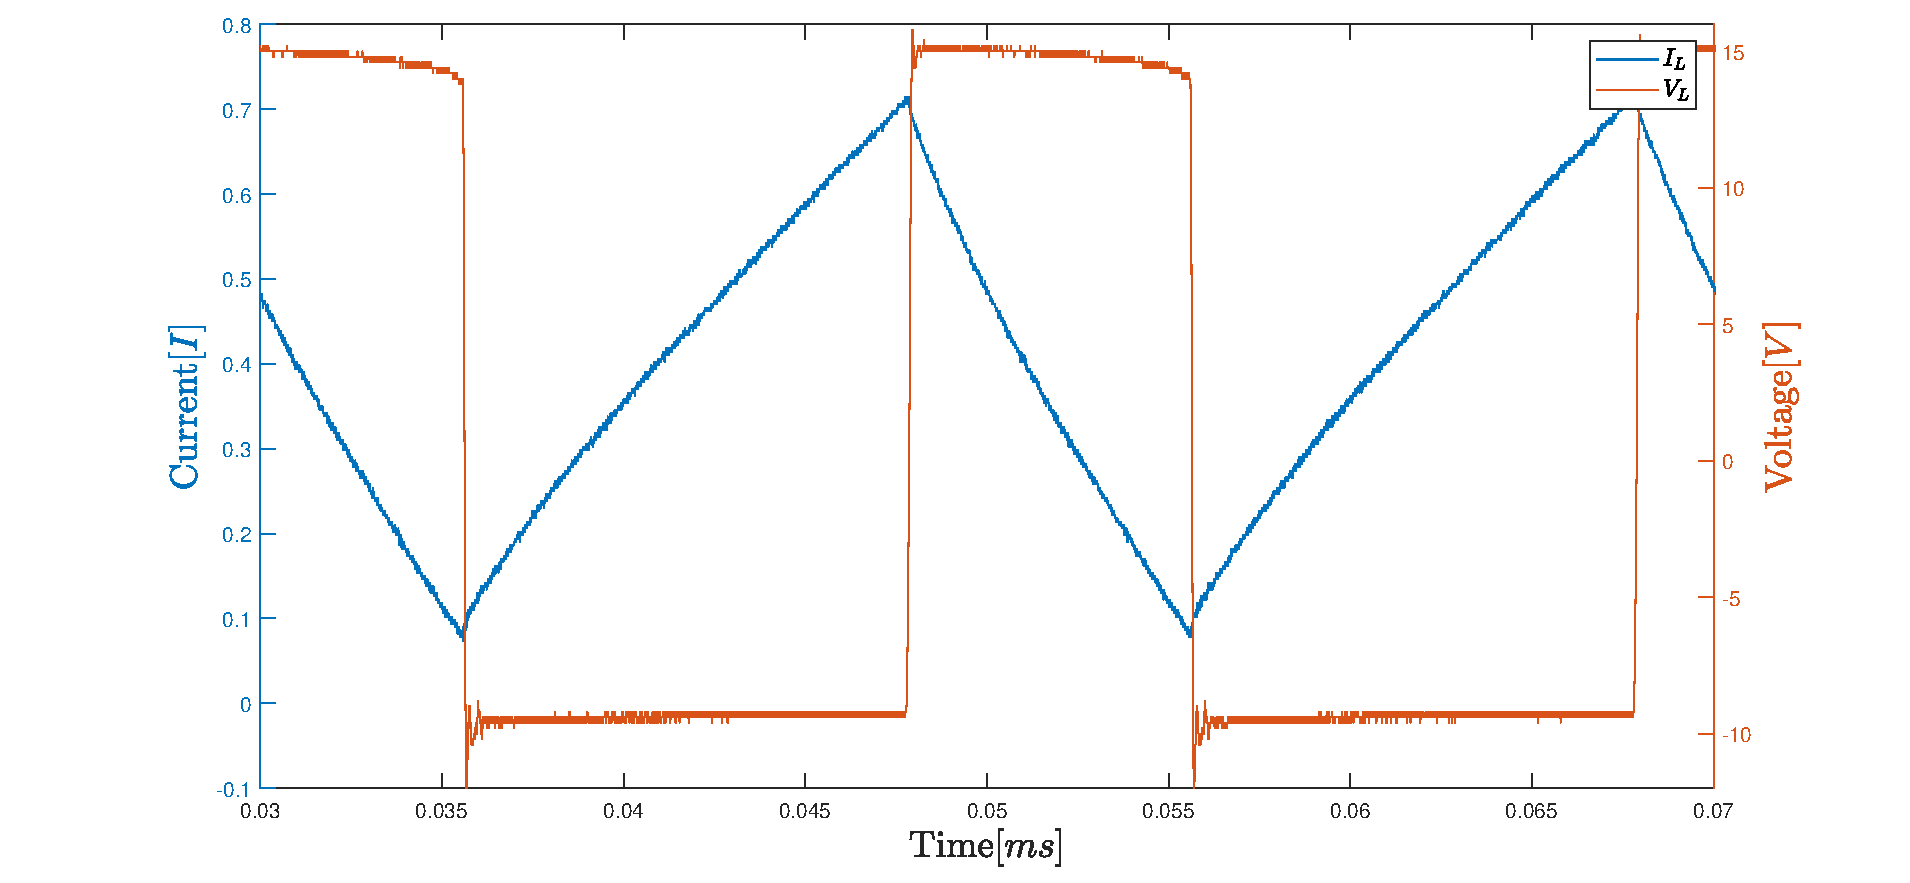
\includegraphics[width=0.5\textwidth]{figures/06Testing/botind60per.eps} \label{fig:botind60per}}}%
    \subfloat[Top Inductor Current/Voltage]
    {{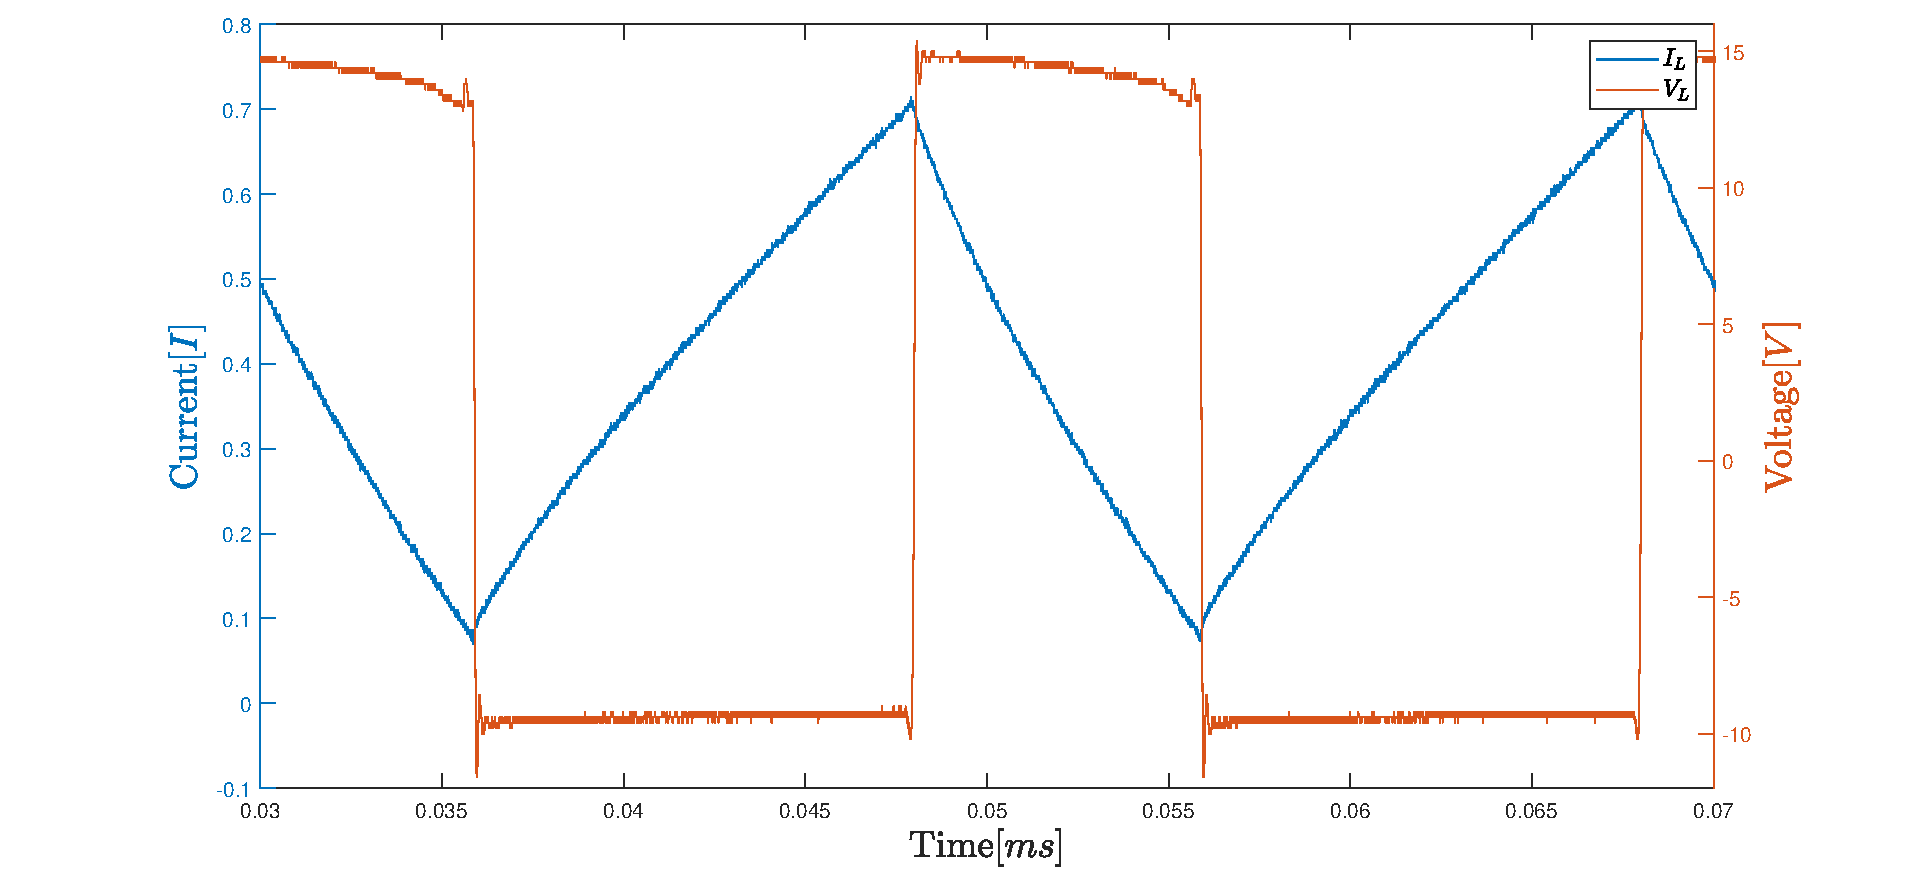
\includegraphics[width=0.5\textwidth]{figures/06Testing/topind60per.eps} \label{fig:topind60per}}}%  
    \caption{Bottom/Top Comparison of Charging Components}%
     \label{fig:bottopcharge}%
\end{figure}
\todo{put figures in appendix}

To be noted is that the bottom (\ref{fig:botcap60per}) is an inverting NxBC,
while the top is non inverting.
Because of that the naming of the capacitors varies slightly.
For simplicity,
we will from now on only talk about the top measurements (visible on the right).

It can be observed that the capacitor voltage $V_{C_1}$ is higher than the other voltages,
as expected in Chapter \ref{ch:dev}.
Also the voltage across this capacitor fits perfectly to the simulations,
with a mean of $23.5 V$.
The subsequent capacitors all have a falling voltage,
compared to the previous,
which suggests that our drop calculation is correct.
The amount of drop between the stages is higher than in the simulations,
which we expected,
because we used ideal components to simulate capacitors and inductors.

The repetitive charging and discharging heats both inductors and capacitors up,
which was not included in the simulations.
Also the internal resistance was neglected in the simulations.
The drops between the stages,
suggests a limited amount of stages to be beneficial.
This is a commonly known problem with the Cockcroft-Walton Multiplier.


Investigating the inductors current and voltage (\ref{fig:botind60per} \& \ref{fig:topind60per}),
we can observe that the converter is in continuous conduction mode (CCM) at $D = 0.6$.
There is even the option to go to a lower $D$,
as the current doesn't reach $0 A$.
The current is very low in total,
because $R_L$ was chosen very big.

The voltage across the inductors can be observed to have a range from $-10 V$ to $15V$.
The negative offset is observed because the negative measuring point is directly connected to $V_{IN} +$
The total range of the inductor voltage is $25V$, which is also the highest $C_{1}$ charges up to.





\begin{figure}[H]%
    \centering
    \subfloat[Bottom Diode Voltages]
    {{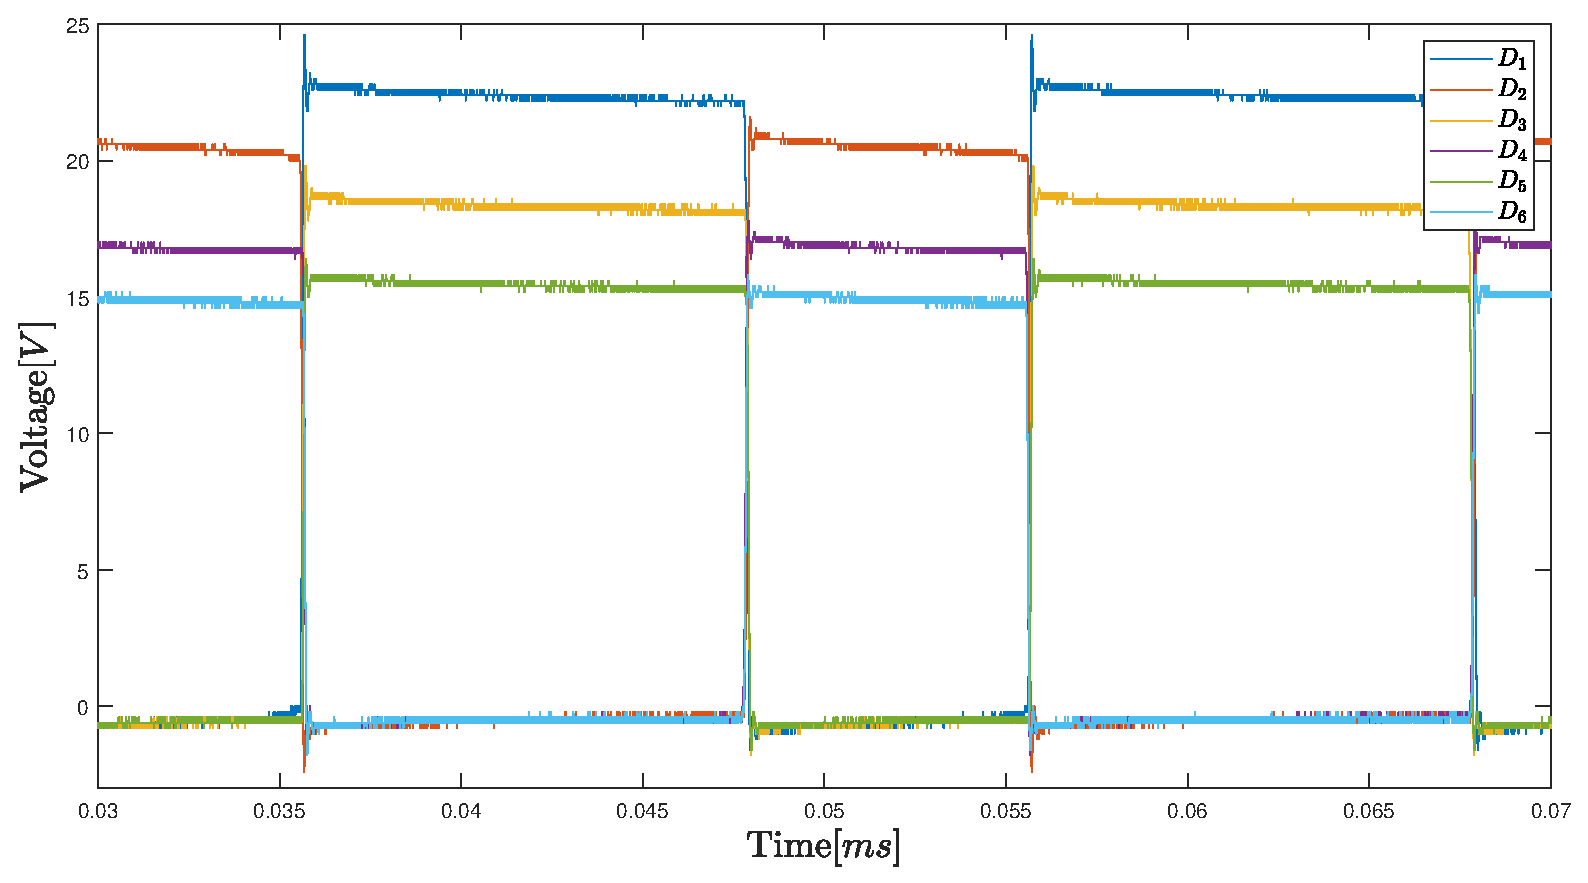
\includegraphics[width=0.5\textwidth]{figures/06Testing/botdio60per.eps} \label{fig:botdio60per}}}%
    \subfloat[Top Diode Voltages]
    {{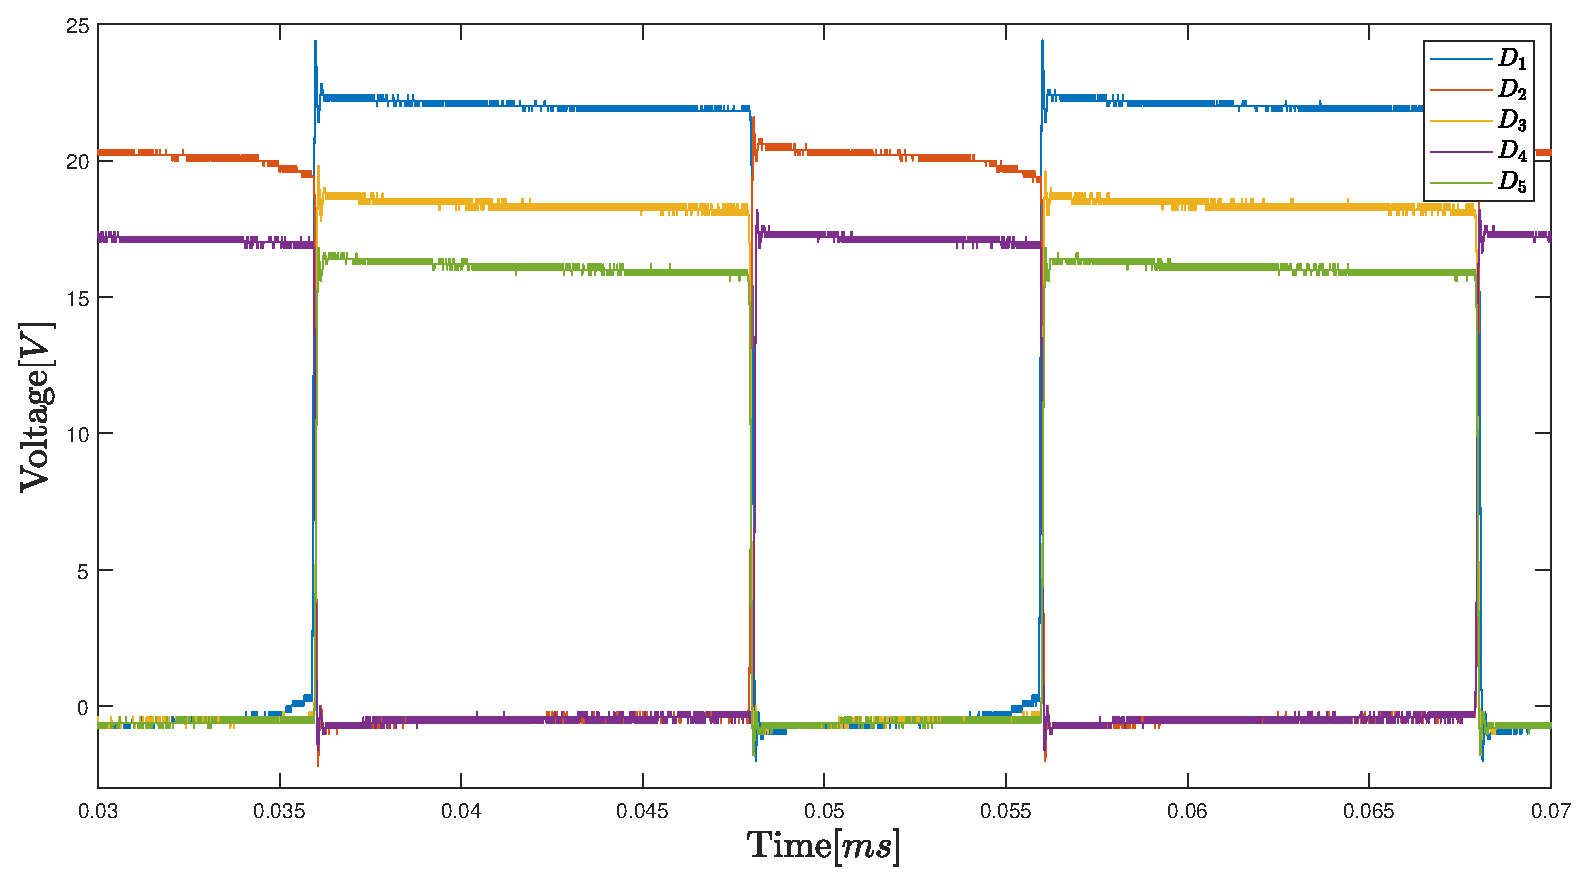
\includegraphics[width=0.5\textwidth]{figures/06Testing/topdio60per.eps} \label{fig:topcap60per}}}%  
   \qquad
    \subfloat[Bottom MOSFET Current/Voltage]
    {{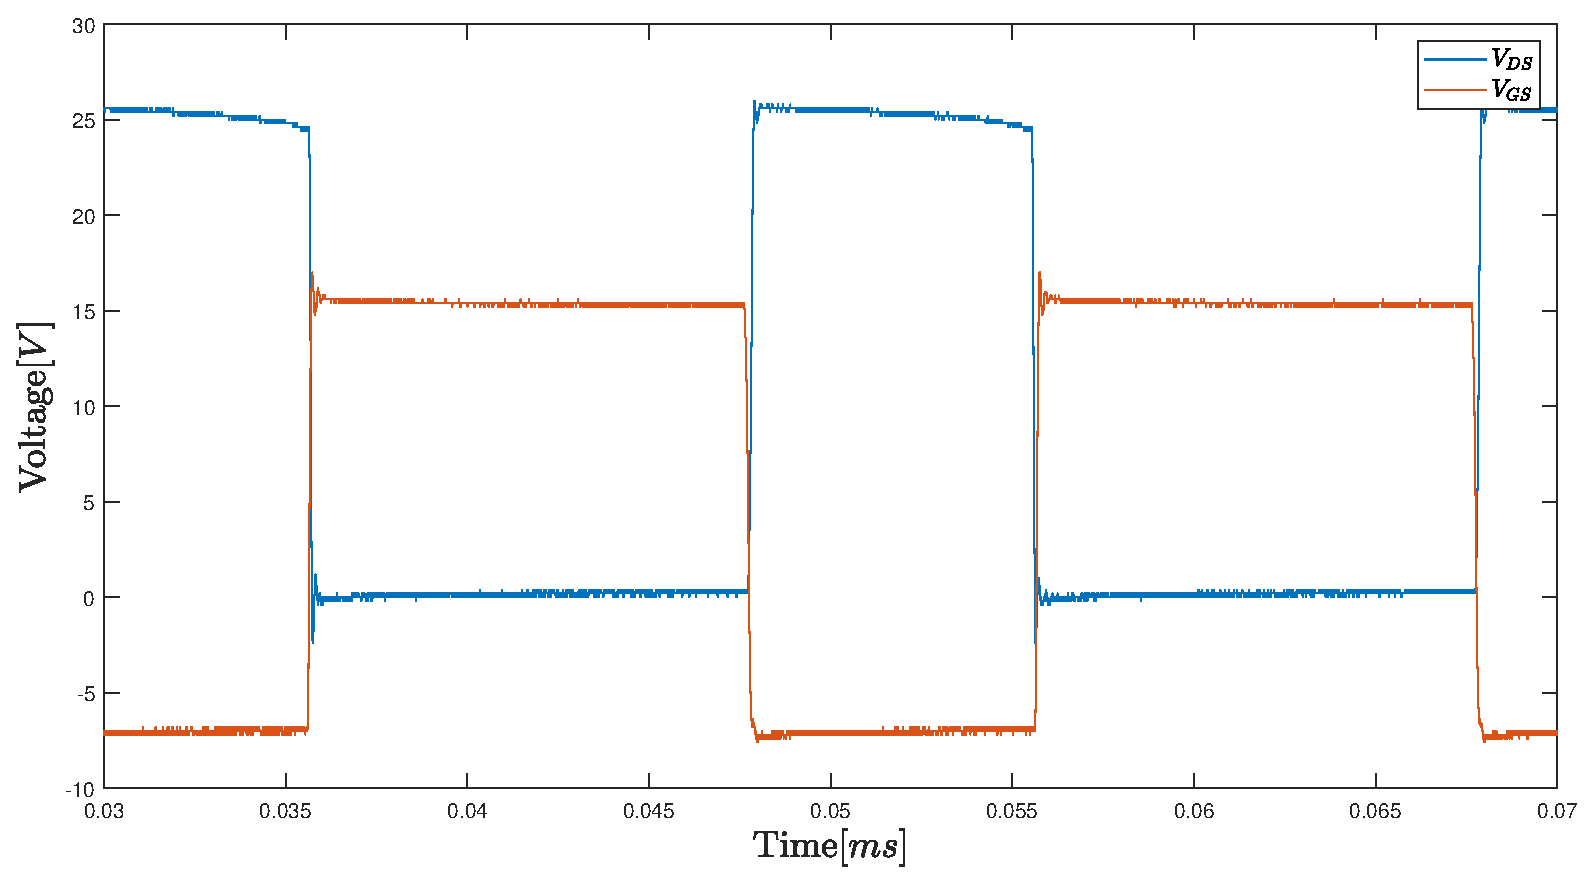
\includegraphics[width=0.5\textwidth]{figures/06Testing/botswi60per.eps} \label{fig:botind60per}}}%
    \subfloat[Top MOSFET Current/Voltage]
    {{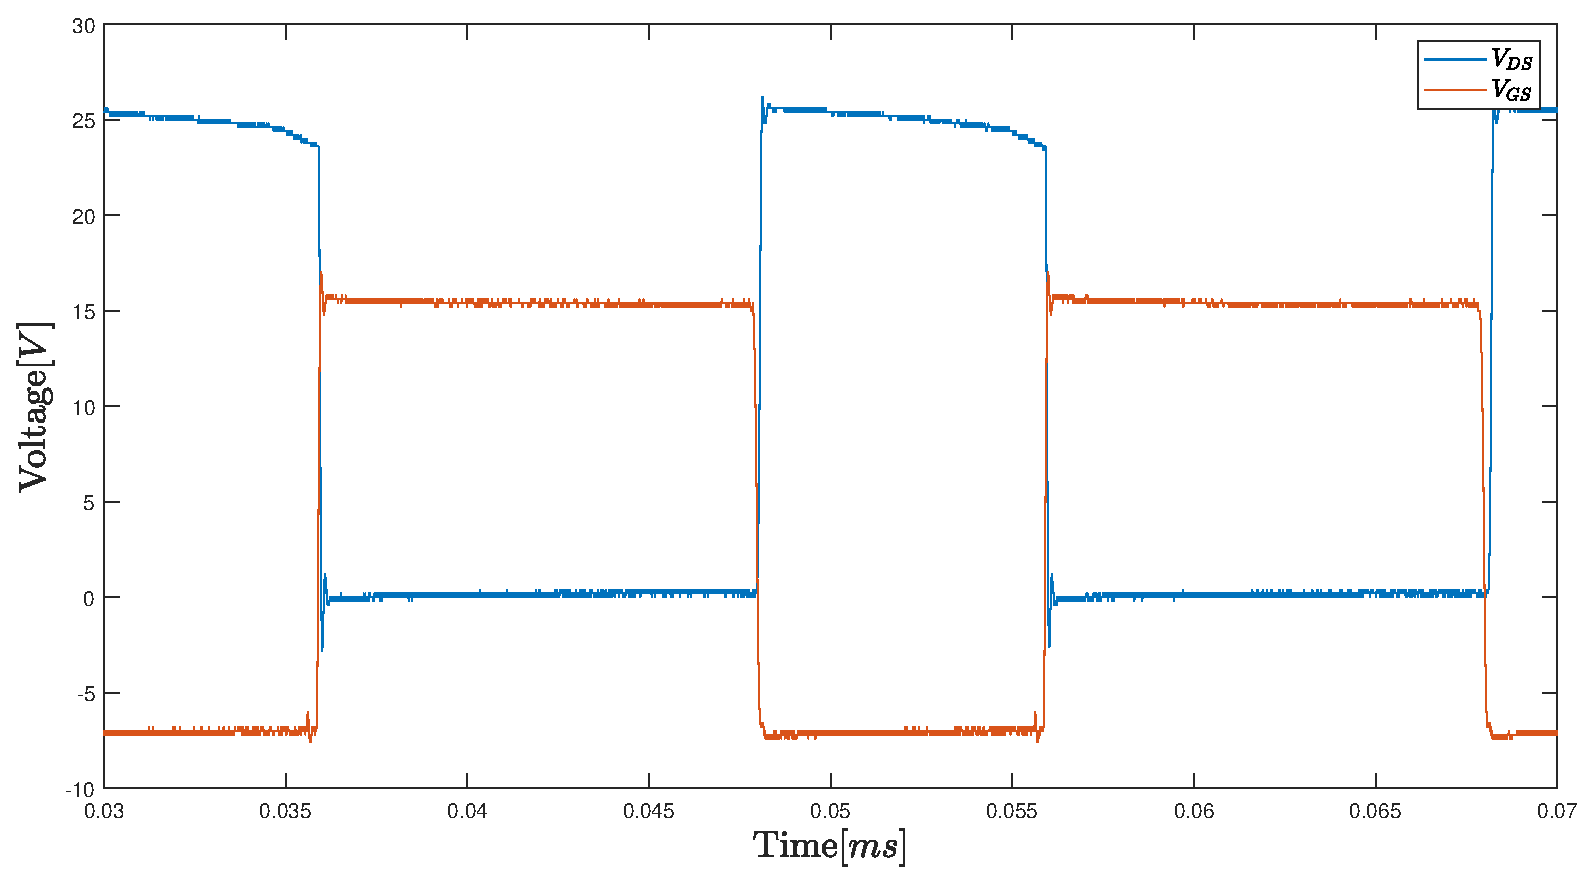
\includegraphics[width=0.5\textwidth]{figures/06Testing/topswi60per.eps} \label{fig:topind60per}}}%  
    \caption{Bottom/Top Comparison of Switching Components}%
     \label{fig:bottopswitch}%
\end{figure}
\todo{put figures in appendix}

The plot on Figure \ref{fig:bottopswitch} show the voltages across the diodes and across the terminals of the MOSFET.
The voltage levels over the diode confirm the statement already made about the capacitors - the voltage decreases over the higher levels of the circuit.
Another significant observation is that the negative voltage level is relatively consistent over the circuit, which improves the validity of the calculations in Section. \ref{ch:DROPS}.

The first conclusion we can draw from the MOSFET graphs is that the levels of $V{GS}$ confirm our switching circuit. 
The fact that the level are equal to the ones coming from the SKYPER board and the duty cycle is as expected proves that. 
The second major observation is that the stress over the switch $V{DS}$ during OFF state is equal to that of a CBC. 
This means that the requirements for a MOSFET for this topology are the same as the ones for a CBC, while the gain is higher.

To measure the efficiency of the converter the power on the input and output was measured.
This was done by taking the current from the source at a constant voltage and the current through the load, which size was known. So the powers and efficiency can be calculated.

% Pin = Vin*Iin Pout = I^2*R
\begin{equation}
	P_{in}= V_{in} \times I_{in}
	\label{eq:EfficiencyPin}
\end{equation}

\begin{equation}
	P_{out}= I_{out}^2 \times R_{load}
	\label{eq:EfficiencyPout}
\end{equation}

\begin{equation}
	\eta = (\frac{P_{out}}{P_{in}})
	\label{eq:Efficiency}
\end{equation}


The measured efficiency for different duty ratios can be found in the table below.

\begin{table}[H]
\begin{center}
\caption {Efficiency of the converter} \label{tab:Efficiencyandpowers} 
\vspace{-1mm}
\begin{tabular}{|l|l|l|l|l|l|l|}
\cline{1-7}
Duty cycle & $V_{in}$ & $I_{in}$ & $I_{out}$ & $P_{in}$	& $P_{out}$ & Efficiency \\ \cline{1-7}
0.25 &	10.00V &	0.215A &	0.021A &	2.15W &	1.11W &	51.77\% \\ \cline{1-7}
0.30 &	10.00V &	0.266A &	0.024A &	2.66W &	1.44W &	54.14\% \\ \cline{1-7}
0.35 &	10.00V &	0.318A &	0.027A &	3.18W &	1.82W &	57.31\% \\ \cline{1-7}
0.40 &	10.00V &	0.368A &	0.029A &	3.68W &	2.10W &	57.13\% \\ \cline{1-7}
0.45 &	10.00V &	0.409A &	0.031A &	4.09W &	2.40W &	58.74\% \\ \cline{1-7}
0.50 &	10.00V &	0.480A &	0.034A &	4.80W &	2.89W &	60.21\% \\ \cline{1-7}
0.55 &	10.00V &	0.587A &	0.038A &	5.87W &	3.61W &	61.50\% \\ \cline{1-7}
0.60 &	10.00V &	0.759A &	0.043A &	7.59W &	4.62W &	60.90\% \\ \cline{1-7}
0.65 &	10.00V &	1.000A &	0.050A &	10.00W &6.25W &	62.50\% \\ \cline{1-7}
0.70 &	10.00V &	1.381A &	0.059A &	13.81W &8.70W &	63.02\% \\ \cline{1-7}
0.75 &	10.00V &	2.092A &	0.073A &	20.92W &13.32W&	63.68\% \\ \cline{1-7}
0.80 &	10.00V &	3.095A &	0.088A &	30.95W &19.36W&	62.55\% \\ \cline{1-7}
\end{tabular}
\end{center}
\end{table}
=======
>>>>>>> Stashed changes

\chapter{Discussion}\label{ch:Discussion}
%There exist many different approaches to designing a controller,
%all of which have their advantages and disadvantages.
%For this project we decided to use a very simple approach,
%the Proportional Derivative Integral (PID) controller.
%This chapter compares this to another possible option,
%the state-space controller, explains both of them briefly
%and argues for our choice.
%
%\section{PID control}\label{sec:PID}
%A PID controller consists of three parts,
%a proportional, integral and derivative part,
%which it inherits its name from.
%A mathematical representation can be given by one of the two equations in Equation \ref{eq:PID}.
%
%\begin{equation}
%	  D_{cl}(s) = k_P + \frac{k_I}{s} + k_D s$$
%	$$D_{cl}(s) = k_P ( \frac{T_I}{s} + T_D s)
%	 \label{eq:PID}
%\end{equation} \cite{Franklin2014}\\
%These equations can be visualised in block diagrams, as shown in Figure \ref{fig:twoPID}.
%%\begin{figure}[H]
%%    \centering
%%    \includegraphics[width=\textwidth]{figures/07controllerDesign/PID_explicit.pdf}
%%    \caption{Comparison of two common PID designs}
%%	\label{fig:twoPID}
%%\end{figure}
%
%Figure \ref{fig:twoPID} also shows the typical placement of a PID-controller,
%on the forward loop, behind the subtraction of the feedback and before the input to the plant.
%
%The gains $k_P$, $k_I$ and $k_D$ have to be tuned according to the dynamics of the plant
%and the desired characteristics of the controller.
%This tuning can be done manually, or methodically.
%We chose to use the Ziegler-Nichols tuning method,
%as described by Franklin et al. \cite{Franklin2014},
%as this method promised results close to our requirements and was discussed in our courses.
%
%To use this method, some knowledge about the system is required.
%If the system reacts stable to a step input,
%the output measured can be used to tune $k_P$, $k_I$ and $k_D$
%according to the Quarter Decay Method (QDM) \cite{Franklin2014}.
%
%In the case that the system has an unstable reaction,
%the Ultimate Sensitivity Method (USM) should be used.
%Here the $k_p$ is increased until the system becomes marginally stable.
%\cite{Franklin2014}
%
%In both cases the output of the system is to be graphed over time
%and from the corresponding graph some characteristic values can be read.
%Because we are using the quarter decay method,
%we won't discuss the ultimate sensitivity method any further.
%
%As mentioned before,
%to use the QDM, we need a step response of the system.
%The following section explains step response in more detail and shows our analysis.
%
%\subsection{Quarter Decay Tuning}\label{sub:quadec}
%To obtain all needed data, the step response of the system
%needs to be analysed.
%
%\subsubsection{Step Response}
%The step response needs to be measured on the Open Loop (OL) system.
%A block diagram of an OL setup can be seen in Figure \ref{fig:OL}.
%
%%\begin{figure}[H]
%%    \centering
%%    \includegraphics[width=0.75\textwidth]{figures/07controllerDesign/OLblock.pdf}
%%    \caption{OL block diagram of a system}
%%	 \label{fig:OL}
%%\end{figure}
%
%The recorded output can be seen in Figure \ref{fig:stepin}.
%The figure also shows two red lines, approximating the slope and the final value.
%
%%\begin{figure}[H]
%%    \centering
%%    \includegraphics[width=\textwidth]{figures/07controllerDesign/StepResponseLabeled.eps}
%%    \caption{response to a step input with value 10}
%%	\label{fig:stepin}
%%\end{figure}
%
%From this graph we can approximate the slope $R$ and the Lag $L=t_d$.\\
%Because we are scaling the $\omega P$ down by a factor of 10, so we can directly input a percentage,
%we had to scale the aforementioned unit step up by a factor of 10,
%in order to get usable results.
%While encountering this problem, we also noticed, that the pumps don't spin at $\omega \leq 9\%$.
%When using the corrected step input, we got the measurements shown in Figure \ref{fig:stepin}.
%
%Our analysis of figure \ref{fig:stepin} gives us the following values:
%\\
%\begin{tabular}{r c l l}
%	$R$ 	& $=$ & $2.0236$ 	& \footnotesize{\textit{slope}}\\
%	$t_d=L$	& $=$ & $0.75$ 		& \footnotesize{\textit{lag}}\\
%\end{tabular}
%
%
%\subsubsection{Tuning}
%The QDM is tuning a P, PI or PID controller $D_c(s)$ with the formula shown in the second Equation \ref{eq:PID}.
%The values of $k_P$, $T_I$ and $T_D$ are scalar gains,
%tuned according to the characteristics obtained from figure \ref{fig:stepin}.
%\\
%\begin{center}
%\begin{tabular}{l r c l l}
%	Type of Controller	& \multicolumn{3}{ c }{Optimum Gain}\\
%	\hline
%	\multirow{1}{*}{P}	& $k_P$ & $=$ & $\nicefrac{1}{RL}$	\\
%	\\
%	\multirow{2}{*}{PI}	& $k_P$ & $=$ & $\nicefrac{0.9}{RL}$\\
%						& $T_I$ & $=$ & $\nicefrac{L}{0.3}$	\\
%	\\
%	\multirow{3}{*}{PID}& $k_P$ & $=$ & $\nicefrac{1.2}{RL}$\\
%						& $T_I$ & $=$ & $2L$				\\
%						& $T_D$ & $=$ & $0.5L$ 				\\
%\end{tabular}
%\end{center}
%Note that the parameters $T_I$ and $T_D$ are not mentioned for the first two controller types,
%as they are to be set to 0.
%
%\subsubsection{Results}
%We tested all three options of P, PI and PID control with the tuned parameters,
%the results can be seen in Figure \ref{fig:PIDtest}.
%Please note, that the P-controller with the calculated value did not achieve any results,
%as the error was too small to start the pump.
%To overcome this issue, we multiplied $k_P$ with 10.
%This was solely done for the P-controller,
%because the PI- and PID-controller gave proper results without this correction.
%We expect this to be caused by the scaling factor before the input to the pumps,
%as discussed in Subsection \ref{sub:quadec}.
%
%
%%\begin{figure}[H]
%%    \centering
%%    \includegraphics[width=\textwidth]{figures/07controllerDesign/Ptest.eps}
%%    \includegraphics[width=\textwidth]{figures/07controllerDesign/PItest.eps}
%%    \includegraphics[width=\textwidth]{figures/07controllerDesign/PIDtest.eps}
%%    \caption{Results from testing a P, PI and PID controller with ZN tuning}
%%	\label{fig:PIDtest}
%%\end{figure}
%
%As was expected, the P-controller settles the fastest,
%at approximately 4 seconds,
%while the PI and PID settle around 20 seconds.
%The P-controller has a very big steady-state error though,
%which doesn't fulfil our requirements.
%The PI-controller does not have a steady-state error,
%but the overshoot of approximately 25\% doesn't fulfil our requirements either.
%Interestingly, the PID-controller also has an overshoot above our limits,
%which we expect to be caused by the ZN tuning.
%In the next step we tried manually tuning the $k_D$ coefficient,
%to get an overshoot inside our requirements.
%
%\subsection{Manual Tuning}\label{sub:manualPID}
%Building on top of the best candidate, the PID-controller,
%we manually tuned the coefficients.
%We came to the conclusion,
%that the overshoot is happening, because the controller is too aggressive,
%which is why we decided to decrease the $k_P$ coefficient to $0.2$.
%Looking back at the second formula in Equation \ref{eq:PID},
%we can see, that this will not affect the relations between the coefficients.
%
%\subsubsection{Results}
%The results of the manual tuning can be seen in Figure \ref{fig:manualPID}.
%
%%\begin{figure}[H]
%%    \centering
%%    \includegraphics[width=\textwidth]{figures/07controllerDesign/manualPID.eps}
%%    \caption{Results from ZN PID with $k_P = 0.2$}
%%	\label{fig:manualPID}
%%\end{figure}
%Interesting to notice here is,
%that the controller has a deadtime of approximately 4 seconds,
%before its output affects the system.
%
%
%One big disadvantage of PID tuning for this system is,
%that it is not taking advantage of the existence of three pumps as  individual inputs.
%The tuning in this chapter is based on using only a single pump,
%but could easily be repeated for multiple pumps with equal input speed.
%Based on research done by Pedersen and Yang \cite{YangMultiPump2008},
%it seems that using multiple pumps could increase efficiency,
%but it be most efficient to always spin all used pumps equally.
%This is not possible with a single PID controller,
%as it only outputs one speed to all connected pumps.
%It could be possible to implement an additional logic,
%switching between differently tuned controllers for different flow requirements.
\chapter{Conclusion}\label{ch:conclusion}
Based on the requirements stated in Section \ref{sec:req}, the project can be described as successful as the group was able to first analyze and then implement a prototype of the 2Nx Interleaved Boost Converter.

Firstly, the equations for all the topologies from which the 2Nx MBC is derived from, were expresed. In addition, all topologies were modelled and simulated on both Matlab and LTSpice for verification of the results. This helped for better understanding of the different boost converter topologies as well as the final topology presented.

After feeling comfortable with the basic boost converter topologies, the 2Nx Interleaved Boost Converter was analyzed with derivation of its conversion ratio. Also, mathematical expressions for calculating the drops across the diodes and switches was also developed and verified with LTSpice.

Finally, the boost converter was implemented with the selected components as described in Chapter \ref{ch:implement}. The converter was tested on different duty cycles and the data was gethered for verification with the LTSpice simulations.

Overall, it can be observed that there are additional voltage drops between the implementation and the simulation results. These differences have been discussed in the Discussion (Chapter \ref{ch:Discussion}). Possible solutions and further improvements are suggested in Chapter \ref{ch:perspective}.
\chapter{Perspective}\label{ch:perspective}
%\todo[color=c09,inline]{testing the colors}

\subsubsection{SKYPER board:}
Because of the fact that the SKYPER driver board wasn't able to run two MOSFETs with a duty cycle of more than 50\%, we had to use two boards for testing the converter. This board is more suited to drive IGBT bridge circuits and does not allow both outputs to be ON at the same time. That adds the requirement for a second board, which further increases the price and complexity of the circuit.
So an improvement for future tests would be to use an appropriate board that can support two switches at the same time. That would also save additional costs.

\subsubsection{Capacitors:}
As the capacitors used for testing were not with sufficient capacitance, the output voltage has more ripple as expected. This means that higher capacitance rated capacitors should be used for future tests in order to achieve sufficient ripple.

\subsubsection{Inductors:}
As already discussed in Section ???Discussion, the inductors that were used
were not the ones that were intended for the prototype as planned based on the LTSpice simulations in Sec???. Even though the final voltage output was satisfying, sufficiently rated and same size inductors should be used for optimal results.

\subsubsection{Additional Levels:}
Future tests can be performed with adding additional levels of the topology to achieve higher voltage output. That way, observations can be made on how much the circuit can be extended before component losses compromise the efficiency. 

\subsubsection{Control:}
For real life applications, a control system must be designed to achieve constant power output of the PV system. Future development in this area would require more detailed model of the system including differential dependencies between the components, input and output. That would allow more detailed overview of other characteristics of the system such as ripple, switching losses, etc...

%In this chapter we discuss the initially stated requirements
%and compare them with the results achieved.
%We will also have a look at future work opportunities,
%to be done on top of this project.\\
%This chapter will also explain the process of working on this project.
%
%We initially set out three primary goals for this project:
%
%\begin{itemize}
%\item Creation of a dynamic model for one pump
%\item Design of a PID controller for the flow
%\item Tuning of said PID controller 
%\end{itemize}
%And three secondary goals:
%
%\begin{itemize}
%\item Creation of a static model for one pump
%\item Creation of a static model for multiple pumps
%\item Design of a controller for the flow, taking efficiency into account
%\end{itemize}
%Looking back at the project,
%we can now say that all primary goals
%and some of the secondary goals were met.
%\\
%We created a dynamic model for a single pump
%through analysis of experimental data
%and assuming a transfer function of the form 
%$\frac{Y(s)}{U(s)}=\frac{A e^{s t_d}}{\tau s + 1}$.
%Where all coefficients were found analysing a step response.
%This model gave a good fit to our step response data,
%but didn't perform perfectly to test the actual controller.
%
%The design and tuning of the PID controller was primarily done on the physical setup,
%instead of the simulation, because it was readily accessible
%and provided good results.
%This is also the reason for the dynamic model not being our first priority when it came to time management.
%\\\\We initially set out to describe the whole system,
%with all three pumps as a MIMO system and be able to control the total flow with minimal power consumption.
%This was to be achieved by using multiple pumps and benefiting from the shifted maximum efficiency point as stated in previous research.
%When we realised that we would not be able to finish that project in the given timeframe,
%we chose to implement a PID control on a SISO system instead.
%The knowledge gained about the system from developing the static model was helpful to determine an operating range for the PID control.
%It showed that almost identical dynamics were to be expected at all points
%$0\%<CV_1\leq100\%$ and $10\%\leq\omega P\leq100\%$.
%It also evens the path for future work on energy efficiency,
%because there already exists a reliable model of the power consumption with respect to H and Q,
%which can easily be extended to a model of the efficiency.
%
%\begin{itemize}
%\item Maximum Overshoot $M_p = 0\%$
%\item Steady-state error $e_{ss} \leq 1 \%$
%\end{itemize}
%
%With the manually tuned PID controller,
%all requirements set in \ref{sub:req} and shown above were hit,
%but this was done by making the system very slow and creating a very big delay in reaction.
%
%With more intensive tuning and more reasonable requirements,
%better coefficients for a PID controller could possibly be found.
%Specifically requiring no overshoot is not expected to be reasonable in most applications of a flow controller.
%It might for example be more beneficial to require the integral of the error to be very small,
%to ensure steady flow on average.
%
%\section{Future Work} \label{sec:future}
%As with every project, not all work on this topic is done yet.
%We therefore propose a small list of future work opportunities.
%Some of the points on that list are inspired by our initial goal,
%energy efficiency.
%
%Development of a more robust dynamic model.
%As stated in Section \ref{sec:dynMod},
%our dynamic model was not a perfect description of the system.
%With more advanced modelling techniques and more research into this,
%a better model could be found.
%This would benefit most other future work.
%
%While developing our static model,
%we found that it was not accurate for the whole operating range of the system.
%We believe it is possible to find a model better suited,
%if more work is put into this topic.
%This would also benefit most other future work
%and maybe also the general understanding of pumping systems.
%
%Research in the industry to find what requirements actually matter should be conducted,
%to ensure that the next iteration of this controller would be useful.
%Based on our research alone,
%we cannot know which factors to prioritise
%and therefore not build a beneficial controller.
%
%Our initial goal of efficiency optimisation was not met,
%due to a shift in focus.
%We still think this is a worthwhile goal to work on.
%Since we already put some thought into the topic,
%we propose building a decisive logic to decide how many pumps to use,
%which might be possible to implement as a lookup table.
%A more reliable approach would of course be modelling the efficiency of 1, 2 and 3 pumps according to Q and H
%and developing a MIMO controller taking those factors into account.
%Developing a reliable model for the efficiency could help building a lookup table or decisive logic to switch between multiple pumps.



\printbibliography[heading=bibintoc]
\label{bib:mybiblio}
\appendix
%\chapter{System Overview}
\label{app:overview}
\begin{figure}[H]
    \centering
    \includegraphics[width=\textwidth, height=0.8\textheight, keepaspectratio]{figures/appendix/P4setup.pdf}
    \caption{Schematic Overview of the System}
	\label{fig:overview}
\end{figure}
%\chapter{Modelling}
\label{app:modelling}
\newpage
\begin{figure}[H]
	\centering
	\includegraphics[width=1\textheight, height = 1\textwidth, keepaspectratio, angle = 270]{figures/05mathematicalModelling/flowVsPressureRun34.eps}
	\caption{Data Points for Flow vs. Pressure}
\end{figure}

\begin{figure}[H]
	\centering
	\includegraphics[width=1\textheight, height = 1\textwidth, keepaspectratio,  angle = 270]{figures/05mathematicalModelling/flowVsPowerRun34.eps}
	\caption{Data Points for Flow vs. Power Consumption}
\end{figure}

\begin{figure}[H]
	\centering
	\includegraphics[width=1\textheight, height = 1\textwidth, keepaspectratio,  angle = 270]{figures/06ModelValidation/modeledStepResponse.eps}
	\caption{Modeled Step Response}
\end{figure}

%\chapter{Model Validation}
\label{app:modelValidation}
\newpage
\begin{figure}[H]
	\centering
	\includegraphics[width=1\textheight, height = 1\textwidth, keepaspectratio, angle = 270]{figures/06ModelValidation/flowVsModeledPowerConsumption.eps}
	\caption{Flow Vs. Modeled Power Consumption}
\end{figure}

\begin{figure}[H]
	\centering
	\includegraphics[width=1\textheight, height = 1\textwidth, keepaspectratio, angle = 270]{figures/06ModelValidation/flowVsModeledPressure.eps}
	\caption{Flow Vs. Modeled Pressure}
\end{figure}

\begin{figure}[H]
	\centering
	\includegraphics[width=1\textheight, height = 1\textwidth, keepaspectratio, angle = 270]{figures/06ModelValidation/modelPI.eps}
	\caption{Modeled PI Controller}
\end{figure}

\begin{figure}[H]
	\centering
	\includegraphics[width=1\textheight, height = 1\textwidth, keepaspectratio, angle = 270]{figures/06ModelValidation/modelPID.eps}
	\caption{Modeled PID Controller}
\end{figure}
%\chapter{Measured Data}
\label{app:gatheredData}
\newpage
\begin{figure}[H]
	\centering
	\includegraphics[height=\textwidth, width=\textheight, keepaspectratio, angle=270]{figures/05mathematicalModelling/measuredFlow.eps}
	\caption{Measured Flow}
\end{figure}

\begin{figure}[H]
	\centering
	\includegraphics[height=\textwidth, width=\textheight, keepaspectratio, angle=270]{figures/05mathematicalModelling/measuredPower.eps}
	\caption{Measured Power}
\end{figure}

\begin{figure}[H]
	\centering
	\includegraphics[height=\textwidth, width=\textheight, keepaspectratio, angle=270]{figures/05mathematicalModelling/measuredPressure.eps}
	\caption{Measured Pressure}
\end{figure}

\begin{figure}[H]
	\centering
	\includegraphics[height=\textwidth, width=\textheight, keepaspectratio, angle=270]{figures/04ExperimentsAndLabWork/testrun.eps}
	\caption{$Q$, $H$, $P$ and stair input $\omega P_{2in}$ at $CV_1 = 70\%$}
\end{figure}
\end{document}
